% Options for packages loaded elsewhere
% Options for packages loaded elsewhere
\PassOptionsToPackage{unicode}{hyperref}
\PassOptionsToPackage{hyphens}{url}
\PassOptionsToPackage{dvipsnames,svgnames,x11names}{xcolor}
%
\documentclass[
  12pt,
  letterpaper,
  12pt,
  oneside,
  english,
  onehalfspacing,
  headsepline]{MastersDoctoralThesis}
\usepackage{xcolor}
\usepackage[paper=a4paper,inner=2.5cm,outer=3.8cm,top=2cm,bottom=2cm]{geometry}
\usepackage{amsmath,amssymb}
\setcounter{secnumdepth}{5}
\usepackage{iftex}
\ifPDFTeX
  \usepackage[T1]{fontenc}
  \usepackage[utf8]{inputenc}
  \usepackage{textcomp} % provide euro and other symbols
\else % if luatex or xetex
  \usepackage{unicode-math} % this also loads fontspec
  \defaultfontfeatures{Scale=MatchLowercase}
  \defaultfontfeatures[\rmfamily]{Ligatures=TeX,Scale=1}
\fi
\usepackage{lmodern}
\ifPDFTeX\else
  % xetex/luatex font selection
  \setmainfont[]{Times New Roman}
\fi
% Use upquote if available, for straight quotes in verbatim environments
\IfFileExists{upquote.sty}{\usepackage{upquote}}{}
\IfFileExists{microtype.sty}{% use microtype if available
  \usepackage[]{microtype}
  \UseMicrotypeSet[protrusion]{basicmath} % disable protrusion for tt fonts
}{}
\usepackage{setspace}
\makeatletter
\@ifundefined{KOMAClassName}{% if non-KOMA class
  \IfFileExists{parskip.sty}{%
    \usepackage{parskip}
  }{% else
    \setlength{\parindent}{0pt}
    \setlength{\parskip}{6pt plus 2pt minus 1pt}}
}{% if KOMA class
  \KOMAoptions{parskip=half}}
\makeatother
% Make \paragraph and \subparagraph free-standing
\makeatletter
\ifx\paragraph\undefined\else
  \let\oldparagraph\paragraph
  \renewcommand{\paragraph}{
    \@ifstar
      \xxxParagraphStar
      \xxxParagraphNoStar
  }
  \newcommand{\xxxParagraphStar}[1]{\oldparagraph*{#1}\mbox{}}
  \newcommand{\xxxParagraphNoStar}[1]{\oldparagraph{#1}\mbox{}}
\fi
\ifx\subparagraph\undefined\else
  \let\oldsubparagraph\subparagraph
  \renewcommand{\subparagraph}{
    \@ifstar
      \xxxSubParagraphStar
      \xxxSubParagraphNoStar
  }
  \newcommand{\xxxSubParagraphStar}[1]{\oldsubparagraph*{#1}\mbox{}}
  \newcommand{\xxxSubParagraphNoStar}[1]{\oldsubparagraph{#1}\mbox{}}
\fi
\makeatother

\usepackage{color}
\usepackage{fancyvrb}
\newcommand{\VerbBar}{|}
\newcommand{\VERB}{\Verb[commandchars=\\\{\}]}
\DefineVerbatimEnvironment{Highlighting}{Verbatim}{commandchars=\\\{\}}
% Add ',fontsize=\small' for more characters per line
\usepackage{framed}
\definecolor{shadecolor}{RGB}{241,243,245}
\newenvironment{Shaded}{\begin{snugshade}}{\end{snugshade}}
\newcommand{\AlertTok}[1]{\textcolor[rgb]{0.68,0.00,0.00}{#1}}
\newcommand{\AnnotationTok}[1]{\textcolor[rgb]{0.37,0.37,0.37}{#1}}
\newcommand{\AttributeTok}[1]{\textcolor[rgb]{0.40,0.45,0.13}{#1}}
\newcommand{\BaseNTok}[1]{\textcolor[rgb]{0.68,0.00,0.00}{#1}}
\newcommand{\BuiltInTok}[1]{\textcolor[rgb]{0.00,0.23,0.31}{#1}}
\newcommand{\CharTok}[1]{\textcolor[rgb]{0.13,0.47,0.30}{#1}}
\newcommand{\CommentTok}[1]{\textcolor[rgb]{0.37,0.37,0.37}{#1}}
\newcommand{\CommentVarTok}[1]{\textcolor[rgb]{0.37,0.37,0.37}{\textit{#1}}}
\newcommand{\ConstantTok}[1]{\textcolor[rgb]{0.56,0.35,0.01}{#1}}
\newcommand{\ControlFlowTok}[1]{\textcolor[rgb]{0.00,0.23,0.31}{\textbf{#1}}}
\newcommand{\DataTypeTok}[1]{\textcolor[rgb]{0.68,0.00,0.00}{#1}}
\newcommand{\DecValTok}[1]{\textcolor[rgb]{0.68,0.00,0.00}{#1}}
\newcommand{\DocumentationTok}[1]{\textcolor[rgb]{0.37,0.37,0.37}{\textit{#1}}}
\newcommand{\ErrorTok}[1]{\textcolor[rgb]{0.68,0.00,0.00}{#1}}
\newcommand{\ExtensionTok}[1]{\textcolor[rgb]{0.00,0.23,0.31}{#1}}
\newcommand{\FloatTok}[1]{\textcolor[rgb]{0.68,0.00,0.00}{#1}}
\newcommand{\FunctionTok}[1]{\textcolor[rgb]{0.28,0.35,0.67}{#1}}
\newcommand{\ImportTok}[1]{\textcolor[rgb]{0.00,0.46,0.62}{#1}}
\newcommand{\InformationTok}[1]{\textcolor[rgb]{0.37,0.37,0.37}{#1}}
\newcommand{\KeywordTok}[1]{\textcolor[rgb]{0.00,0.23,0.31}{\textbf{#1}}}
\newcommand{\NormalTok}[1]{\textcolor[rgb]{0.00,0.23,0.31}{#1}}
\newcommand{\OperatorTok}[1]{\textcolor[rgb]{0.37,0.37,0.37}{#1}}
\newcommand{\OtherTok}[1]{\textcolor[rgb]{0.00,0.23,0.31}{#1}}
\newcommand{\PreprocessorTok}[1]{\textcolor[rgb]{0.68,0.00,0.00}{#1}}
\newcommand{\RegionMarkerTok}[1]{\textcolor[rgb]{0.00,0.23,0.31}{#1}}
\newcommand{\SpecialCharTok}[1]{\textcolor[rgb]{0.37,0.37,0.37}{#1}}
\newcommand{\SpecialStringTok}[1]{\textcolor[rgb]{0.13,0.47,0.30}{#1}}
\newcommand{\StringTok}[1]{\textcolor[rgb]{0.13,0.47,0.30}{#1}}
\newcommand{\VariableTok}[1]{\textcolor[rgb]{0.07,0.07,0.07}{#1}}
\newcommand{\VerbatimStringTok}[1]{\textcolor[rgb]{0.13,0.47,0.30}{#1}}
\newcommand{\WarningTok}[1]{\textcolor[rgb]{0.37,0.37,0.37}{\textit{#1}}}

\usepackage{longtable,booktabs,array}
\usepackage{calc} % for calculating minipage widths
% Correct order of tables after \paragraph or \subparagraph
\usepackage{etoolbox}
\makeatletter
\patchcmd\longtable{\par}{\if@noskipsec\mbox{}\fi\par}{}{}
\makeatother
% Allow footnotes in longtable head/foot
\IfFileExists{footnotehyper.sty}{\usepackage{footnotehyper}}{\usepackage{footnote}}
\makesavenoteenv{longtable}
\usepackage{graphicx}
\makeatletter
\newsavebox\pandoc@box
\newcommand*\pandocbounded[1]{% scales image to fit in text height/width
  \sbox\pandoc@box{#1}%
  \Gscale@div\@tempa{\textheight}{\dimexpr\ht\pandoc@box+\dp\pandoc@box\relax}%
  \Gscale@div\@tempb{\linewidth}{\wd\pandoc@box}%
  \ifdim\@tempb\p@<\@tempa\p@\let\@tempa\@tempb\fi% select the smaller of both
  \ifdim\@tempa\p@<\p@\scalebox{\@tempa}{\usebox\pandoc@box}%
  \else\usebox{\pandoc@box}%
  \fi%
}
% Set default figure placement to htbp
\def\fps@figure{htbp}
\makeatother


% definitions for citeproc citations
\NewDocumentCommand\citeproctext{}{}
\NewDocumentCommand\citeproc{mm}{%
  \begingroup\def\citeproctext{#2}\cite{#1}\endgroup}
\makeatletter
 % allow citations to break across lines
 \let\@cite@ofmt\@firstofone
 % avoid brackets around text for \cite:
 \def\@biblabel#1{}
 \def\@cite#1#2{{#1\if@tempswa , #2\fi}}
\makeatother
\newlength{\cslhangindent}
\setlength{\cslhangindent}{1.5em}
\newlength{\csllabelwidth}
\setlength{\csllabelwidth}{3em}
\newenvironment{CSLReferences}[2] % #1 hanging-indent, #2 entry-spacing
 {\begin{list}{}{%
  \setlength{\itemindent}{0pt}
  \setlength{\leftmargin}{0pt}
  \setlength{\parsep}{0pt}
  % turn on hanging indent if param 1 is 1
  \ifodd #1
   \setlength{\leftmargin}{\cslhangindent}
   \setlength{\itemindent}{-1\cslhangindent}
  \fi
  % set entry spacing
  \setlength{\itemsep}{#2\baselineskip}}}
 {\end{list}}
\usepackage{calc}
\newcommand{\CSLBlock}[1]{\hfill\break\parbox[t]{\linewidth}{\strut\ignorespaces#1\strut}}
\newcommand{\CSLLeftMargin}[1]{\parbox[t]{\csllabelwidth}{\strut#1\strut}}
\newcommand{\CSLRightInline}[1]{\parbox[t]{\linewidth - \csllabelwidth}{\strut#1\strut}}
\newcommand{\CSLIndent}[1]{\hspace{\cslhangindent}#1}



\setlength{\emergencystretch}{3em} % prevent overfull lines

\providecommand{\tightlist}{%
  \setlength{\itemsep}{0pt}\setlength{\parskip}{0pt}}



 


% Prevent babel option clash with MastersDoctoralThesis.cls
\PassOptionsToPackage{english}{babel}

% preamble.tex — LaTeX packages and thesis macros
\usepackage{graphicx}
\usepackage{fontspec}
\usepackage{unicode-math}
\setmainfont{TeX Gyre Pagella}
\setmathfont{texgyrepagella-math.otf}
\linespread{1.05}

\usepackage{xcolor}
\usepackage{hyperref}
\usepackage{setspace}
\usepackage{booktabs}
\usepackage{longtable}
\usepackage{enumitem}
\usepackage{pdflscape}
\usepackage{tabularx}
\usepackage{fvextra}

% break long code lines
\DefineVerbatimEnvironment{Highlighting}{Verbatim}{breaklines,commandchars=\\\{\}}

% student id is not defined in MastersDoctoralThesis.cls — define manually
\NewDocumentCommand{\studentid}{m}{\newcommand{\thesistudentid}{#1}}

% cosupervisor is not defined in MastersDoctoralThesis.cls — define manually
\NewDocumentCommand{\cosupervisor}{m}{\newcommand{\cosupname}{#1}}

% wordcount is not defined in MastersDoctoralThesis.cls — define manually
\NewDocumentCommand{\wcount}{m}{\newcommand{\wordcount}{#1}}

% keywordnames is only created when \keywords{} is called — provide safe fallback
\providecommand{\keywordnames}{}

% Section numbering depth
\setcounter{secnumdepth}{3}
\setcounter{tocdepth}{3}

% Redefine chapter heading: "1  Title" on a single line, no "Chapter" prefix
% Must use \makeatletter outside \AtBeginDocument to avoid hook expansion issues
\makeatletter
\renewcommand{\@makechapterhead}[1]{%
  \vspace*{20pt}%
  {\parindent 0pt \raggedright \normalfont
    \ifnum \c@secnumdepth >\m@ne
      \if@mainmatter
        \Huge\bfseries \thechapter \quad #1
      \else
        \Huge\bfseries #1
      \fi
    \else
      \Huge\bfseries #1
    \fi
    \par\nobreak
    \vspace*{40pt}%
  }%
  \thispagestyle{plain}%
}%
\makeatother

\AtBeginDocument{
  % PDF metadata and link colours
  \hypersetup{
    pdftitle={\ttitle},
    pdfauthor={\authorname},
    allcolors=black,
    urlcolor=blue
  }%

  % Number headings from chapter level: 1 / 1.1 / 1.1.1 / 1.1.1.1
  \renewcommand{\thechapter}{\arabic{chapter}}
  \renewcommand{\thesection}{\thechapter.\arabic{section}}
  \renewcommand{\thesubsection}{\thesection.\arabic{subsection}}
  \renewcommand{\thesubsubsection}{\thesubsection.\arabic{subsubsection}}
}%
\makeatletter
\@ifpackageloaded{bookmark}{}{\usepackage{bookmark}}
\makeatother
\makeatletter
\@ifpackageloaded{caption}{}{\usepackage{caption}}
\AtBeginDocument{%
\ifdefined\contentsname
  \renewcommand*\contentsname{Table of contents}
\else
  \newcommand\contentsname{Table of contents}
\fi
\ifdefined\listfigurename
  \renewcommand*\listfigurename{List of Figures}
\else
  \newcommand\listfigurename{List of Figures}
\fi
\ifdefined\listtablename
  \renewcommand*\listtablename{List of Tables}
\else
  \newcommand\listtablename{List of Tables}
\fi
\ifdefined\figurename
  \renewcommand*\figurename{Figure}
\else
  \newcommand\figurename{Figure}
\fi
\ifdefined\tablename
  \renewcommand*\tablename{Table}
\else
  \newcommand\tablename{Table}
\fi
}
\@ifpackageloaded{float}{}{\usepackage{float}}
\floatstyle{ruled}
\@ifundefined{c@chapter}{\newfloat{codelisting}{h}{lop}}{\newfloat{codelisting}{h}{lop}[chapter]}
\floatname{codelisting}{Listing}
\newcommand*\listoflistings{\listof{codelisting}{List of Listings}}
\makeatother
\makeatletter
\makeatother
\makeatletter
\@ifpackageloaded{caption}{}{\usepackage{caption}}
\@ifpackageloaded{subcaption}{}{\usepackage{subcaption}}
\makeatother
\usepackage{bookmark}
\IfFileExists{xurl.sty}{\usepackage{xurl}}{} % add URL line breaks if available
\urlstyle{same}
\hypersetup{
  pdftitle={Measuring Technical Debt in Mission Critical Trading Systems},
  pdfauthor={Tobias Zeier},
  pdfkeywords={technical debt, technical debt
prioritisation, TOPSIS, multi-criteria decision-making, MCDM, trading
IT, ITSM, CMDB, DORA metrics, composite score},
  colorlinks=true,
  linkcolor={black},
  filecolor={Maroon},
  citecolor={black},
  urlcolor={blue},
  pdfcreator={LaTeX via pandoc}}


\thesistitle{Measuring Technical Debt in Mission Critical Trading
Systems}
\studentid{12696372}
\supervisor{Dr Zahid Ullah}
\cosupervisor{Doug Millward}
\degree{Master of Science}
\wcount{Word count: 12128}
\author{Tobias Zeier}
\university{University of Essex}
\department{Computing Department}
\group{Enterprise IT Management Programme}
\faculty{}

\setcounter{tocdepth}{1}
\begin{document}
\frontmatter % Use roman page numbering style (i, ii, iii, iv...) for the pre-content pages

\pagestyle{plain} % Default to the plain heading style until the thesis style is called for the body content

%----------------------------------------------------------------------------------------
%	TITLE PAGE
%----------------------------------------------------------------------------------------

\begin{titlepage}
\begin{center}

\vspace*{.06\textheight}
{\scshape\LARGE \univname\par}\vspace{1.5cm} % University name
\textsc{\Large \degreename\ Thesis}\\[0.5cm] % Thesis type

\HRule \\[0.4cm] % Horizontal line
{\LARGE \bfseries \ttitle\par}\vspace{0.2cm} % Thesis title
{\normalsize\bfseries A Service Level Quantitative
Framework\par}\vspace{0.2cm} %Thesis subtitle
\HRule \\[1.5cm] % Horizontal line
 
\begin{minipage}[t]{0.4\textwidth}
\begin{flushleft} \normalsize
\emph{Author:}\\
\authorname\\[0.3cm]
\emph{Student ID:}\\
\thesistudentid
\end{flushleft}
\end{minipage}
\begin{minipage}[t]{0.4\textwidth}
\begin{flushright} \normalsize
\emph{Supervisor:} \\
%
\supname\\[0.3cm]

\emph{Co-Supervisor:}\\
\cosupname
\end{flushright}
\end{minipage}\\[3cm]
 
\vfill

\normalsize \textit{A thesis submitted in fulfilment of the requirements\\ for the degree of \degreename}\\[0.3cm] % University requirement text
\textit{in the}\\[0.4cm]
\groupname\\
\deptname\\[1cm] % Research group name and department name
 
\vfill


\includegraphics[height=2.5cm]{images/logo.png} % University/department logo

{\normalsize 29 June 2026}\\[1cm] % Date

 
\vfill
\end{center}
\end{titlepage}

%----------------------------------------------------------------------------------------
%	DECLARATION PAGE
%----------------------------------------------------------------------------------------
\begin{declaration}
\addchaptertocentry{\authorshipname} % Add the declaration to the table of contents
\noindent I, \authorname, declare that this thesis titled \textit{\ttitle}, and the work presented in it are my own. I confirm that:

\begin{itemize}
  \item This work was done wholly during the course of the computing project module as part of my MSc Enterprise IT Management degree at the University of Essex Online.
  \item Where any part of this thesis has previously been submitted for a degree or any other qualification at this University or any other institution, this has been clearly stated.
  \item Where I have consulted the published work of others, this is always clearly attributed.
  \item Where I have quoted from the work of others, the source is always given. With the exception of such quotations, this thesis is entirely my own work.
  \item I have acknowledged all main sources of help.
  \item I have made use of AI tools in the preparation of this thesis. The tools employed and the nature of their use are detailed below:
    \begin{itemize}
      \item \textbf{Tools used:} Claude AI, Google Gemini, and Grammarly.
      \item \textbf{Purpose:} I have used these tools solely to improve the linguistic quality and readability of this thesis, including the correction of grammatical errors, the refinement of sentence structures, and the maintenance of a consistent academic tone throughout. All core concepts, research data, analysis, and conclusions are my own.
      \item \textbf{Scope:} I have applied AI assistance across the full thesis for grammar checking and in selected sections to improve sentence structure and clarity.
    \end{itemize}
  \item I acknowledge full responsibility for the entire content of this thesis, including those sections where AI assistance was employed, and accept accountability for any violations of ethical standards in publications.
\end{itemize}

\vspace{1cm}

\noindent Signed:\\
\rule[0.5em]{25em}{0.5pt}

\noindent Date:\\
\rule[0.5em]{25em}{0.5pt}


\end{declaration}

\clearpage


%----------------------------------------------------------------------------------------
%	ABSTRACT PAGE
%----------------------------------------------------------------------------------------

\begin{abstract}
\addchaptertocentry{\abstractname} % Add the abstract to the table of contents
The abstract will be written at the end of the thesis

\vspace{2cm}
\noindent\textbf{Keywords:} technical debt, technical debt
prioritisation, TOPSIS, multi-criteria decision-making, MCDM, trading
IT, ITSM, CMDB, DORA metrics, composite score
\end{abstract}


%----------------------------------------------------------------------------------------
%	ACKNOWLEDGEMENTS
%----------------------------------------------------------------------------------------

\begin{acknowledgements}
\addchaptertocentry{\acknowledgementname} % Add the acknowledgements to the table of contents
\vspace{1cm}
I would like to express my sincere gratitude to Dr Zahid Ullah for his expert guidance, patience, and continued support throughout this research project. His insightful feedback and encouragement were invaluable in shaping this work.

I am equally grateful to Doug Millward for his thoughtful co-supervision during the early stages of this thesis and his practical perspectives on the subject matter.

I would also like to thank the University of Essex Online for providing an excellent academic environment and the resources necessary to complete this degree.

Finally, I extend my heartfelt thanks to my colleagues, friends, and family for their understanding and encouragement throughout this journey.

\end{acknowledgements}


% 

\begingroup
\hypersetup{linkcolor=black}

\tableofcontents % Prints the main table of contents

\listoffigures % Prints the list of figures

\listoftables % Prints the list of tables

\endgroup


%----------------------------------------------------------------------------------------
%	ABBREVIATIONS
%----------------------------------------------------------------------------------------

\clearpage
\begin{abbreviations}{ll}
\textbf{AHP}    & Analytic Hierarchy Process \\
\textbf{BCS}    & British Computer Society \\
\textbf{CFR}    & Change Failure Rate \\
\textbf{CI/CD}  & Continuous Integration / Continuous Delivery \\
\textbf{CMDB}   & Configuration Management Database \\
\textbf{COTS}   & Commercial Off the Shelf \\
\textbf{DORA}   & DevOps Research and Assessment \\
\textbf{DSR}    & Design Science Research \\
\textbf{FINMA}  & Swiss Financial Market Supervisory Authority \\
\textbf{FADP}   & Federal Act on Data Protection \\
\textbf{IT}     & Information Technology \\
\textbf{ITIL}   & IT Infrastructure Library \\
\textbf{ITSM}   & IT Service Management \\
\textbf{MCDM}   & Multi-Criteria Decision-Making \\
\textbf{MTTR}   & Mean Time to Restore \\
\textbf{P1}     & Priority 1 \\
\textbf{P2}     & Priority 2 \\
\textbf{P3}     & Priority 3 \\
\textbf{RQ}     & Research Question \\
\textbf{SLA}    & Service Level Agreement \\
\textbf{SQALE}  & Software Quality Assessment based on Lifecycle Expectations \\
\textbf{TD}     & Technical Debt \\
\textbf{TOPSIS} & Technique for Order of Preference by Similarity to Ideal Solution \\
\textbf{VIKOR}  & VlseKriterijumska Optimizacija I Kompromisno Resenje \\
\end{abbreviations}



%----------------------------------------------------------------------------------------
%	SYMBOLS
%----------------------------------------------------------------------------------------

\clearpage
\begin{symbols}{ll}
$C_i$              & TOPSIS closeness coefficient \\
$S_i^{\text{+}}$   & Euclidean distance from positive ideal solution \\
$S_i^{\text{-}}$   & Euclidean distance from negative ideal solution \\
$x_{ij}$           & Raw indicator value for service ${i}$, criterion ${j}$ \\
$r_{ij}$           & Vector-normalised indicator value \\
$v_{ij}$           & Weighted normalised indicator value \\
$w_j$              & Criterion weight \\
$m$                & Number of services evaluated \\
$n$                & Number of indicators \\
\end{symbols}




%----------------------------------------------------------------------------------------
%	THESIS CONTENT - CHAPTERS
%----------------------------------------------------------------------------------------

\mainmatter % Begin numeric (1,2,3...) page numbering

\pagestyle{thesis} % Return the page headers back to the "thesis" style
\newcommand{\keyword}[1]{\textbf{#1}}
\newcommand{\tabhead}[1]{\textbf{#1}}
\newcommand{\code}[1]{\texttt{#1}}
\newcommand{\file}[1]{\texttt{\bfseries#1}}
\newcommand{\option}[1]{\texttt{\itshape#1}}


\setstretch{1.5}
\bookmarksetup{startatroot}

\chapter{Introduction}\label{sec-chapter1}

Technical debt is not an abstract software quality concern; in
mission-critical trading IT it translates into delayed recovery,
accumulating infrastructure risk and governance blind spots. The
following sections establish why the absence of a quantitative,
service-level measurement mechanism represents a specific and costly
gap, and how this thesis addresses it.

\section{Background and Motivation}\label{background-and-motivation}

Technical debt describes the implied future cost of accepting short-term
technical compromises in place of more robust solutions (Cunningham,
1992). Since its introduction, the concept has expanded from source code
quality to encompass architectural, design, test and documentation
dimensions of complex IT systems (Kruchten, Nord and Ozkaya, 2012). Its
operational and financial consequences are measurable and compound over
a small number of years, as Chapter~\ref{sec-chapter2} examines in
detail (Banker, Liang and Ramasubbu, 2020). In financial trading
environments, these consequences are intensified by continuous
availability requirements, vendor-dominated architectures and regulatory
oversight. This makes the absence of a quantitative prioritisation
mechanism particularly costly (Ramasubbu and Kemerer, 2021; Haki
\emph{et al.}, 2023).

\section{Problem Statement}\label{problem-statement}

The technical debt literature lacks a standardised, quantitative
framework for measuring and prioritising debt at the service level in
vendor-dominated enterprise IT. In a review of 44 primary studies on
prioritisation, Lenarduzzi \emph{et al.} (2021) found that quantitative
multi-criteria approaches are uncommon and that empirical validation on
industrial datasets is rare. Much of this gap follows from where
existing tools look. The dominant ones operationalise debt as the
remediation effort implied by source code rule violations (Biazotto
\emph{et al.}, 2024), which makes them inapplicable where source code is
unavailable, as is typical in trading IT. Even where code can be
accessed, tools run against the same codebase return substantially
divergent estimates (Amanatidis \emph{et al.}, 2020), and they leave
infrastructure lifecycle debt, platform obsolescence and vulnerability
debt largely unaddressed. Operational data offers a route around this,
though the link is not yet proven: DORA metrics are validated predictors
of software delivery performance (Forsgren, Humble and Kim, 2018), but
the step from degraded operational indicators to elevated technical debt
severity has not been established empirically, and this study treats it
as a testable hypothesis. None of the literature reviewed here applied a
multi-criteria decision-making framework to live operational service
management data to produce a ranked technical debt prioritisation
instrument for financial trading IT. This specific absence motivates the
framework developed in this thesis.

\section{Research Aims and
Objectives}\label{research-aims-and-objectives}

This study develops a service-level quantitative framework for measuring
and prioritising technical debt in mission-critical trading systems,
grounded in operational service management data rather than source code
analysis. The specific objectives are as follows.

\begin{enumerate}
\def\labelenumi{\arabic{enumi}.}
\tightlist
\item
  To review literature on technical debt measurement, prioritisation,
  financial enterprise IT governance and multi-criteria decision-making.
\item
  To identify and operationally define quantifiable technical debt
  indicators derived from live ITSM and CMDB records.
\item
  To design and apply a TOPSIS-based multi-criteria model for scoring
  and ranking services by technical debt priority.
\item
  To evaluate the framework analytically by testing whether its rankings
  are stable under weight and temporal variation, reproduced by
  alternative multi-criteria methods, distinct from a single-criterion
  baseline and robust to the removal of individual services.
\end{enumerate}

\section{Research Questions}\label{research-questions}

The study is guided by the following primary research question.

\begin{quote}
RQ1: \emph{How can technical debt in mission-critical trading systems be
prioritised quantitatively at the service level using operational data?}
\end{quote}

Two secondary questions support the investigation.

\begin{itemize}
\tightlist
\item
  RQ2: To what extent do operational service management metrics serve as
  valid proxies for technical debt severity in vendor-dominated
  enterprise IT environments?
\item
  RQ3: How stable are the resulting service rankings when criterion
  weights are perturbed?
\end{itemize}

\section{Significance of the Study}\label{significance-of-the-study}

The main academic contribution is a working prioritisation framework
that did not previously exist for this type of environment, connecting
how services are managed operationally with how technical debt is
typically studied in the software engineering literature. To the best of
current knowledge, no prior study has applied TOPSIS to live operational
records from a financial trading institution for technical debt
prioritisation. Practically, the framework operates on data routinely
available in enterprise ITSM and CMDB systems without requiring source
code access, making it directly applicable to vendor-dominated trading
IT architectures and supporting auditable remediation decisions in
regulated environments (\emph{{FINMA Circular} 2023/1 - {Operational}
risks and resilience -- banks}, 2024).

The framework measures debt indirectly, through operational proxies, and
expresses the result as a relative priority rather than an absolute
quantity. The word ``measuring'' in the title should be read in that
sense: a quantitative, reproducible ordering of services by debt
priority, not a claim to have quantified the debt itself.

\section{Thesis Structure}\label{thesis-structure}

Chapter~\ref{sec-chapter2} reviews the theoretical and empirical
foundations across four bodies of literature and identifies the research
gap. Chapter 3 describes the research design, methodology and ethical
considerations. Chapter~\ref{sec-chapter4} presents the framework
development and results, including TOPSIS computation and sensitivity
analysis. Chapter~\ref{sec-chapter5} evaluates the framework against the
criteria established in Chapter~\ref{sec-chapter3}.
Chapter~\ref{sec-chapter6} concludes with responses to the research
questions, a critical self-evaluation, the academic and practical
contributions, and directions for future work.

\bookmarksetup{startatroot}

\chapter{Literature Review}\label{sec-chapter2}

Four bodies of literature intersect at the problem this thesis
addresses: the theory of technical debt, approaches to its measurement
and prioritisation, its governance in regulated financial IT, and
multi-criteria decision-making. None of these streams alone is
sufficient. Read together and critically, they expose a gap that the
proposed framework is designed to fill.

\section{Context of the Topic}\label{context-of-the-topic}

Technical debt has become both a central concept and a persistent
governance problem in software engineering and enterprise IT (Avgeriou
\emph{et al.}, 2023). Ward Cunningham introduced the metaphor in 1992,
describing technical debt as the long-term cost of short-term technical
compromises (Cunningham, 1992). Over time, the concept expanded from
source code quality to encompass architectural, infrastructure,
organisational and process dimensions of complex IT systems (Kruchten,
Nord and Ozkaya, 2012).

Despite this conceptual broadening, the empirical and tool-supported
literature remains concentrated at the code level. Static analysis tools
and code-based metrics work tolerably well for greenfield development
dominated by in-house code but are much less appropriate for enterprise
environments where reliability depends on vendor platforms, legacy
infrastructure and tightly integrated service stacks (Amanatidis
\emph{et al.}, 2020). In such environments, forms of technical debt
cannot be detected via code-centric tools.

What the literature does not yet offer is a way to measure and rank
technical debt in environments where source code is unavailable. That
absence is what this review is trying to account for. No study reviewed
demonstrated a framework that provides a quantitative, service-level
mechanism for measuring and prioritising technical debt in environments
such as trading IT. In these contexts, significant forms of technical
debt manifest not only in code repositories but also in operational
outcomes such as service instability, patch delay and infrastructure
obsolescence (Ramasubbu and Kemerer, 2021; Haki \emph{et al.}, 2023).
The following sections build a theoretical and methodological basis for
the proposed framework.

\section{Methodology for Literature
Selection}\label{methodology-for-literature-selection}

The literature search was conducted between January and April 2026 using
a systematic and reproducible approach, drawing on four principal
academic databases: the University of Essex library, Scopus, IEEE Xplore
and Google Scholar. Search terms are summarised in
Table~\ref{tbl-search-terms}.

\begingroup
\scriptsize

\begin{longtable}[]{@{}
  >{\raggedright\arraybackslash}p{(\linewidth - 2\tabcolsep) * \real{0.3000}}
  >{\raggedright\arraybackslash}p{(\linewidth - 2\tabcolsep) * \real{0.7000}}@{}}
\caption{Search terms used for literature
review}\label{tbl-search-terms}\tabularnewline
\toprule\noalign{}
\begin{minipage}[b]{\linewidth}\raggedright
Theme
\end{minipage} & \begin{minipage}[b]{\linewidth}\raggedright
Search String
\end{minipage} \\
\midrule\noalign{}
\endfirsthead
\toprule\noalign{}
\begin{minipage}[b]{\linewidth}\raggedright
Theme
\end{minipage} & \begin{minipage}[b]{\linewidth}\raggedright
Search String
\end{minipage} \\
\midrule\noalign{}
\endhead
\bottomrule\noalign{}
\endlastfoot
TD foundations &
\texttt{"technical\ debt"\ AND\ (metaphor\ OR\ taxonomy\ OR\ typology\ OR\ theory)} \\
TD measurement and tools &
\texttt{"technical\ debt"\ AND\ (measurement\ OR\ "static\ analysis"\ OR\ SonarQube\ OR\ metric\ OR\ "code\ smell")} \\
TD prioritisation &
\texttt{"technical\ debt"\ AND\ (priorit*\ OR\ "backlog\ management"\ OR\ remediation\ OR\ repayment)} \\
TD in enterprise and financial IT &
\texttt{"technical\ debt"\ AND\ ("enterprise"\ OR\ "financial\ services"\ OR\ "trading"\ OR\ "legacy\ system"\ OR\ "regulated")} \\
TD automation &
\texttt{"technical\ debt\ management"\ AND\ ("machine\ learning"\ OR\ intelligent\ OR\ automation\ OR\ NLP)} \\
MCDM and TOPSIS &
\texttt{TOPSIS\ AND\ ("multi-criteria"\ OR\ MCDM\ OR\ "SAW"\ OR\ "decision\ making"\ OR\ priorit*)} \\
Patch management &
\texttt{"patch\ management"\ AND\ (priorit*\ OR\ risk\ OR\ vulnerability\ OR\ SLA\ OR\ enterprise)} \\
Operational risk and DORA &
\texttt{("DORA\ metrics"\ OR\ "mean\ time\ to\ restore")\ AND\ ("technical\ debt"\ OR\ "software\ delivery")} \\
\end{longtable}

\endgroup

Sources were screened against the pre-specified inclusion and exclusion
criteria in Table~\ref{tbl-criteria}.

\begingroup
\scriptsize

\begin{longtable}[]{@{}
  >{\raggedright\arraybackslash}p{(\linewidth - 2\tabcolsep) * \real{0.3000}}
  >{\raggedright\arraybackslash}p{(\linewidth - 2\tabcolsep) * \real{0.7000}}@{}}
\caption{Inclusion and exclusion
criteria}\label{tbl-criteria}\tabularnewline
\toprule\noalign{}
\begin{minipage}[b]{\linewidth}\raggedright
Criterion
\end{minipage} & \begin{minipage}[b]{\linewidth}\raggedright
Rule
\end{minipage} \\
\midrule\noalign{}
\endfirsthead
\toprule\noalign{}
\begin{minipage}[b]{\linewidth}\raggedright
Criterion
\end{minipage} & \begin{minipage}[b]{\linewidth}\raggedright
Rule
\end{minipage} \\
\midrule\noalign{}
\endhead
\bottomrule\noalign{}
\endlastfoot
Publication type & Peer-reviewed journal articles, conference
proceedings or empirical technical reports \\
Language & English full text available \\
Date range & 2019--2026, or foundational regardless of date \\
Thematic relevance & Directly addresses at least one of the four
thematic pillars \\
Exclusion: scope & Opinion pieces without empirical grounding \\
Exclusion: topic & Agile process improvement without a measurable TD
component \\
Exclusion: duplicates & Superseded by a more comprehensive journal
version \\
\end{longtable}

\endgroup

Screening was conducted in two stages. Titles and abstracts were
assessed against these criteria first, reducing the initial pool.
Forward and backward citation snowballing on three anchor publications,
Kruchten, Nord and Ozkaya (2012), Lenarduzzi \emph{et al.} (2021) and
Forsgren, Humble and Kim (2018), then surfaced relevant studies not
captured by the database searches. This produced a combined pool of
approximately 110 candidate sources, of which more than 50 were retained
after full-text review for relevance and methodological quality.

The review uses narrative synthesis rather than a formal systematic
review protocol. The research spans three disciplines, software
engineering, enterprise IT governance and decision science, which differ
significantly in their research methods, terminology and evidence
standards. A single meta-analytic framework would not accommodate this
heterogeneity, and the aim of the review is to build a coherent argument
in support of a novel design science artefact, for which narrative
synthesis is the appropriate approach (Hevner \emph{et al.}, 2004). The
following four sections build the theoretical and contextual case for
the proposed framework in sequence.

\section{Conceptual Foundations of Technical
Debt}\label{conceptual-foundations-of-technical-debt}

Before examining how technical debt is measured, it is worth
understanding how the concept has evolved. Most of the tools reviewed in
the next section are still calibrated to an earlier, narrower version of
technical debt, and that mismatch is part of the problem this thesis is
trying to address.

\subsection{Origins and the Metaphor}\label{origins-and-the-metaphor}

Cunningham (1992) introduced the metaphor to explain a refactoring
strategy to non-technical stakeholders. In his original formulation,
shipping code that is ``not quite right'' resembles taking on financial
debt, each subsequent maintenance effort represents interest. If the
principal is not repaid through refactoring, the cost of working with
the system compounds until change becomes untenable.

The metaphor has proved productive but carries inherent limits. In
financial debt, the principal is contractually defined, and the interest
rate is known in advance. In technical debt, neither holds: the
principal is an estimated remediation cost that changes as systems
evolve, and the interest depends on development activity that is
uncertain at the time of incurrence. These limitations matter directly
for this thesis. The proposed framework does not rely on the metaphor
for rigour; it grounds its estimates in service-level operational data
rather than in abstract financial analogies, making interest costs
concrete and operationally observable.

Several influential practitioners refined the concept. McConnell (2008)
introduced a cost structure distinguishing principal, recurring interest
and compounding interest, and differentiated unintentional debt from
intentional debt incurred as a conscious trade-off. Fowler (2009)
proposed a quadrant distinguishing reckless from prudent debt and
deliberate from inadvertent debt. The quadrant originates in a
practitioner blog post rather than a peer-reviewed publication, and its
value lies in stakeholder communication rather than theoretical
grounding. Kruchten, Nord and Ozkaya (2012) subsequently formalised a
taxonomy covering code, design, architectural, test, build and
documentation debt on the basis of a structured research programme, and
this taxonomy underpins much of the subsequent empirical work.

\subsection{Theoretical Development}\label{theoretical-development}

Empirical studies have confirmed and extended this view. Besker (2020)
reported that developers in industrial settings spend roughly 23\% of
their time dealing with the consequences of existing technical debt,
with architectural debt exerting the strongest negative influence on
productivity. Bedi and Kaur (2022) used regression analysis on
open-source repositories and found that commit frequency, lines of code,
code smells, and test coverage are significant predictors of technical
debt, whereas developer reputation metrics are not. This suggests that
technical debt is driven primarily by development practices rather than
by the perceived quality of individual contributors.

Ahmad \emph{et al.} (2026) approached the topic qualitatively,
interviewing experts from four international companies. They identified
five non-technical dimensions of debt accumulation in large-scale agile
environments, namely social dynamics, process, people, documentation and
requirements, with lack of communication emerging as the dominant
driver. This reinforces the view of technical debt as a sociotechnical
phenomenon that cannot be governed by technical measurement alone.

Vidoni, Codabux and Fard (2022) advanced a more radical argument through
a game-theoretic lens, proposing that in complex systems technical debt
cannot be completely removed and that its effects cannot be fully
controlled even when individual items are repaid. The concept of
``infinite technical debt'' challenges the assumption, implicit in many
repayment-focused frameworks, that debt is always recoverable given
sufficient effort. This argument has not yet been empirically validated
in enterprise IT settings and should be understood as a theoretical
provocation rather than an established finding. Governance outputs
should therefore surface replacement decisions where service-level data
suggests debt has crossed a threshold beyond which incremental repayment
is unlikely to be effective.

\subsection{Expanding the Conceptual
Perimeter}\label{expanding-the-conceptual-perimeter}

The conceptual perimeter of technical debt has progressively widened
beyond source code to encompass systems engineering, regulatory
lifecycle and vendor platform concerns. Kleinwaks, Batchelor and Bradley
(2023) found in a systematic review that requirements, architecture,
integration artefacts and verification artefacts can all accumulate
debt, and that software-oriented approaches are poorly adapted to
multidisciplinary systems engineering lifecycles.

Hanssen, Brataas and Martini (2019) identified a particularly important
mechanism: regulatory change as a debt trigger. In an open banking case
study, architectural decisions that were adequate before the EU Payment
Services Directive 2 (PSD2) became sources of scalability debt once new
requirements were imposed without architectural review. This illustrates
how external regulatory change can convert previously adequate designs
into operational liabilities. This pattern is directly relevant to
financial trading IT, where regulatory obligations evolve continuously,
and new compliance requirements can render existing architectures
inadequate overnight.

Yang \emph{et al.} (2019) proposed a taxonomy of Commercial
Off-the-Shelf (COTS) related technical debt covering seven key types,
including vendor platform obsolescence and integration constraints. For
financial trading IT, where vendor platforms and COTS products form the
core of the operational stack, this broader view is essential: platform
debt, infrastructure debt and vulnerability debt are not detectable
through standard static analysis. Managing them requires indicators
derived from infrastructure records and operational monitoring rather
than from code repositories.

\section{Measurement and Prioritisation
Frameworks}\label{measurement-and-prioritisation-frameworks}

Measurement is where the gap between the concept and current practice
becomes most visible. The dominant tools operationalise technical debt
as a function of source code, which works tolerably well in greenfield
development but leaves infrastructure debt, platform debt and
vulnerability debt largely invisible.

\subsection{The Dominance of Static Analysis and Its
Limits}\label{the-dominance-of-static-analysis-and-its-limits}

Static code analysis tools such as SonarQube, SQALE and CAST dominate
technical debt measurement, operationalising debt as estimated
remediation effort derived from rule violations (Biazotto \emph{et al.},
2024). In a systematic mapping of 178 primary studies, Biazotto \emph{et
al.} (2024) found that most automated measurement artefacts remain
code-level, require substantial human intervention even at higher
automation levels, and rarely support end-to-end technical debt
management. The focus on code leaves infrastructure-level,
platform-level and vendor-related debt only weakly observed.

This limitation is material in enterprise environments where operational
reliability depends on legacy infrastructure and third-party platforms
rather than on in-house code alone. Ampatzoglou \emph{et al.} (2022)
presented SDK4ED as a comprehensive industry-oriented platform
integrating several code-level techniques, reporting financial benefits
over a three-year evaluation. Still, its support for infrastructure and
vendor-platform debt remains limited. Tornhill and Borg (2022) confirmed
the business relevance of code-level debt across 39 proprietary
codebases, demonstrating that poor code quality was statistically
associated with higher defect density, slower remediation and lower
developer throughput. However, this does not resolve the blind spots
created by a code-only perspective. Organisations that concentrate
remediation resources on refactoring may simultaneously leave critical
legacy infrastructure and unsupported components unaddressed.

A further concern is measurement consistency. Amanatidis \emph{et al.}
(2020) found substantial divergence among technical debt assessment
tools applied to the same 50 open-source projects: different tools
produced different estimates and highlighted different violation sets,
with no single tool consistently dominating. A debt figure generated by
any one tool therefore reflects that tool's ruleset and thresholds
rather than an objective underlying quantity. Albuquerque \emph{et al.}
(2023) confirmed that infrastructure debt and process debt remain
significantly understudied relative to code and architectural debt.
Taken together, these findings support the view that static analysis is
informative but insufficient for service-level prioritisation in
vendor-dominated enterprise IT.

\subsection{The Prioritisation Gap}\label{the-prioritisation-gap}

Lenarduzzi \emph{et al.} (2021) analysed 44 primary studies on technical
debt prioritisation, finding that existing approaches cluster around
cost-based, value-based and risk-based strategies, that most adopt a
single primary criterion, that quantitative methods are less common than
heuristic techniques, and that empirical validation on industrial
datasets is rare. The field lacks agreement on which factors matter, how
to measure them and what constitutes an adequate prioritisation process.
This conclusion directly motivates the quantitative contribution of the
present work.

The operational stakes of inadequate prioritisation are concrete. de
Toledo \emph{et al.} (2021) showed in a production microservices system
that targeted repayment of architectural technical debt produced an 84\%
reduction in incidents, grounding the case for systematic prioritisation
in a measurable outcome rather than in theoretical argument. Empirical
studies consistently show that practitioners consider both value and
cost rather than a single strategy, and that perceived value is highly
context-dependent (Alfayez \emph{et al.}, 2023). Pina, Seaman and
Goldman (2022) found that prioritisation decisions reflect a combination
of technical severity, business impact and available effort, and that
developers frequently experience tension between technically optimal
choices and organisationally imposed constraints. Most IT managers
nonetheless lack a formal technical debt management process, with
cross-functional communication identified as the primary obstacle (Wiese
and Borowa, 2023).

Stochel \emph{et al.} (2023) proposed the Continuous Debt Valuation
Approach (CoDVA), assigning a financial value to each debt item based on
remediation cost, interest rate and business risk exposure. Case studies
show that financial valuation can significantly change repayment
priorities relative to effort-only approaches. However, CoDVA still
relies on development-level data and does not incorporate operational
service management signals such as incident rates or change failure
rates. These are precisely the signals available in vendor-dominated
environments where source code is inaccessible. These studies
collectively establish that any quantitative prioritisation framework
must make its value judgements transparent and auditable, particularly
in regulated institutions where priority scores may influence funding,
staffing and post-incident accountability.

\section{Technical Debt in Financial and Regulated Enterprise
IT}\label{technical-debt-in-financial-and-regulated-enterprise-it}

The limitations identified in the previous section are compounded in
financial services. Vendor-managed architectures, regulatory obligations
and continuous availability requirements create a context that the
existing measurement literature was not designed for, and understanding
that context is essential before proposing a framework intended to
operate within it.

\subsection{The Financial Services
Context}\label{the-financial-services-context}

Financial services organisations operate under continuous availability
obligations, layered regulatory compliance requirements and long-lived
vendor-managed architectures that cannot be freely refactored. These
conditions shape both how technical debt accumulates and how it must be
measured, and they define the context within which the studies reviewed
in this section are read.

The most directly relevant empirical grounding for the proposed
framework comes from Haki \emph{et al.} (2023), who conducted clinical
research at Credit Suisse across more than 3,000 IT applications and
defined a technical debt taxonomy covering code quality debt,
infrastructure lifecycle debt, vulnerability debt and automation debt.
Infrastructure lifecycle debt was measured as cumulative months of
unsupported components; vulnerability debt as weighted scanner-detected
vulnerability counts. This taxonomy matters for a specific reason: it
demonstrates that a major regulated financial institution treats
infrastructure lifecycle debt and vulnerability debt as operationally
significant categories alongside code-level debt, and measures both
through infrastructure records rather than source code analysis. That
precedent directly supports the broader measurement approach taken in
this thesis. The conceptual contribution stands on its own; the
empirical scope, however, does not support generalisation beyond that
institution's specific context, as the quantitative evaluation covered
only three development teams within a single organisation.

Rolland and Lyytinen (2021) investigated architectural debt accumulation
at a large Scandinavian financial institution, referred to in the study
by the pseudonym BankAlpha, through eleven in-depth interviews. Two
tensions emerged consistently: decentralised feature teams optimising
for local throughput against the governance needed to manage debt at
system level, and the pace of digital innovation against the long-term
sustainability of the supporting architecture. Both are intensified in
financial services by compliance obligations and competitive pressure to
release products rapidly. The finding reinforces a pattern also visible
in Haki \emph{et al.} (2023): organisational dynamics drive debt
accumulation at least as much as technical decisions do, and management
intent is the decisive governance variable in both cases.

\subsection{Enterprise Systems and the Outsourcing
Context}\label{enterprise-systems-and-the-outsourcing-context}

Banker, Liang and Ramasubbu (2020) examined 26 firms operating a COTS
CRM system over its full eleven-year lifecycle. Using propensity score
matching against firms with zero technical debt, they found that a 10\%
increase in technical debt reduced gross return on assets by 16\% on
average. Critically, this penalty more than doubled within six years of
adoption as code decay compounded structural complexity. While all firms
initially benefited from system customisation, those carrying median
debt levels saw the net value of their system turn negative by year
five, a pattern robust to alternative performance measures including
asset turnover, gross margin and operating income. This shows that
technical debt in vendor-managed platforms produces measurable financial
harm that compounds over a relatively short horizon, with the net value
of a median-debt system turning negative within roughly five years.

Ramasubbu and Kemerer (2021) extended this picture to 1,824 outsourced
remediation projects, finding that client-vendor coordination only
improved outcomes when both parties had agreed a long-term migration
roadmap. Without this, increased coordination actually degraded
performance. Rinta-Kahila \emph{et al.} (2023) showed through system
dynamics modelling how COTS customisation creates self-reinforcing debt
accumulation loops that code-level tools cannot detect. Both findings
support the governance argument of the present work. Ranking debt items
must be embedded in a strategic remediation context, and
governance-level visibility of infrastructure debt is required before
those loops become irreversible.

\subsection{DORA Metrics as Operational Debt
Proxies}\label{dora-metrics-as-operational-debt-proxies}

Forsgren, Humble and Kim (2018) drew on survey responses from over 2,000
unique organisations worldwide and showed that DORA metrics MTTR, CFR,
deployment frequency and lead time can distinguish high-performing from
low-performing delivery teams. This makes these indicators useful in a
vendor-dominated environment where source code inspection is not
available.

The inferential step this thesis takes, however, goes beyond what the
original validation supports. Forsgren, Humble and Kim (2018)
established DORA metrics as delivery performance predictors. Using them
as proxies for technical debt severity requires a further claim.
Degraded operational performance reflects accumulated debt rather than
inadequate staffing, immature release practices or organisational
disruption. That claim is plausible but has not been established as a
general empirical law. The framework therefore treats this as a
hypothesis rather than a premise. The literature does not settle the
question, and it would be misleading to present it as if it did.

Nord, Ozkaya and Woody (2021) provide the most direct grounding for this
inferential step. Drawing on practitioner examples and software
engineering literature, they classify delivery tempo degradation and
deployment instability as observable technical debt symptoms that
manifest in production records without requiring source code access.
Critically, they identify elevated MTTR and CFR not as general
performance shortfalls but as indicators that accumulated debt is
actively impeding the system's ability to absorb and recover from
change. That distinction matters for the framework developed in this
study. It positions MTTR and CFR as diagnostic signals of debt severity.
Paudel \emph{et al.} (2025) found that technical debt density explained
between 5\% and 41\% of lead time variance across six fintech
components, with team structure and component ownership acting as
confounding factors. This reinforces the case for multi-criteria
measurement rather than reliance on any single proxy.

Nielsen and Skaarup (2022) offer complementary evidence from a
vendor-managed public sector portfolio. Operational errors emerged
shortly after TD-related resource constraints were imposed on a shared
service component, and unsupported component versions became visible
only during infrastructure migration rather than through routine
monitoring. Although the public sector context limits direct
transferability, the operational mechanism is consistent with the
vendor-dominated profile of the case organisation in the present study.

The following table maps each operational indicator to the technical
debt dimension it proxies and the literature that justifies its
inclusion.

\begingroup
\scriptsize

\begin{longtable}[]{@{}
  >{\raggedright\arraybackslash}p{(\linewidth - 4\tabcolsep) * \real{0.2500}}
  >{\raggedright\arraybackslash}p{(\linewidth - 4\tabcolsep) * \real{0.3000}}
  >{\raggedright\arraybackslash}p{(\linewidth - 4\tabcolsep) * \real{0.4500}}@{}}
\caption{Mapping of operational indicators to technical debt dimensions
and literature justification}\label{tbl-indicators-lit}\tabularnewline
\toprule\noalign{}
\begin{minipage}[b]{\linewidth}\raggedright
Indicator
\end{minipage} & \begin{minipage}[b]{\linewidth}\raggedright
TD Dimension
\end{minipage} & \begin{minipage}[b]{\linewidth}\raggedright
Literature Justification
\end{minipage} \\
\midrule\noalign{}
\endfirsthead
\toprule\noalign{}
\begin{minipage}[b]{\linewidth}\raggedright
Indicator
\end{minipage} & \begin{minipage}[b]{\linewidth}\raggedright
TD Dimension
\end{minipage} & \begin{minipage}[b]{\linewidth}\raggedright
Literature Justification
\end{minipage} \\
\midrule\noalign{}
\endhead
\bottomrule\noalign{}
\endlastfoot
Incident frequency & Architectural debt & de Toledo \emph{et al.}
(2021); Ramasubbu and Kemerer (2021); Ramasubbu, Kemerer and Woodard
(2015); Nielsen and Skaarup (2022) \\
Mean Time to Restore (MTTR) & Infrastructure / platform debt & Forsgren,
Humble and Kim (2018); Nord, Ozkaya and Woody (2021); Paudel \emph{et
al.} (2025) \\
Change failure rate & Process debt & Forsgren, Humble and Kim (2018);
Nord, Ozkaya and Woody (2021); Paudel \emph{et al.} (2025) \\
Patch recency & Vulnerability debt & Tizio, Armellini and Massacci
(2023); Markkanen and Frantti (2023) \\
Unsupported component months & Infrastructure lifecycle debt & Haki
\emph{et al.} (2023) \\
\end{longtable}

\endgroup

\subsection{Security Debt and Patch
Management}\label{security-debt-and-patch-management}

Security-related technical debt is most visible in the literature on
patch management and vulnerability handling. Tizio, Armellini and
Massacci (2023) analysed 86 Advanced Persistent Threat across 350
campaigns from 2008 to 2020, finding that enterprises delaying updates
by one month faced 4.9 times higher odds of compromise compared to
immediate patching, rising to 9.1 times at three months. Contrary to
common assumption, most campaigns exploited publicly known
vulnerabilities rather than zero-days, confirming that unpatched systems
carry measurable, quantifiable risk. These figures require careful
contextualisation: the dataset spans all industries and predates
regulatory changes, including FINMA circular 2023/1 and the EU DORA
regulation, that have since accelerated patching cycles in financial
services specifically (\emph{{FINMA Circular} 2023/1 - {Operational}
risks and resilience -- banks}, 2024). The risk multipliers are
therefore best treated as indicative of the direction and order of
magnitude of the relationship rather than as directly applicable
benchmarks for contemporary trading IT.

Markkanen and Frantti (2023) reviewed current NIST guidance and the
academic literature on patch management planning. They argue that
uniform, time-based patching policies are increasingly inadequate given
the shrinking window between vulnerability disclosure and exploitation,
and that organisations should treat patching as a risk-based,
organisation-wide business priority rather than a purely technical
responsibility. Nurse (2025) framed patch prioritisation as a problem of
maintaining SLA compliance, noting that business partners and clients
drive patching decisions through supply chain agreements and contractual
requirements. This aligns patch management directly with the
service-level focus of this study.

Kula \emph{et al.} (2019) studied dependency management at ING, showing
that keeping upstream dependencies current is a persistent challenge in
rapid-release banking environments and that delays contribute directly
to technical debt. The study is based on a single organisation and may
reflect ING-specific governance practices, so caution is warranted in
applying its findings to trading IT environments with different release
governance structures. Taken together, these studies establish that in
financial trading IT, significant forms of technical debt extend well
beyond source code: regulatory change can convert previously adequate
architectures into liabilities (Hanssen, Brataas and Martini, 2019),
unsupported components accumulate measurable infrastructure lifecycle
debt (Haki \emph{et al.}, 2023), and service instability signals
accumulated debt that compounds with system growth (Ramasubbu and
Kemerer, 2021). Each of these manifestations is detectable through ITSM
and CMDB records rather than static analysis.

\section{Multi-Criteria Decision-Making and
TOPSIS}\label{multi-criteria-decision-making-and-topsis}

Prioritising technical debt involves balancing several criteria at once:
remediation cost, operational risk, security exposure and regulatory
compliance. Practitioners weigh these together rather than acting on a
single factor (Alfayez \emph{et al.}, 2023), which is the kind of
problem multi-criteria decision-making (MCDM) methods are designed to
solve.

The natural starting point is simple additive weighting (SAW), which
scores each alternative as a weighted sum across the criteria. It is
transparent, but assumes the criteria are independent and their raw
scores commensurable, and neither holds when continuous cost metrics are
combined with ordinal or binary compliance indicators. A risk matrix,
the other common baseline, is categorical and cannot rank a large
service portfolio finely. TOPSIS addresses both limitations: it
normalises heterogeneous criteria before aggregation and ranks
alternatives by their geometric proximity to the ideal solution, suiting
contexts where criteria differ in type, scale and direction of
preference (Ciardiello and Genovese, 2023). This is what recommends it
here, and Lenarduzzi \emph{et al.} (2021) found that the absence of such
a validated, quantitative, multi-criteria framework remains a central
obstacle to evidence-based technical debt governance.

\subsection{TOPSIS: Mechanics, Applications and Critical
Limitations}\label{topsis-mechanics-applications-and-critical-limitations}

Hwang and Yoon (1981) introduced TOPSIS, defining the ideal solution as
the hypothetical alternative scoring best on all criteria simultaneously
and ranking alternatives by their Euclidean proximity to that ideal.
Zanakis \emph{et al.} (1998) showed that TOPSIS produces stable rankings
close to the Pareto-optimal ordering across a range of problem
structures, supporting its use in prioritisation tasks under
uncertainty.

The procedure constructs a normalised weighted decision matrix,
identifies ideal best and worst values per criterion, and ranks
alternatives by their closeness coefficient, the ratio of the distance
to the ideal worst to the sum of both distances (Albarak \emph{et al.},
2022). A well-documented limitation is rank reversal: adding or removing
alternatives can shift the rankings of existing options (García-Cascales
and Lamata, 2012). Yang (2020) proposed a normalisation adjustment that
mitigates this by defining reference points independently of the current
alternative set, which is particularly relevant for enterprise
portfolios where services are regularly added or decommissioned.

Three alternative MCDM methods warrant comparison. VIKOR identifies
compromise solutions between conflicting criteria rather than producing
a global ranking, making it less appropriate when the required output is
a ranked remediation list (Shekhovtsov and Sałabun, 2020). AHP derives
weights through pairwise comparisons but does not natively produce a
full portfolio ranking, and the comparison process grows burdensome as
the number of criteria increases (Ishak and Wanli, 2020). A weighted
scoring matrix is simpler still, but assumes criteria are measured on
comparable scales, which does not hold when mixing continuous
operational metrics with categorical compliance indicators. TOPSIS
integrates normalisation, weighting and ranking into a single procedure,
making it the most efficient choice for generating a ranked service
portfolio. Where expert-derived weights are needed, AHP pairwise
comparisons can serve as an upstream step before feeding results into
TOPSIS, a combination demonstrated by Ishak and Wanli (2020) in a
regulated operational context.

Albarak \emph{et al.} (2022) provide the most directly analogous
precedent, combining TOPSIS with portfolio theory to prioritise
technical debt and demonstrating that it surfaces high-priority items
likely to be deferred under effort-only approaches. TOPSIS has also been
applied in other risk-intensive, regulated contexts (Zytoon, 2020; Khan
and Purohit, 2022). None of these studies, however, operates on live
service management data in a large financial enterprise setting, which
is a defining characteristic of this study.

\section{Transferability and Data-Quality Critique}\label{sec-transfer}

Although the preceding sections provide strong motivation for the
proposed framework, none of the existing applications reviewed operates
on live operational records in large enterprise settings. Most rely on
researcher-defined scenarios, synthetic datasets or controlled
development artefacts. The proposed research differs by applying TOPSIS
to operational records such as incident logs, ITSM change data and
vulnerability scan outputs, which are known to have quality issues.
Incident classifications can vary between teams. Recorded change failure
rates can be influenced by documentation practices as much as by
technical quality. Vulnerability counts depend on scanner coverage and
configuration. These data limitations are explicitly acknowledged
throughout Chapter~\ref{sec-chapter4} and inform the interpretation of
results in Chapter~\ref{sec-chapter5}. The sensitivity of rankings to
input variation is examined there through weight perturbation analysis,
following the practice recommended for composite indicators by Greco
\emph{et al.} (2019), before any conclusions about priority ordering are
drawn.

Using operational service management data as a basis for technical debt
prioritisation also raises important ethical questions. Such records are
generated and owned by operations teams, and development teams may not
have consented to their use in performance evaluations. A framework that
ranks services based on operational indicators may influence budgets,
staffing and reputational assessments in regulated institutions. These
considerations are addressed in full in the methodology chapter at
Section~\ref{sec-ethics}.

\section{Synthesis: Converging Evidence and the Research
Gap}\label{synthesis-converging-evidence-and-the-research-gap}

The four thematic sections together define the conceptual,
methodological, contextual and technical landscape within which this
research is situated.

\subsection{Cross-Pillar Convergence}\label{cross-pillar-convergence}

The four preceding sections converge on a common structural problem. The
concept of technical debt has expanded beyond source code and now
includes infrastructure, vendor platforms and operational dependencies,
but the dominant measurement and prioritisation methods have not kept
pace with that wider scope (Yang \emph{et al.}, 2019; Kleinwaks,
Batchelor and Bradley, 2023; Biazotto \emph{et al.}, 2024). In
vendor-dependent legacy environments, hidden dependencies can accumulate
and make technical debt harder to observe and retire; this is consistent
with Rinta-Kahila \emph{et al.} (2023) analysis of legacy-system
replacement.

The first implication is that the field now describes more forms of debt
than its tools can reliably observe. Code-centric approaches remain
useful, but they are poorly suited to environments where the most
relevant liabilities sit in platform obsolescence, infrastructure
lifecycle exposure or operational dependence on third-party systems
(Haki \emph{et al.}, 2023; Biazotto \emph{et al.}, 2024). As a result,
the literature supports the existence of these broader debt types while
still offering limited practical means of measuring them in
service-level terms (Kleinwaks, Batchelor and Bradley, 2023).

A second issue concerns prioritisation. Technical debt is inherently
multi-criteria, because cost, value, risk and operational impact must
all be considered together, yet the literature does not offer a
validated quantitative method that combines these dimensions into a
transparent service-level ranking (Lenarduzzi \emph{et al.}, 2021; Pina,
Seaman and Goldman, 2022; Alfayez \emph{et al.}, 2023). In practice,
this means that remediation decisions are often based on implicit
judgement or single-factor reasoning, even though the problem itself is
multidimensional.

A third strand of evidence concerns consequences. Unmanaged technical
debt produces observable operational harm in the form of increased
incidents, slower recovery, lower productivity, higher remediation cost
and greater vulnerability exposure (Banker, Liang and Ramasubbu, 2020;
de Toledo \emph{et al.}, 2021; Tornhill and Borg, 2022; Tizio, Armellini
and Massacci, 2023). These effects are recorded in operational systems
rather than source code repositories, which makes them visible in ITSM
and CMDB data and therefore suitable for service-level analysis
(Ramasubbu and Kemerer, 2021).

Taken together, these strands justify using operational indicators as
proxies for prioritisation rather than as direct measures of technical
debt itself (Haki \emph{et al.}, 2023; Tizio, Armellini and Massacci,
2023). Their value lies in providing a practical, auditable basis for
ranking services in environments where code-centric tools are
unavailable or incomplete. This is the precise gap that the framework
developed in this thesis is intended to address.

\subsection{Cross-Cutting Limitations}\label{cross-cutting-limitations}

Several limitations qualify these conclusions. The empirical base for
financial trading IT specifically remains thin. Studies at Credit
Suisse, at BankAlpha and at ING each provide valuable evidence but are
restricted to single organisations (Kula \emph{et al.}, 2019; Rolland
and Lyytinen, 2021; Haki \emph{et al.}, 2023). Whether the patterns
observed generalise to other financial institutions, including
securities trading environments with distinct operational profiles,
remains an open question. This study contributes an operational dataset
from a regulated financial trading environment that is currently absent
from the technical debt literature.

Existing TOPSIS applications to technical debt rely on controlled
datasets, and the comparative work of Shekhovtsov and Sałabun (2020)
shows that method choice matters less than weight specification when
weights are uncertain. This underscores the importance of transparent
and justified weight determination in the present study, which is
addressed through a dual-configuration sensitivity analysis in
Chapter~\ref{sec-chapter5}. Behavioural and governance factors,
including management intent, incentives and communication patterns,
consistently exert a stronger influence on remediation outcomes than
technical tools alone (Besker, 2020; Wiese and Borowa, 2023; Haki
\emph{et al.}, 2023). The scores the framework produces are a starting
point for a governance conversation rather than a final answer. A
service ranked high priority still requires human judgement about
whether and how to act.

\subsection{Literature Coverage and Thesis
Contribution}\label{literature-coverage-and-thesis-contribution}

The following table maps the literature reviewed in this chapter to the
thesis argument. For each thematic category, it identifies what existing
sources cover, where the literature falls short, and precisely what this
dissertation addresses in response. The table makes the novelty of the
contribution explicit because no existing study combines all four
elements, namely service level indicators, multi criteria
prioritisation, live operational data, and a trading IT context, into a
single auditable framework.

\begingroup
\scriptsize

\begin{longtable}[]{@{}
  >{\raggedright\arraybackslash}p{(\linewidth - 10\tabcolsep) * \real{0.3000}}
  >{\raggedright\arraybackslash}p{(\linewidth - 10\tabcolsep) * \real{0.2000}}
  >{\centering\arraybackslash}p{(\linewidth - 10\tabcolsep) * \real{0.1000}}
  >{\centering\arraybackslash}p{(\linewidth - 10\tabcolsep) * \real{0.1000}}
  >{\centering\arraybackslash}p{(\linewidth - 10\tabcolsep) * \real{0.0800}}
  >{\raggedright\arraybackslash}p{(\linewidth - 10\tabcolsep) * \real{0.2200}}@{}}
\caption{Overview of related work and research
gap}\label{tbl-lit-overview}\tabularnewline
\toprule\noalign{}
\begin{minipage}[b]{\linewidth}\raggedright
Reference
\end{minipage} & \begin{minipage}[b]{\linewidth}\raggedright
Focus
\end{minipage} & \begin{minipage}[b]{\linewidth}\centering
SL Ind.
\end{minipage} & \begin{minipage}[b]{\linewidth}\centering
Multi-crit.
\end{minipage} & \begin{minipage}[b]{\linewidth}\centering
Fin. IT
\end{minipage} & \begin{minipage}[b]{\linewidth}\raggedright
Key gap
\end{minipage} \\
\midrule\noalign{}
\endfirsthead
\toprule\noalign{}
\begin{minipage}[b]{\linewidth}\raggedright
Reference
\end{minipage} & \begin{minipage}[b]{\linewidth}\raggedright
Focus
\end{minipage} & \begin{minipage}[b]{\linewidth}\centering
SL Ind.
\end{minipage} & \begin{minipage}[b]{\linewidth}\centering
Multi-crit.
\end{minipage} & \begin{minipage}[b]{\linewidth}\centering
Fin. IT
\end{minipage} & \begin{minipage}[b]{\linewidth}\raggedright
Key gap
\end{minipage} \\
\midrule\noalign{}
\endhead
\bottomrule\noalign{}
\endlastfoot
(Kruchten, Nord and Ozkaya, 2012); (Fowler, 2009); (Cunningham, 1992) &
TD taxonomy & ⨯ & ⨯ & ⨯ & No measurement mechanism \\
(Biazotto \emph{et al.}, 2024); (Amanatidis \emph{et al.}, 2020);
(Ampatzoglou \emph{et al.}, 2022) & Static analysis tools & ⨯ & ⨯ & ⨯ &
Inapplicable to vendor platforms \\
(Lenarduzzi \emph{et al.}, 2021); (Pina, Seaman and Goldman, 2022);
(Alfayez \emph{et al.}, 2023) & TD prioritisation & ⨯ & Partial & ⨯ &
Single criterion; no operational data \\
(Stochel \emph{et al.}, 2023); (Wiese and Borowa, 2023) &
Business-driven valuation & ⨯ & ⨯ & ⨯ & No service-level signals \\
(Haki \emph{et al.}, 2023); (Rolland and Lyytinen, 2021) & TD in
financial services & Partial & ⨯ & ✓ & No quantitative ranking output \\
(Banker, Liang and Ramasubbu, 2020); (Ramasubbu and Kemerer, 2021);
(Rinta-Kahila \emph{et al.}, 2023) & Enterprise COTS and outsourcing & ⨯
& ⨯ & ✓ & No prioritisation framework \\
(Forsgren, Humble and Kim, 2018); (Nord, Ozkaya and Woody, 2021);
(Paudel \emph{et al.}, 2025) & DORA metrics as TD proxies & ✓ & ⨯ &
Partial & No ranking instrument \\
(Tizio, Armellini and Massacci, 2023); (Markkanen and Frantti, 2023);
(Nurse, 2025) & Patch and vulnerability debt & Partial & ⨯ & Partial &
Not linked to TD prioritisation \\
(Albarak \emph{et al.}, 2022); (Khan and Purohit, 2022); (Zytoon, 2020)
& TOPSIS / MCDM in IT & ⨯ & ✓ & ⨯ & No live data; no trading IT
context \\
\textbf{This thesis} & \textbf{TOPSIS on ITSM/CMDB data} & \textbf{✓} &
\textbf{✓} & \textbf{✓} & \textbf{---} \\
\end{longtable}

\endgroup

The research gap identified in the final row of
Table~\ref{tbl-lit-overview} defines the problem that Chapter 3
translates into a concrete research design, and that Chapters 4 and 5
address through framework construction and evaluation.

\subsection{The Research Gap}\label{the-research-gap}

Related work reviewed in this thesis does not offer a framework that
integrates service-level operational indicators, multi-criteria
prioritisation and the specific constraints of regulated financial
trading IT into a single auditable ranking instrument. Code-centric
tools are structurally inapplicable to vendor-hosted platforms, and
single-criterion models conflict with both practitioner behaviour and
the multidimensional nature of operational risk in trading environments.
The resulting framework applies TOPSIS to five operational indicators
extracted from live ITSM and CMDB records, producing a ranked
prioritisation instrument that operates without source code access and
is grounded in data routinely available in regulated enterprise
settings. The evaluation follows the same logic used by Greco \emph{et
al.} (2019) and Albarak \emph{et al.} (2022): testing whether the
rankings hold when weights change, and checking whether the ranking is
reproduced under alternative multi-criteria methods and diverges from a
single-criterion baseline.

\bookmarksetup{startatroot}

\chapter{Research Design and Methodology}\label{sec-chapter3}

The philosophical approach, research strategy, and design decisions that
govern the construction and evaluation of the proposed framework are
developed in this chapter. It proceeds in two parts: the first covers
the research design from philosophical positioning through to the
evaluation approach; the second addresses the ethical and professional
considerations arising from the use of operational data in a regulated
financial institution.

\section{Research Design}\label{research-design}

This study is grounded in a pragmatist research philosophy. Pragmatism
holds that the value of a knowledge claim is determined by whether the
resulting artefact works in the context for which it was designed (Kelly
and Cordeiro, 2020). This position suits the present study because the
objective is not to establish universal laws about technical debt, but
to construct a quantitative framework useful for prioritisation
decisions in a specific enterprise IT environment. Technical debt is
treated here as a construct without a single measurement, since tools
applied to the same codebase produce substantially different estimates
(Amanatidis \emph{et al.}, 2020). The framework therefore grounds its
estimates in operationally defined proxies and acknowledges that the
resulting scores are representations, not facts.

\subsection{Research Strategy}\label{research-strategy}

Design Science Research (DSR) governs this study, as formalised by
Hevner \emph{et al.} (2004). DSR is appropriate here because the primary
output is an artefact rather than a theory: a TOPSIS-based
prioritisation framework operating on live ITSM data. The framework is
designed to address the gap identified in Chapter~\ref{sec-chapter2},
where no existing approach integrates service-level operational metrics
for technical debt prioritisation in trading IT. Lenarduzzi \emph{et
al.} (2021) confirm the broader absence of validated, quantitative
prioritisation frameworks across the field; the service-level and
enterprise-IT dimension of that gap is established through the synthesis
in Chapter~\ref{sec-chapter2}.

Hevner \emph{et al.} (2004) specify seven guidelines for rigorous DSR,
mapped to this study in Table~\ref{tbl-dsr-guidelines}. On one side sits
the problem space: the absence of a service-level TD framework. On the
other sits the solution space: the TOPSIS artefact. These are connected
through input knowledge, such as operational indicators and MCDM
methods, and through research processes, including indicator selection
and sensitivity analysis. This structure positions the framework as
prescriptive design knowledge applicable to regulated enterprise
contexts.

\begin{longtable}[]{@{}
  >{\raggedright\arraybackslash}p{(\linewidth - 2\tabcolsep) * \real{0.3000}}
  >{\raggedright\arraybackslash}p{(\linewidth - 2\tabcolsep) * \real{0.7000}}@{}}
\caption{DSR guidelines and their
implementation}\label{tbl-dsr-guidelines}\tabularnewline
\toprule\noalign{}
\begin{minipage}[b]{\linewidth}\raggedright
DSR Guideline
\end{minipage} & \begin{minipage}[b]{\linewidth}\raggedright
Implementation in this Study
\end{minipage} \\
\midrule\noalign{}
\endfirsthead
\toprule\noalign{}
\begin{minipage}[b]{\linewidth}\raggedright
DSR Guideline
\end{minipage} & \begin{minipage}[b]{\linewidth}\raggedright
Implementation in this Study
\end{minipage} \\
\midrule\noalign{}
\endhead
\bottomrule\noalign{}
\endlastfoot
Design as an artefact & The TOPSIS-based prioritisation framework \\
Problem relevance & Established in Chapter~\ref{sec-chapter2}: no
existing framework integrates service-level operational metrics for TD
prioritisation in trading IT \\
Design evaluation & Sensitivity analysis; convergent validation across
alternative methods; discriminant baseline; rank-reversal test \\
Research contributions & A novel operational indicator set; to the best
of current knowledge, the first application of TOPSIS to live ITSM and
CMDB data for technical debt prioritisation in financial trading IT \\
Design as a search process & Iterative refinement of indicator selection
(literature candidates audited against ITSM/CMDB availability) and
weight assignment \\
Communication of research & This dissertation; practitioner-accessible
scoring output \\
\end{longtable}

The process follows Vom Brocke, Hevner and Maedche (2020)'s six-step
model: problem identification and motivation (Chapter~\ref{sec-chapter1}
and Chapter~\ref{sec-chapter2}), definition of objectives
(Chapter~\ref{sec-chapter2}), design and development of the artefact
(Chapter~\ref{sec-chapter4}), demonstration, evaluation
(Chapter~\ref{sec-chapter5}), and communication
(Chapter~\ref{sec-chapter6}). The sequence is not strictly linear;
indicator selection and evaluation criteria were refined iteratively as
constraints in the available data emerged during development.

\begin{figure}

\centering{


\includegraphics[width=6in,height=2.79in]{index_files/figure-latex/mermaid-figure-1.png}

}

\caption{\label{fig-dsr-grid}DSR Grid for the present study, adapted
from vom Brocke, Hevner and Maedche (2020)}

\end{figure}%

\subsection{Research Design}\label{research-design-1}

The study is structured as a single-organisation embedded case study,
situated within the trading IT division of a systemically important
Swiss financial institution. Turnbull, Chugh and Luck (2021) define this
design as an investigation into a single instance of observable complex
phenomena, constrained by clearly identifiable boundaries. Discrete
units of analysis, in this case individual IT services, are examined
within that bounded organisational setting.

Three factors make this design appropriate. First, the regulatory,
operational, and vendor-platform characteristics specific to Swiss
financial IT resist generalisation from software engineering studies
conducted elsewhere. Second, access to granular ITSM records is
unavailable through surveys or experiments. Third, Hevner \emph{et al.}
(2004) specify that a design artefact must be evaluated through
rigorous, well-executed methods. The present study satisfies this
requirement by evaluating the framework against operational data from
the environment for which it was designed.

The study adopts the individual IT service as the unit of analysis,
defined as a distinct configuration item in the organisation's ITSM
instance. In this vendor-heavy enterprise environment, source-code
access is unavailable for both outsourced components and on-premises
vendor software (Ramasubbu and Kemerer, 2021). Service-level operational
indicators are therefore tested as candidate proxies for technical debt
prioritisation, rather than assumed as established substitutes. The
study is cross-sectional, analysing a fixed observation window rather
than tracking changes over time, consistent with the objective of
demonstrating ranking validity at a point in time. Longitudinal
evaluation is identified as a direction for future work.

\subsection{Data Sources and Collection}\label{sec-datasources}

The literature review (Chapter~\ref{sec-chapter2}) identified candidate
indicators mapping technical debt dimensions to operational data (see
Table~\ref{tbl-indicators-lit}). A data audit against available ITSM and
CMDB fields refined this set prior to data collection. Documentation
completeness was excluded because no structured ITSM or CMDB field
captures it consistently across services; relevant records reside in
unstructured repositories not amenable to uniform extraction. Test
coverage ratio and architectural coupling were excluded because both
require access to assets unavailable in this environment: test coverage
is derived from CI/CD build artefacts or source repositories, and
architectural coupling is measured through static dependency graph
analysis of compiled code (Amanatidis \emph{et al.}, 2020); neither is
accessible for vendor-managed nor outsourced components. Raw
vulnerability density was excluded as subsumed by patch recency, which
provides a more stable CMDB-derived proxy grounded in regulatory
patching compliance rather than raw scanner counts whose coverage varies
across components.

The five retained indicators are operationalisable from live records
held in the organisation's ITSM instance and CMDB. Records were accessed
under an agreed arrangement with the Head of Trading IT over a
twelve-month observation window (January--December 2025) and anonymised
at source, with service names replaced by alphanumeric identifiers and
all team and vendor labels removed before analysis.

\begin{longtable}[]{@{}
  >{\raggedright\arraybackslash}p{(\linewidth - 8\tabcolsep) * \real{0.2000}}
  >{\raggedright\arraybackslash}p{(\linewidth - 8\tabcolsep) * \real{0.4000}}
  >{\raggedright\arraybackslash}p{(\linewidth - 8\tabcolsep) * \real{0.1000}}
  >{\raggedright\arraybackslash}p{(\linewidth - 8\tabcolsep) * \real{0.1500}}
  >{\raggedright\arraybackslash}p{(\linewidth - 8\tabcolsep) * \real{0.1500}}@{}}
\caption{Operational definition of indicators used in the TOPSIS
framework}\label{tbl-indicators-def}\tabularnewline
\toprule\noalign{}
\begin{minipage}[b]{\linewidth}\raggedright
Indicator
\end{minipage} & \begin{minipage}[b]{\linewidth}\raggedright
Operational Definition
\end{minipage} & \begin{minipage}[b]{\linewidth}\raggedright
Source
\end{minipage} & \begin{minipage}[b]{\linewidth}\raggedright
Unit
\end{minipage} & \begin{minipage}[b]{\linewidth}\raggedright
Direction
\end{minipage} \\
\midrule\noalign{}
\endfirsthead
\toprule\noalign{}
\begin{minipage}[b]{\linewidth}\raggedright
Indicator
\end{minipage} & \begin{minipage}[b]{\linewidth}\raggedright
Operational Definition
\end{minipage} & \begin{minipage}[b]{\linewidth}\raggedright
Source
\end{minipage} & \begin{minipage}[b]{\linewidth}\raggedright
Unit
\end{minipage} & \begin{minipage}[b]{\linewidth}\raggedright
Direction
\end{minipage} \\
\midrule\noalign{}
\endhead
\bottomrule\noalign{}
\endlastfoot
Incident frequency & Number of incidents per service per year. & ITSM &
Incidents / year & Cost \\
MTTR & Arithmetic mean resolution time for incidents. & ITSM & Hours &
Cost \\
CFR & Weighted incidents divided by the number of changes. & ITSM &
Ratio & Cost \\
Patch recency & Share of service components running within a supported
release window. & CMDB & Percentage (0--100) & Benefit \\
Unsupported component months & Total months of exposure to unsupported
components in the service stack. & CMDB & Months & Cost \\
\end{longtable}

The operational definitions above should be read with two caveats.
First, incident frequency and MTTR are based on P2, P3 and P4 incidents
only, because these are the severity levels used consistently in the
case organisation's ITSM records. Second, CFR is a derived proxy rather
than a directly tracked service metric, and is calculated from weighted
incidents divided by the number of changes. It approximates the intent
of the DORA change failure rate but is not identical to it: a true
change failure rate requires deployment-outcome labelling that the case
organisation does not record. Because the ratio shares its incident
numerator with the incident-frequency indicator, the two criteria are
not fully independent. This partial overlap is accepted as a constraint
of working with operational data, and its effect on the ordering is
bounded by the weight sensitivity analysis in
Section~\ref{sec-stability}.

Incident frequency, MTTR and CFR proxy the operational consequences of
architectural and infrastructure debt. Service instability and slow
recovery are empirically linked to TD severity in vendor-managed
portfolios (Ramasubbu and Kemerer, 2021; Nielsen and Skaarup, 2022).
Deployment instability is classified as a direct observable symptom of
accumulated debt (Forsgren, Humble and Kim, 2018; Nord, Ozkaya and
Woody, 2021). Nord, Ozkaya and Woody (2021) further ground the inclusion
of MTTR and CFR specifically by classifying delivery tempo degradation
as a diagnostic TD signal detectable from production records,
independently of source code access. Patch recency captures the
proportion of components currently within a vendor- or
organisation-supported version window. Unsupported component months
measures the cumulative duration of exposure to end-of-life components
during the observation period. Together, these two CMDB-derived
indicators operationalise infrastructure lifecycle and vulnerability
debt following Haki \emph{et al.} (2023), differentiating services with
similar current patch status but differing historical debt accumulation.
Service-level operational indicators are treated as candidate proxies
for technical debt prioritisation rather than established substitutes.
The validity of this inference is the central empirical hypothesis
tested in Chapter~\ref{sec-chapter5}.

\subsection{Framework Design}\label{sec-frameworkdesign}

The analytical core is the Technique for Order of Preference by
Similarity to Ideal Solution (TOPSIS), formulated by Hwang and Yoon
(1981) and validated through comprehensive reviews of its enterprise
applications (Pandey, Komal and Dincer, 2023). TOPSIS addresses the
single-criterion prioritisation limitation identified in
Chapter~\ref{sec-chapter2} by ranking services according to their
geometric proximity to ideal solutions after normalisation and
weighting. Given a decision matrix with \(m\) services and \(n\)
indicators, the method proceeds as follows.

The matrix is normalised using vector normalisation, which scales each
value relative to the column norm to ensure comparability across
indicators with different units and ranges (Pandey, Komal and Dincer,
2023):

\[
r_{ij} = \frac{x_{ij}}{\sqrt{\sum_{i=1}^{m} x_{ij}^2}}
\]

A weighted normalised matrix is constructed using criterion weight
\(w_j\):

\[
v_{ij} = w_j \cdot r_{ij}
\]

The positive and negative ideal solutions are identified:

\[
A^{\text{+}} = \{ v_1^{\text{+}}, \ldots, v_n^{\text{+}} \}, \quad A^{\text{-}} = \{ v_1^{\text{-}}, \ldots, v_n^{\text{-}} \}
\]

Euclidean distances from each ideal are calculated:

\[
S_i^{\text{+}} = \sqrt{\sum_{j=1}^{n}(v_{ij} - v_j^{\text{+}})^2}, \quad
S_i^{\text{-}} = \sqrt{\sum_{j=1}^{n}(v_{ij} - v_j^{\text{-}})^2}
\]

The relative closeness coefficient \(C_i\) constitutes the final score:

\[
C_i = \frac{S_i^{\text{-}}}{S_i^{\text{+}} + S_i^{\text{-}}}, \quad C_i \in [0, 1]
\]

A higher \(C_i\) indicates that a service is closer to the ideal best
operational profile across the full indicator set and therefore has
lower technical debt priority. Incident frequency, MTTR, CFR, and
unsupported component months are cost criteria where lower values are
preferable; patch recency is a benefit criterion where higher values are
preferable.

Figure~\ref{fig-framework-pipeline} illustrates the full pipeline from
indicator collection through to ranked output.

\begin{figure}

\centering{


\includegraphics[width=6.5in,height=0.95in]{index_files/figure-latex/mermaid-figure-2.png}

}

\caption{\label{fig-framework-pipeline}Framework pipeline: from
operational indicators to ranked prioritisation}

\end{figure}%

Two weight configurations are used. A baseline equal-weight
configuration (\(w_j = 0.20\)) serves as the reference case. Equal
weighting is the standard default in composite indicator construction in
the absence of empirically justified differential weights (Greco
\emph{et al.}, 2019), and provides a transparent basis for the
sensitivity analysis that follows. A secondary configuration assigns
higher weight to MTTR and patch recency (\(w_j = 0.30\) each) and lower
weight to the remaining three indicators (\(w_j = 0.1\overline{3}\)
each), reflecting a practitioner judgement that service recovery time
and omitting to install updates and patches carry greater operational
consequence in time-critical trading environments. This weighting is not
derived from literature and is treated as an explicit assumption; its
influence on rankings is assessed in Chapter~\ref{sec-chapter5}. The
sensitivity of rankings to weight perturbation more broadly is also
assessed there, following the practice recommended by Greco \emph{et
al.} (2019) for composite indicators.

\subsection{Evaluation Approach}\label{sec-evaluationapproach}

No external ground-truth measure exists for the non-code debt this
framework targets. Code-level tools disagree on the same codebase
(Amanatidis \emph{et al.}, 2020). Measurement tooling also remains
predominantly code-level, so infrastructure, platform and vulnerability
debt are weakly observed. This is the gap established in
Chapter~\ref{sec-chapter2}. The agreed governance scope further
precluded interviewing service teams (Section~\ref{sec-ethics}). The
framework is therefore evaluated analytically, in the sense of Hevner
\emph{et al.} (2004) Guideline 3. It establishes robustness,
method-independence and discriminant value, rather than criterion
validity, which is left to future work.

Four strands are applied. The first tests robustness, using Kendall's
\(\tau\) to compare the baseline ranking against weight-perturbed and
temporal variants. The second tests convergent validity. Here the same
services are re-ranked with Simple Additive Weighting (SAW) and VIKOR,
and each ranking's agreement with the TOPSIS order is measured. Such
comparison of multi-criteria methods is well established (Shekhovtsov
and Sałabun, 2020; Ciardiello and Genovese, 2023). Strong agreement
shows that the order reflects the indicator profile, not the mechanics
of one method. The third tests discriminant value against a
single-criterion ranking by incident frequency. Divergence here shows
the framework catches debt a single signal would miss, consistent with
Albarak \emph{et al.} (2022). The fourth tests structural rigour. It
removes services one at a time and checks whether the order of those
remaining holds, addressing the known rank-reversal effect in TOPSIS
(García-Cascales and Lamata, 2012; Yang, 2020).

\section{Ethical and Professional Considerations}\label{sec-ethics}

The ethical considerations arising from this study concern data
confidentiality and legal compliance, the responsible use of
prioritisation outputs, and alignment with professional standards.

\subsection{Data Confidentiality and
Anonymisation}\label{data-confidentiality-and-anonymisation}

The data originate from a live Swiss financial institution that is not
identified by name. All service, team, and vendor identifiers were
replaced with alphanumeric codes before analysis. No employee data are
present: all five indicators are service-level aggregates that cannot be
attributed to individuals. The data-sharing arrangement was established
with the explicit authorisation of the Head of Trading IT. Only the data
fields necessary for the analytical purposes of this study were
exported, and no records were retained beyond the defined analytical
period. At no point were data transferred outside the organisation's
infrastructure.

\subsection{Legal Compliance}\label{legal-compliance}

The organisation is subject to the revised Federal Act on Data
Protection (nFADP), which entered into force on 1 September 2023
(\emph{Federal {Act} on {Data Protection}}, 2023), enforced by the
Federal Data Protection and Information Commissioner (FDPIC). Because
the dataset contains no personal data, the nFADP's provisions on
personal data processing do not apply directly. The principle of data
minimisation, which the nFADP enshrines in alignment with international
standards, was nonetheless observed. Only the metrics required for the
five TOPSIS indicators were extracted.

As a systemically significant institution, the organisation is also
subject to FINMA Circular 2023/1 on operational risks and resilience, in
force since 1 January 2024 (\emph{{FINMA Circular} 2023/1 -
{Operational} risks and resilience -- banks}, 2024). This circular
requires comprehensive ICT operational risk management, including
incident monitoring and service resilience. While the framework benefits
from these guidelines, it simultaneously adds value by providing a
clearer overview of technical debt. However, the specific metrics used
here are organisationally defined rather than prescribed by FINMA. No
ethics committee approval was required under the University of Essex's
research ethics framework, and a departmental no-objection confirmation
was obtained.

\subsection{Responsible Use of Prioritisation
Outputs}\label{responsible-use-of-prioritisation-outputs}

A relative rank assigned to a service carries a risk of being misused to
evaluate team performance. High-debt service profiles typically reflect
historical design decisions or legacy constraints rather than the
competence of the team currently managing the service (Ahmad \emph{et
al.}, 2026). This risk is not hypothetical in regulated financial
institutions, where priority scores can influence budgets, staffing
allocations and post-incident accountability.

The governance scope of this framework was agreed with the Head of
Trading IT at the outset of the study. The explicit understanding was
that the framework would support a broader, portfolio-level view of
service health and inform governance conversations, rather than serve as
a definitive or binding prioritisation instrument. The closeness
coefficient is a decision-support signal derived from operational
proxies, and it was presented as such from the start of the engagement.

Team leads were not involved in the creation of this framework, as the
study was conducted solely by the author as part of a master's thesis.
No outputs were shared with service teams during the research period.
Any operational use of the priority scores beyond the agreed portfolio
management scope would require a separate governance decision by the
Head of Trading IT before deployment.

\subsection{Professional Standards and
Limitations}\label{professional-standards-and-limitations}

This study was conducted in accordance with the BCS Code of Conduct
(\emph{Code of {Conduct} for {BCS Members}}, 2022), including the
obligations to act with integrity, to respect the rights of third
parties, and to ensure that the artefact is fit for purpose. Three
limitations clarify scope. The single-site design means that indicator
weights and TOPSIS configuration are calibrated for one organisation and
should not be transferred without revalidation. The cross-sectional
window means the framework captures a snapshot; recently remediated
services may be under-ranked. Finally, the five indicators do not
exhaust all dimensions of operational technical debt; indicators related
to documentation, test coverage, or architectural coupling were excluded
due to data availability and remain candidates for future iterations.

\bookmarksetup{startatroot}

\chapter{Framework Development and Results}\label{sec-chapter4}

Twelve months of live ITSM and CMDB records from a regulated Swiss
trading institution supply the raw material for this chapter. The
indicator values extracted from those records, the normalisation and
weighting decisions applied to them, and the TOPSIS scores that result
are each documented and justified in the sections below.

\section{Data Preparation}\label{sec-dataprep}

The trading IT portfolio includes 108 services. Fifty-three of these are
small vendor applications such as trading graphical user interfaces and
were excluded from the analysis because they require no significant
ongoing activity from the portfolio's IT teams.

From the remaining services, six were selected for demonstration on the
basis of data completeness. Each holds a continuous twelve-month record
across all five indicators in both the ITSM instance and the CMDB, which
a substantial share of the wider portfolio does not. All six are
registered as active configuration items and have been in operation for
more than thirty-six months. Service identifiers were replaced with
alphanumeric codes before analysis in line with the anonymisation
procedure described in Section~\ref{sec-ethics}. The dataset contains no
team, vendor, or individual identifiers. This is a deliberately small
demonstration set, and two consequences follow. First, the services
selected tend to carry higher operational activity, so the absolute
indicator values are not representative of the full portfolio. Second, a
six-service decision matrix limits the discriminatory power of the
rank-stability tests, as discussed in
Section~\ref{sec-evaluationlimitations}. The contribution is therefore
the working instrument and its evaluation logic, not a portfolio-wide
ranking, which is identified as future work once indicator coverage
across the portfolio is complete.

\subsection{Indicator Extraction and Quality
Checks}\label{indicator-extraction-and-quality-checks}

The five indicators defined in Section~\ref{sec-datasources} were
extracted from the organisation's ITSM instance and CMDB on 11 June
2026. Only production records were included in the extraction;
incidents, changes, and configuration items classified under
non-production environments were excluded.

Prior to normalisation, several quality filters were applied to the raw
incident data. Incidents sharing a common root cause but recorded as
multiple separate tickets, a pattern typical of alarm storms, were
consolidated and counted as a single incident to avoid inflating
frequency counts. Incidents with an MTTR below 0.1 hours were excluded
on the grounds that resolutions at that speed are highly likely to
reflect automatic closure following a false alarm or instant recovery
rather than genuine remediation effort. To address the upper tail of the
MTTR distribution, a 98th percentile cap was applied; incidents
exceeding this threshold were excluded as their resolution times are
more plausibly attributable to administrative inactivity or elapsed
calendar time than to active resolution effort.

All CMDB records were found to be complete. No imputation or worst-case
substitution was required.

\subsection{Data Limitations}\label{sec-datalimitations}

The data carry inherent quality limitations that must be acknowledged
before interpreting the results. Incident P2/P3/P4 classifications vary
across teams, reflecting local triage conventions rather than a uniform
severity standard. Patch recency is bounded by CMDB coverage and scanner
configuration, so services with incomplete configuration records may
appear more current than they are.

Because the organisation does not document CFR directly, it is derived
from incident and change records as described in
Section~\ref{sec-datasources}. This means incident frequency and CFR
depend on the accuracy and completeness of the incidents that have been
opened. Recording practices vary across teams: some contacts arrive by
phone or email and whether these result in a formal ITSM record depends
on the discipline of the receiving team. Others are handled as defects
or bugs within a different issue tracker and never escalated into the
ITSM instance. Services where informal handling is common may therefore
show lower incident counts and CFR values than their true failure rate
warrants, which would systematically compress their priority scores.

These limitations do not invalidate the proxy approach. Scores should be
interpreted as ordinal priority signals rather than exact measurements.
The sensitivity analysis in Chapter~\ref{sec-chapter5} tests whether the
ranking is robust to the input variation these data quality factors may
introduce.

\subsection{Operational Indicator
Values}\label{operational-indicator-values}

Table~\ref{tbl-raw-data} presents the extracted indicator values for all
six services. The definitions of these indicators are given in
Section~\ref{sec-datasources}.

\begin{longtable}[]{@{}
  >{\raggedright\arraybackslash}p{(\linewidth - 10\tabcolsep) * \real{0.1400}}
  >{\raggedleft\arraybackslash}p{(\linewidth - 10\tabcolsep) * \real{0.2000}}
  >{\raggedleft\arraybackslash}p{(\linewidth - 10\tabcolsep) * \real{0.1300}}
  >{\raggedleft\arraybackslash}p{(\linewidth - 10\tabcolsep) * \real{0.1200}}
  >{\raggedleft\arraybackslash}p{(\linewidth - 10\tabcolsep) * \real{0.1600}}
  >{\raggedleft\arraybackslash}p{(\linewidth - 10\tabcolsep) * \real{0.1800}}@{}}
\caption{Extracted indicator values per service (January-December
2025)}\label{tbl-raw-data}\tabularnewline
\toprule\noalign{}
\begin{minipage}[b]{\linewidth}\raggedright
Service
\end{minipage} & \begin{minipage}[b]{\linewidth}\raggedleft
Incident Freq. (per year)
\end{minipage} & \begin{minipage}[b]{\linewidth}\raggedleft
MTTR (hrs)
\end{minipage} & \begin{minipage}[b]{\linewidth}\raggedleft
CFR
\end{minipage} & \begin{minipage}[b]{\linewidth}\raggedleft
Patch Recency
\end{minipage} & \begin{minipage}[b]{\linewidth}\raggedleft
Unsup. Comp. Months
\end{minipage} \\
\midrule\noalign{}
\endfirsthead
\toprule\noalign{}
\begin{minipage}[b]{\linewidth}\raggedright
Service
\end{minipage} & \begin{minipage}[b]{\linewidth}\raggedleft
Incident Freq. (per year)
\end{minipage} & \begin{minipage}[b]{\linewidth}\raggedleft
MTTR (hrs)
\end{minipage} & \begin{minipage}[b]{\linewidth}\raggedleft
CFR
\end{minipage} & \begin{minipage}[b]{\linewidth}\raggedleft
Patch Recency
\end{minipage} & \begin{minipage}[b]{\linewidth}\raggedleft
Unsup. Comp. Months
\end{minipage} \\
\midrule\noalign{}
\endhead
\bottomrule\noalign{}
\endlastfoot
SVC-01 & 64 & 45.35 & 0.83 & 92.45 & 44 \\
SVC-02 & 30 & 25.26 & 0.19 & 59.93 & 1221 \\
SVC-03 & 21 & 13.31 & 0.38 & 100.00 & 0 \\
SVC-04 & 574 & 41.91 & 3.38 & 100.00 & 0 \\
SVC-05 & 171 & 23.72 & 1.52 & 100.00 & 0 \\
SVC-06 & 302 & 13.11 & 3.96 & 56.25 & 353 \\
\end{longtable}

The exact content of the files that have been used for the TOPSIS
calculation can be found in the Appendix~\ref{sec-appendixb}.

\section{Indicator Normalisation and
Weighting}\label{indicator-normalisation-and-weighting}

Each indicator was normalised using vector normalisation, as specified
in Section~\ref{sec-frameworkdesign}. This removes differences in scale
and unit while preserving proportional relationships between values. A
service with an unusually high MTTR retains its full distance from
lower-performing services in the normalised space, rather than being
compressed toward a fixed upper bound. Min-max normalisation was
considered and rejected on this basis. Greco \emph{et al.} (2019)
recommend vector normalisation for composite indicators precisely
because it does not reduce the discriminatory power of extreme
observations.

Two weight configurations are applied, as specified in
Section~\ref{sec-frameworkdesign}. The baseline equal-weight
configuration assigns \(w_j = 0.20\) to each of the five criteria and
serves as the reference case. The differential configuration assigns
higher weights to MTTR and patch recency, consistent with the design
rationale established in Chapter~\ref{sec-chapter3}. The differential
weights are \(w_{\text{MTTR}} = w_{\text{patch recency}} = 0.30\) and
\(w_{\text{IncFreq}} = w_{\text{Patch}} = w_{\text{UnsupComp}} = 0.1\overline{3}\).

\begin{longtable}[]{@{}
  >{\raggedright\arraybackslash}p{(\linewidth - 10\tabcolsep) * \real{0.2500}}
  >{\raggedleft\arraybackslash}p{(\linewidth - 10\tabcolsep) * \real{0.1500}}
  >{\raggedleft\arraybackslash}p{(\linewidth - 10\tabcolsep) * \real{0.1200}}
  >{\raggedleft\arraybackslash}p{(\linewidth - 10\tabcolsep) * \real{0.1200}}
  >{\raggedleft\arraybackslash}p{(\linewidth - 10\tabcolsep) * \real{0.1800}}
  >{\raggedleft\arraybackslash}p{(\linewidth - 10\tabcolsep) * \real{0.1800}}@{}}
\caption{Weight configurations}\label{tbl-weights}\tabularnewline
\toprule\noalign{}
\begin{minipage}[b]{\linewidth}\raggedright
Configuration
\end{minipage} & \begin{minipage}[b]{\linewidth}\raggedleft
Incident Freq.
\end{minipage} & \begin{minipage}[b]{\linewidth}\raggedleft
MTTR
\end{minipage} & \begin{minipage}[b]{\linewidth}\raggedleft
CFR
\end{minipage} & \begin{minipage}[b]{\linewidth}\raggedleft
Patch Recency
\end{minipage} & \begin{minipage}[b]{\linewidth}\raggedleft
Unsup. Comp. Months
\end{minipage} \\
\midrule\noalign{}
\endfirsthead
\toprule\noalign{}
\begin{minipage}[b]{\linewidth}\raggedright
Configuration
\end{minipage} & \begin{minipage}[b]{\linewidth}\raggedleft
Incident Freq.
\end{minipage} & \begin{minipage}[b]{\linewidth}\raggedleft
MTTR
\end{minipage} & \begin{minipage}[b]{\linewidth}\raggedleft
CFR
\end{minipage} & \begin{minipage}[b]{\linewidth}\raggedleft
Patch Recency
\end{minipage} & \begin{minipage}[b]{\linewidth}\raggedleft
Unsup. Comp. Months
\end{minipage} \\
\midrule\noalign{}
\endhead
\bottomrule\noalign{}
\endlastfoot
Equal (baseline) & \(0.20\) & \(0.20\) & \(0.20\) & \(0.20\) &
\(0.20\) \\
Differential & \(0.1\overline{3}\) & \(0.30\) & \(0.1\overline{3}\) &
\(0.30\) & \(0.1\overline{3}\) \\
\end{longtable}

\section{TOPSIS Computation and Rankings}\label{sec-topsis-results}

The computation follows the TOPSIS formulation specified in
Section~\ref{sec-frameworkdesign} and was executed using the Python
artefact in Appendix~\ref{sec-appendixa}. This process calculates the
closeness coefficient \(C_i\) for each service based on its Euclidean
distance from the ideal solution. A higher \(C_i\) indicates that a
service is closer to the positive ideal solution, while a lower \(C_i\)
signals higher technical debt priority. Since the framework is intended
to guide prioritisation, the service with the least favourable score
receives the highest rank.

Table~\ref{tbl-topsis-results2025} presents the full results under both
weight configurations. The table is sorted from highest to lowest debt
priority, so rank 1 = highest priority for remediation.

\begin{longtable}[]{@{}
  >{\raggedright\arraybackslash}p{(\linewidth - 8\tabcolsep) * \real{0.1200}}
  >{\raggedleft\arraybackslash}p{(\linewidth - 8\tabcolsep) * \real{0.1200}}
  >{\raggedleft\arraybackslash}p{(\linewidth - 8\tabcolsep) * \real{0.1200}}
  >{\raggedleft\arraybackslash}p{(\linewidth - 8\tabcolsep) * \real{0.1600}}
  >{\raggedleft\arraybackslash}p{(\linewidth - 8\tabcolsep) * \real{0.1400}}@{}}
\caption{TOPSIS closeness coefficients and rankings for 2025. Higher
\(C_i\) indicates lower debt
priority.}\label{tbl-topsis-results2025}\tabularnewline
\toprule\noalign{}
\begin{minipage}[b]{\linewidth}\raggedright
Service
\end{minipage} & \begin{minipage}[b]{\linewidth}\raggedleft
\(C_i\) (Equal)
\end{minipage} & \begin{minipage}[b]{\linewidth}\raggedleft
Rank (Equal)
\end{minipage} & \begin{minipage}[b]{\linewidth}\raggedleft
\(C_i\) (Adjusted)
\end{minipage} & \begin{minipage}[b]{\linewidth}\raggedleft
Rank (Adjusted)
\end{minipage} \\
\midrule\noalign{}
\endfirsthead
\toprule\noalign{}
\begin{minipage}[b]{\linewidth}\raggedright
Service
\end{minipage} & \begin{minipage}[b]{\linewidth}\raggedleft
\(C_i\) (Equal)
\end{minipage} & \begin{minipage}[b]{\linewidth}\raggedleft
Rank (Equal)
\end{minipage} & \begin{minipage}[b]{\linewidth}\raggedleft
\(C_i\) (Adjusted)
\end{minipage} & \begin{minipage}[b]{\linewidth}\raggedleft
Rank (Adjusted)
\end{minipage} \\
\midrule\noalign{}
\endhead
\bottomrule\noalign{}
\endlastfoot
SVC-04 & 0.4784 & 1 & 0.4457 & 1 \\
SVC-06 & 0.5095 & 2 & 0.5677 & 3 \\
SVC-02 & 0.5241 & 3 & 0.5238 & 2 \\
SVC-01 & 0.7426 & 4 & 0.5786 & 4 \\
SVC-05 & 0.7792 & 5 & 0.7593 & 5 \\
SVC-03 & 0.9774 & 6 & 0.9808 & 6 \\
\end{longtable}

To assess temporal stability, the framework was applied to the 2024
dataset using the same weight configurations.
Table~\ref{tbl-topsis-results2024} presents the resulting closeness
coefficients and rankings for both configurations.

\begin{longtable}[]{@{}
  >{\raggedright\arraybackslash}p{(\linewidth - 8\tabcolsep) * \real{0.1200}}
  >{\raggedleft\arraybackslash}p{(\linewidth - 8\tabcolsep) * \real{0.1200}}
  >{\raggedleft\arraybackslash}p{(\linewidth - 8\tabcolsep) * \real{0.1200}}
  >{\raggedleft\arraybackslash}p{(\linewidth - 8\tabcolsep) * \real{0.1600}}
  >{\raggedleft\arraybackslash}p{(\linewidth - 8\tabcolsep) * \real{0.1400}}@{}}
\caption{TOPSIS closeness coefficients and rankings for 2024. Higher
\(C_i\) indicates lower debt
priority.}\label{tbl-topsis-results2024}\tabularnewline
\toprule\noalign{}
\begin{minipage}[b]{\linewidth}\raggedright
Service
\end{minipage} & \begin{minipage}[b]{\linewidth}\raggedleft
\(C_i\) (Equal)
\end{minipage} & \begin{minipage}[b]{\linewidth}\raggedleft
Rank (Equal)
\end{minipage} & \begin{minipage}[b]{\linewidth}\raggedleft
\(C_i\) (Adjusted)
\end{minipage} & \begin{minipage}[b]{\linewidth}\raggedleft
Rank (Adjusted)
\end{minipage} \\
\midrule\noalign{}
\endfirsthead
\toprule\noalign{}
\begin{minipage}[b]{\linewidth}\raggedright
Service
\end{minipage} & \begin{minipage}[b]{\linewidth}\raggedleft
\(C_i\) (Equal)
\end{minipage} & \begin{minipage}[b]{\linewidth}\raggedleft
Rank (Equal)
\end{minipage} & \begin{minipage}[b]{\linewidth}\raggedleft
\(C_i\) (Adjusted)
\end{minipage} & \begin{minipage}[b]{\linewidth}\raggedleft
Rank (Adjusted)
\end{minipage} \\
\midrule\noalign{}
\endhead
\bottomrule\noalign{}
\endlastfoot
SVC-04 & 0.4838 & 1 & 0.5041 & 1 \\
SVC-06 & 0.5162 & 2 & 0.6044 & 3 \\
SVC-02 & 0.7006 & 3 & 0.5113 & 2 \\
SVC-05 & 0.7059 & 4 & 0.7093 & 5 \\
SVC-01 & 0.7774 & 5 & 0.6251 & 4 \\
SVC-03 & 0.8492 & 6 & 0.8816 & 6 \\
\end{longtable}

The change in SVC-02 between the two years is substantial: cumulative
unsupported-component exposure rises from zero to 1,221
component-months. SVC-02 is built from more than two hundred components,
and roughly half of these passed their vendor end-of-support date during
2025, derived from the same complete CMDB extract that underlies the
unsupported-component-months indicator (Appendix~\ref{sec-appendixb}).

The calculations presented in this chapter constitute the analytical
output of the framework. The closeness coefficients and rankings
produced under both weight configurations, for 2025 and for temporal
comparison for 2024, are carried forward as the empirical basis for the
evaluation that follows. Chapter~\ref{sec-chapter5} assesses whether
these rankings are stable under weight variation and across observation
periods, tests their stability under weight and temporal variation,
their agreement with alternative multi-criteria methods, and their
divergence from a single-criterion baseline. Finally, it reflects on the
implications for technical debt prioritisation within the organisation's
trading IT portfolio.

\bookmarksetup{startatroot}

\chapter{Evaluation and Discussion}\label{sec-chapter5}

The framework developed in Chapter~\ref{sec-chapter4} ranks six
production services from five operational indicators held in the
organisation's ITSM instance and CMDB. A ranking only earns trust once
it behaves predictably, so this chapter tests the order before
interpreting it: whether it is stable when criterion weights and
observation years vary, whether alternative multi-criteria methods
reproduce it, whether it diverges from a single-criterion view, and
whether it survives the removal of individual services. A final section
reads the rankings for their practical meaning, each test interpreted
against the research questions.

\section{Evaluation Criteria}\label{sec-evaluationcriteria}

The framework is evaluated against the criteria set out in
Section~\ref{sec-evaluationapproach}, which together form an analytical
evaluation in the sense of Hevner \emph{et al.} (2004) Guideline 3. Five
properties are at issue. Ranking stability means the priority order is
insensitive to reasonable weight variation and holds across observation
periods, assessed with Kendall's tau across the equal-weight and
adjusted-weight rankings for 2025 and 2024. Convergent validity means
alternative multi-criteria methods reproduce the ordering; discriminant
value means it departs from a single-criterion incident-frequency
baseline. Structural rigour means the order of the remaining services
holds when any one is removed, and practical validity means the rankings
can be read in terms of the service profiles they describe.

\section{Stability Results}\label{sec-stability}

Kendall's tau (\(\tau\)) measures the similarity between two rankings
and is well established in MCDA evaluation (Shekhovtsov, 2021). For
every pair of services it counts the concordant pairs, subtracts the
discordant ones and scales the result to \([-1, 1]\), where \(\tau = 1\)
is perfect agreement and \(\tau = -1\) a complete reversal. It is a
dependable choice here: Shekhovtsov (2021) show through exhaustive
permutation analysis that it tracks Spearman's and Weighted Spearman's
coefficients closely (\(r = 0.982\) and \(r = 0.970\) respectively).

With only six services, the p-value is obtained exactly: all
\(6! = 720\) orderings are enumerated, and the p-value is the share
producing a \(|\tau|\) at least as large as the one observed. This small
sample limits the test's power, but the limitation comes from the size
of the portfolio rather than weak agreement between rankings, since
p-values fall monotonically as the sample grows (Chén \emph{et al.},
2023). A value near the conventional 0.05 threshold should therefore not
be read as a clean verdict of independence; as Chén \emph{et al.} (2023)
note, borderline cases call for contextual judgement rather than
mechanical rejection.

Table~\ref{tbl-kendall} reports the concordance values for all four
comparisons.

\begin{longtable}[]{@{}
  >{\raggedright\arraybackslash}p{(\linewidth - 4\tabcolsep) * \real{0.5500}}
  >{\raggedleft\arraybackslash}p{(\linewidth - 4\tabcolsep) * \real{0.1500}}
  >{\raggedleft\arraybackslash}p{(\linewidth - 4\tabcolsep) * \real{0.1500}}@{}}
\caption{Kendall's tau concordance values across all ranking
comparisons.}\label{tbl-kendall}\tabularnewline
\toprule\noalign{}
\begin{minipage}[b]{\linewidth}\raggedright
Comparison
\end{minipage} & \begin{minipage}[b]{\linewidth}\raggedleft
\(\tau\)
\end{minipage} & \begin{minipage}[b]{\linewidth}\raggedleft
\(p\)
\end{minipage} \\
\midrule\noalign{}
\endfirsthead
\toprule\noalign{}
\begin{minipage}[b]{\linewidth}\raggedright
Comparison
\end{minipage} & \begin{minipage}[b]{\linewidth}\raggedleft
\(\tau\)
\end{minipage} & \begin{minipage}[b]{\linewidth}\raggedleft
\(p\)
\end{minipage} \\
\midrule\noalign{}
\endhead
\bottomrule\noalign{}
\endlastfoot
Weight sensitivity 2025 (equal vs adjusted) & 0.867 & 0.017 \\
Weight sensitivity 2024 (equal vs adjusted) & 0.733 & 0.056 \\
Temporal stability equal weights (2025 vs 2024) & 0.867 & 0.017 \\
Temporal stability adjusted weights (2025 vs 2024) & 1.000 & 0.003 \\
\end{longtable}

Given the small sample, these p-values are reported for transparency and
read as effect sizes rather than accept-or-reject decisions, in line
with the caution above.

The 2025 weight sensitivity result (\(\tau = 0.867\), \(p = 0.017\))
shows strong agreement between the two configurations. The only movement
is a swap between SVC-06 and SVC-02 at ranks 2 and 3: under adjusted
weights, SVC-02's very high unsupported component months and weaker
patch recency pull it above SVC-06. The top and bottom of the ranking
are identical under both.

\begin{figure}[H]

\centering{

\pandocbounded{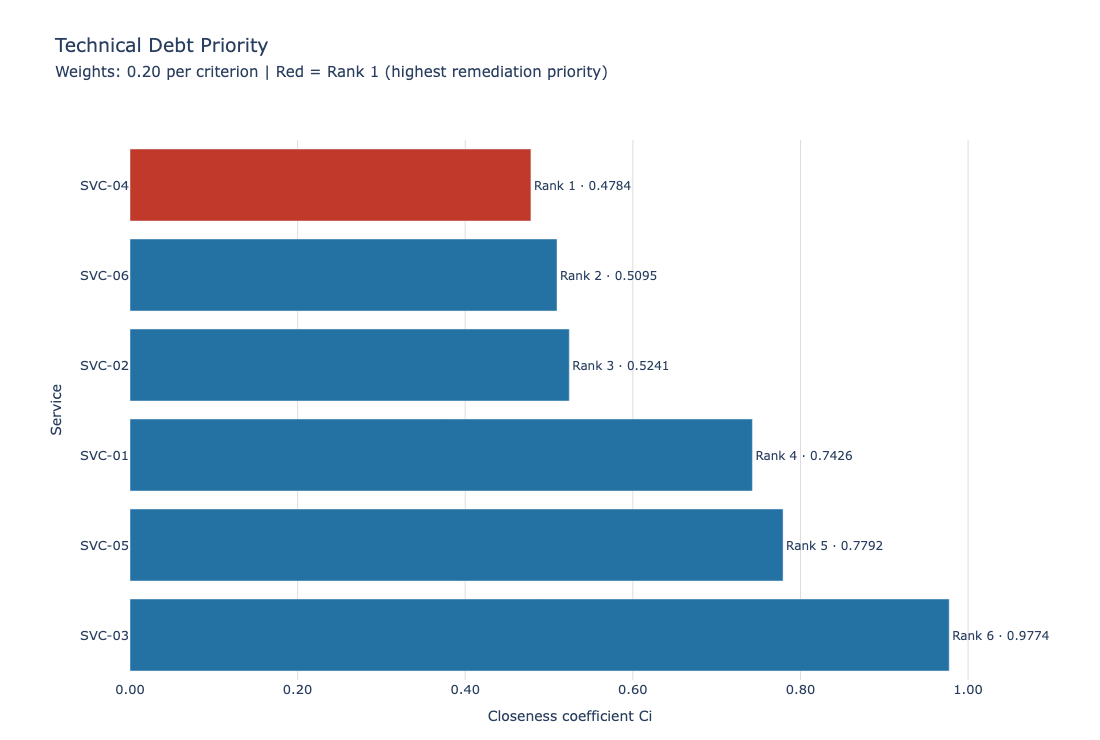
\includegraphics[keepaspectratio]{images/topsis_ranking2025_equal.png}}

}

\caption{\label{fig-topsis-equal-2025}Technical debt priority ranking
for 2025, equal weights.}

\end{figure}%

\begin{figure}[H]

\centering{

\pandocbounded{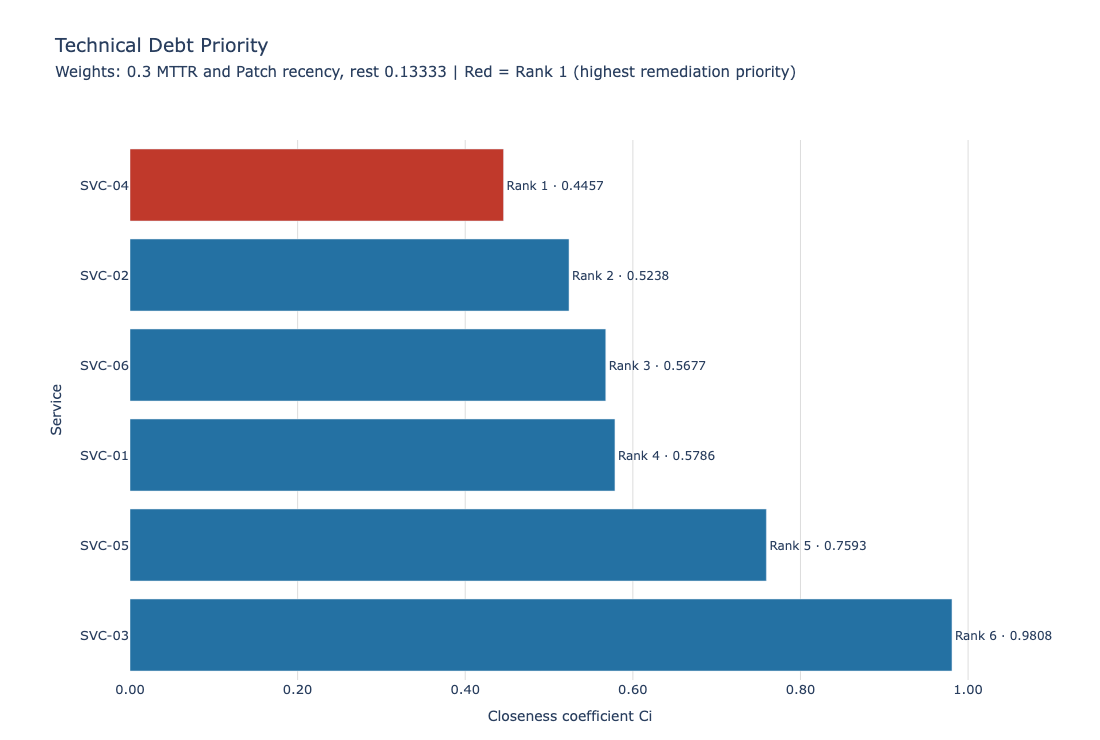
\includegraphics[keepaspectratio]{images/topsis_ranking2025_adjust.png}}

}

\caption{\label{fig-topsis-adjusted-2025}Technical debt priority ranking
for 2025, adjusted weights.}

\end{figure}%

Temporal stability under the adjusted configuration is perfect
(\(\tau = 1.000\), \(p = 0.003\)): the ordering is identical across both
years. Under equal weights it stays strong (\(\tau = 0.867\),
\(p = 0.017\)), with only SVC-01 and SVC-05 trading ranks 4 and 5. That
reflects a real year-on-year shift in their incident, recovery and patch
profiles rather than instability in the model.

The 2024 weight sensitivity result (\(\tau = 0.733\), \(p = 0.056\)) is
the weakest in the set. Two pairs swap rather than the single swap seen
in 2025, because the middle-ranking services have more tightly grouped
scores in 2024, making their order more sensitive to a change in
weights. This is not a structural weakness; it shows that differential
weighting matters more when services carry similar profiles.

\begin{figure}[H]

\centering{

\pandocbounded{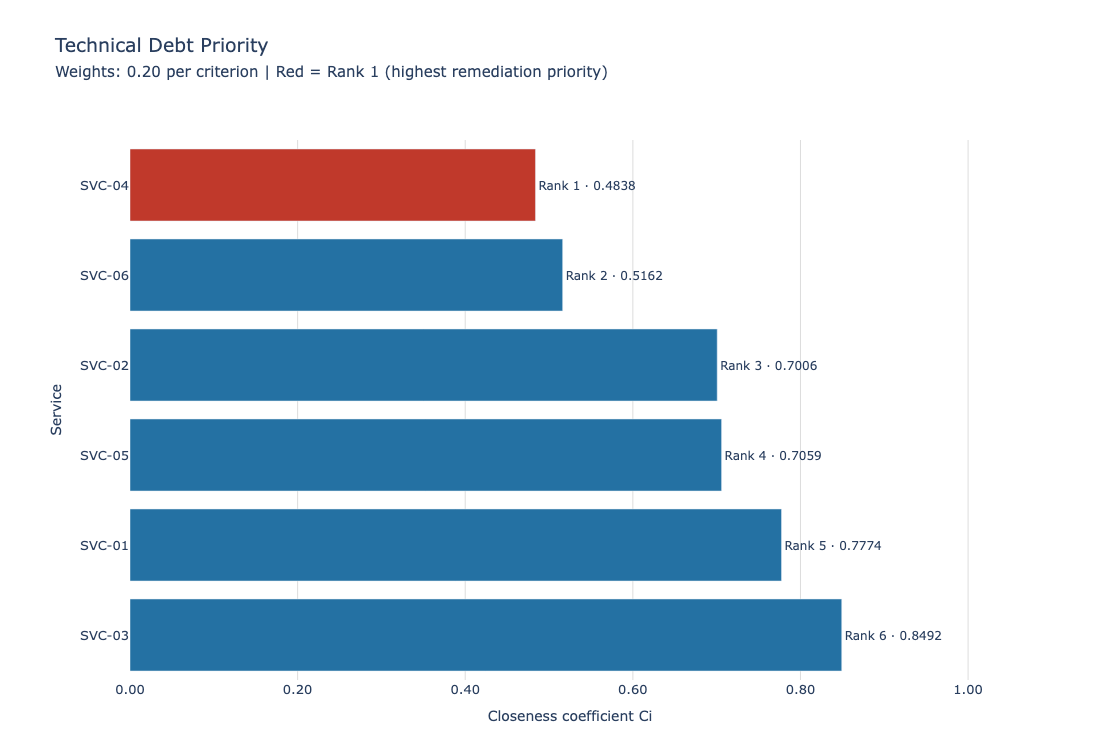
\includegraphics[keepaspectratio]{images/topsis_ranking2024_equal.png}}

}

\caption{\label{fig-topsis-equal-2024}Technical debt priority ranking
for 2024, equal weights.}

\end{figure}%

\begin{figure}[H]

\centering{

\pandocbounded{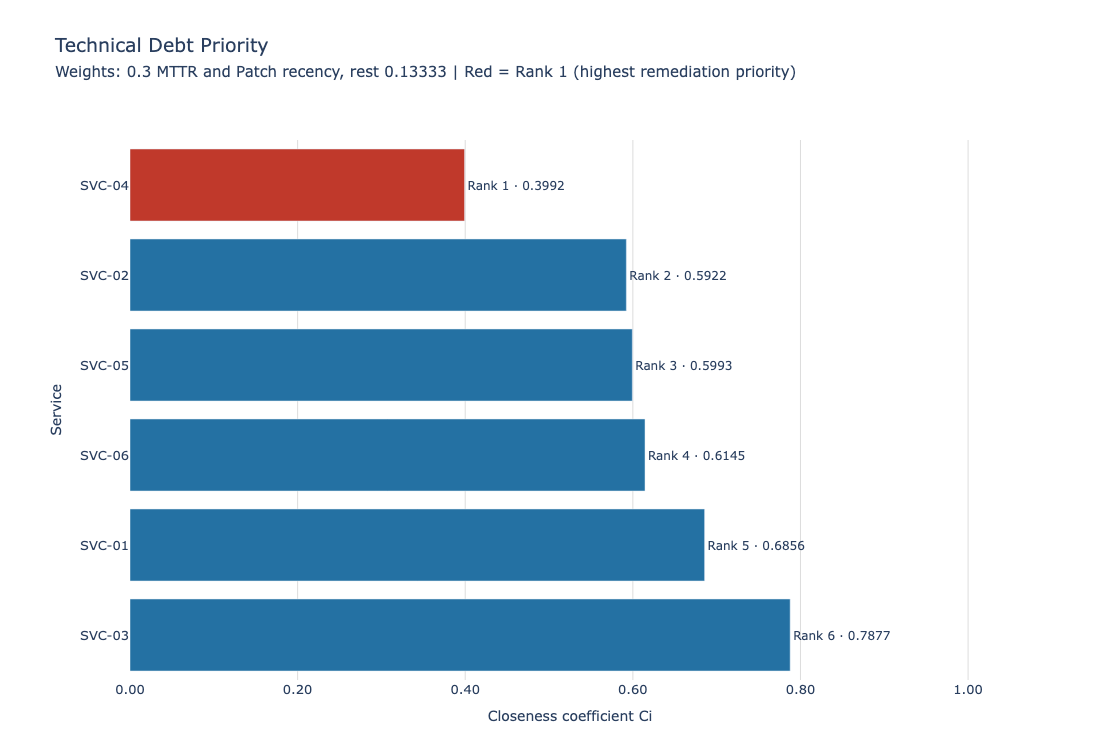
\includegraphics[keepaspectratio]{images/topsis_ranking2024_adjust.png}}

}

\caption{\label{fig-topsis-adjusted-2024}Technical debt priority ranking
for 2024, adjusted weights.}

\end{figure}%

Taken together, these results address RQ3 directly: the rankings are
robust to reasonable variation in criterion weights and consistent
across observation years, with the top and bottom positions stable in
every run.

\section{Convergent Validity Across Methods}\label{sec-convergent}

To test convergent validity, the six services were re-ranked with SAW
and VIKOR and each ordering compared against the TOPSIS result. Because
the dataset contains zero values, SAW used Weitendorf (min-max)
normalisation, which avoids the division by zero that classic cost
normalisation would produce (Thien, Dung and Trung, 2024). VIKOR
followed the standard S, R and Q procedure with \(v = 0.5\).
Table~\ref{tbl-method-agreement} reports agreement across both
configurations and years; Table~\ref{tbl-method-ranks} gives the ranks
each method assigns in the 2025 equal-weight reference case.

Agreement is moderate rather than exact, with \(\tau\) from 0.600 to
0.867, and the pattern behind those figures is consistent. All three
methods place the same three services in the high-priority half and the
same three in the low-priority half, and SVC-03 comes last under every
method, configuration and year. They part company only on the internal
order of the high-priority cluster: TOPSIS ranks SVC-04 first, on its
very high incident volume and CFR, whereas SAW and VIKOR both promote
SVC-06, whose worst-in-portfolio patch recency and high
unsupported-component exposure give it the largest single-criterion
regret. The broad prioritisation is therefore largely independent of
method, even though the single highest-priority service is not. That
matters when the framework informs an individual remediation choice
rather than portfolio-level triage, a limitation revisited in
Section~\ref{sec-evaluationlimitations}.

\begin{longtable}[]{@{}
  >{\raggedright\arraybackslash}p{(\linewidth - 4\tabcolsep) * \real{0.5000}}
  >{\raggedleft\arraybackslash}p{(\linewidth - 4\tabcolsep) * \real{0.2500}}
  >{\raggedleft\arraybackslash}p{(\linewidth - 4\tabcolsep) * \real{0.2500}}@{}}
\caption{Rank agreement (Kendall's \(\tau\)) between TOPSIS and the two
alternative methods.}\label{tbl-method-agreement}\tabularnewline
\toprule\noalign{}
\begin{minipage}[b]{\linewidth}\raggedright
Configuration
\end{minipage} & \begin{minipage}[b]{\linewidth}\raggedleft
TOPSIS vs SAW
\end{minipage} & \begin{minipage}[b]{\linewidth}\raggedleft
TOPSIS vs VIKOR
\end{minipage} \\
\midrule\noalign{}
\endfirsthead
\toprule\noalign{}
\begin{minipage}[b]{\linewidth}\raggedright
Configuration
\end{minipage} & \begin{minipage}[b]{\linewidth}\raggedleft
TOPSIS vs SAW
\end{minipage} & \begin{minipage}[b]{\linewidth}\raggedleft
TOPSIS vs VIKOR
\end{minipage} \\
\midrule\noalign{}
\endhead
\bottomrule\noalign{}
\endlastfoot
2025, equal weights & 0.867 & 0.867 \\
2025, adjusted weights & 0.600 & 0.600 \\
2024, equal weights & 0.733 & 0.867 \\
2024, adjusted weights & 0.733 & 0.600 \\
\end{longtable}

\begin{longtable}[]{@{}
  >{\raggedright\arraybackslash}p{(\linewidth - 6\tabcolsep) * \real{0.4000}}
  >{\raggedleft\arraybackslash}p{(\linewidth - 6\tabcolsep) * \real{0.2000}}
  >{\raggedleft\arraybackslash}p{(\linewidth - 6\tabcolsep) * \real{0.2000}}
  >{\raggedleft\arraybackslash}p{(\linewidth - 6\tabcolsep) * \real{0.2000}}@{}}
\caption{Debt-priority rank by method, 2025 equal
weights.}\label{tbl-method-ranks}\tabularnewline
\toprule\noalign{}
\begin{minipage}[b]{\linewidth}\raggedright
Service
\end{minipage} & \begin{minipage}[b]{\linewidth}\raggedleft
TOPSIS
\end{minipage} & \begin{minipage}[b]{\linewidth}\raggedleft
SAW
\end{minipage} & \begin{minipage}[b]{\linewidth}\raggedleft
VIKOR
\end{minipage} \\
\midrule\noalign{}
\endfirsthead
\toprule\noalign{}
\begin{minipage}[b]{\linewidth}\raggedright
Service
\end{minipage} & \begin{minipage}[b]{\linewidth}\raggedleft
TOPSIS
\end{minipage} & \begin{minipage}[b]{\linewidth}\raggedleft
SAW
\end{minipage} & \begin{minipage}[b]{\linewidth}\raggedleft
VIKOR
\end{minipage} \\
\midrule\noalign{}
\endhead
\bottomrule\noalign{}
\endlastfoot
SVC-04 & 1 & 2 & 2 \\
SVC-06 & 2 & 1 & 1 \\
SVC-02 & 3 & 3 & 3 \\
SVC-01 & 4 & 4 & 4 \\
SVC-05 & 5 & 5 & 5 \\
SVC-03 & 6 & 6 & 6 \\
\end{longtable}

\section{Discriminant Value Against a Single-Criterion
Baseline}\label{sec-discriminant}

Discriminant value was tested against the simplest single-signal
alternative: a ranking by incident frequency alone. The two orderings
diverge, with Kendall's \(\tau\) of 0.600 in 2025 and 0.200 in 2024, and
Table~\ref{tbl-discriminant} sets out the 2025 comparison. The
divergence concentrates in two services. SVC-02 rises against the
incident-only view because its infrastructure-lifecycle debt, carried in
unsupported-component exposure and low patch recency, is invisible to an
incident count, while SVC-05 falls because its high incident volume is
offset by full patch recency and no unsupported components. This is the
value the multi-criteria design adds over a single operational signal,
consistent with Albarak \emph{et al.} (2022), who found that
multi-criteria prioritisation surfaces items single-factor approaches
defer. The wider divergence in 2024 is the same mechanism operating more
strongly: services carrying infrastructure or recovery-time debt, but
only modest incident counts rank far higher under the framework than
under incident volume alone.

\begin{longtable}[]{@{}
  >{\raggedright\arraybackslash}p{(\linewidth - 6\tabcolsep) * \real{0.2800}}
  >{\raggedleft\arraybackslash}p{(\linewidth - 6\tabcolsep) * \real{0.2400}}
  >{\raggedleft\arraybackslash}p{(\linewidth - 6\tabcolsep) * \real{0.2400}}
  >{\raggedleft\arraybackslash}p{(\linewidth - 6\tabcolsep) * \real{0.2400}}@{}}
\caption{TOPSIS rank against an incident-frequency ranking, 2025 equal
weights.}\label{tbl-discriminant}\tabularnewline
\toprule\noalign{}
\begin{minipage}[b]{\linewidth}\raggedright
Service
\end{minipage} & \begin{minipage}[b]{\linewidth}\raggedleft
TOPSIS rank
\end{minipage} & \begin{minipage}[b]{\linewidth}\raggedleft
Incident-only rank
\end{minipage} & \begin{minipage}[b]{\linewidth}\raggedleft
Shift
\end{minipage} \\
\midrule\noalign{}
\endfirsthead
\toprule\noalign{}
\begin{minipage}[b]{\linewidth}\raggedright
Service
\end{minipage} & \begin{minipage}[b]{\linewidth}\raggedleft
TOPSIS rank
\end{minipage} & \begin{minipage}[b]{\linewidth}\raggedleft
Incident-only rank
\end{minipage} & \begin{minipage}[b]{\linewidth}\raggedleft
Shift
\end{minipage} \\
\midrule\noalign{}
\endhead
\bottomrule\noalign{}
\endlastfoot
SVC-04 & 1 & 1 & 0 \\
SVC-06 & 2 & 2 & 0 \\
SVC-02 & 3 & 5 & +2 \\
SVC-01 & 4 & 4 & 0 \\
SVC-05 & 5 & 3 & -2 \\
SVC-03 & 6 & 6 & 0 \\
\end{longtable}

\section{Rank Reversal}\label{sec-rankreversal}

Structural rigour was examined with a rank-reversal test: each service
was removed in turn and the remainder re-ranked.
Table~\ref{tbl-rankreversal} reports the 2025 equal-weight results. The
order holds in three of the six removals. In the other three, a single
adjacent pair changes places: removing SVC-02 swaps the two
highest-priority services, SVC-04 and SVC-06, while removing either
SVC-04 or SVC-06 swaps the middle pair, SVC-01 and SVC-05. Each affected
pair sits within a narrow closeness-coefficient margin, and no service
crosses between the high-priority and low-priority halves under any
removal; the lowest-priority service never moves. Rank reversal is
therefore present but confined to fine ordering within already adjacent
clusters, the familiar limitation of distance-based aggregation
identified by García-Cascales and Lamata (2012). Where a fixed reference
frame is required, the normalisation proposed by Yang (2020) removes the
effect.

\begin{longtable}[]{@{}
  >{\raggedright\arraybackslash}p{(\linewidth - 2\tabcolsep) * \real{0.3500}}
  >{\raggedright\arraybackslash}p{(\linewidth - 2\tabcolsep) * \real{0.6500}}@{}}
\caption{Effect of removing each service on the order of the remaining
five, 2025 equal weights.}\label{tbl-rankreversal}\tabularnewline
\toprule\noalign{}
\begin{minipage}[b]{\linewidth}\raggedright
Service removed
\end{minipage} & \begin{minipage}[b]{\linewidth}\raggedright
Outcome
\end{minipage} \\
\midrule\noalign{}
\endfirsthead
\toprule\noalign{}
\begin{minipage}[b]{\linewidth}\raggedright
Service removed
\end{minipage} & \begin{minipage}[b]{\linewidth}\raggedright
Outcome
\end{minipage} \\
\midrule\noalign{}
\endhead
\bottomrule\noalign{}
\endlastfoot
SVC-01 & Order preserved \\
SVC-02 & SVC-04 and SVC-06 exchange ranks 1 and 2 \\
SVC-03 & Order preserved \\
SVC-04 & SVC-01 and SVC-05 exchange ranks \\
SVC-05 & Order preserved \\
SVC-06 & SVC-01 and SVC-05 exchange ranks \\
\end{longtable}

\section{Practical Validity}\label{sec-practicalvalidity}

SVC-04 holds rank 1 in all four calculations, the highest technical debt
priority in the portfolio. Its 2025 profile pairs the highest incident
frequency, 574 per year, with an MTTR of 41.91 hours and a CFR of 3.38,
yet carries no unsupported components and full patch recency. The high
incident volume and change failure rate point to debt that is
operational rather than infrastructural, consistent with the
architectural debt symptoms described in the literature (Ramasubbu and
Kemerer, 2021; de Toledo \emph{et al.}, 2021).

At the other end, SVC-03 has the lowest debt priority in every run: the
fewest incidents, a low MTTR, a low CFR, full patch recency and no
unsupported components. This profile anchors the negative ideal solution
and offers a concrete reference for a well-maintained service.

The most revealing service is SVC-02. It ranks third under equal weights
and rises to second under adjusted weights, driven by an unsupported
component months value of 1,221, by far the largest in the portfolio,
together with the lowest patch recency score. This is exactly the signal
the framework is built to surface: a service that looks operationally
stable in isolation but carries structural debt only multi-criteria
analysis brings into view, consistent with the infrastructure lifecycle
debt category described by Haki \emph{et al.} (2023).

These results address RQ2. A strict causal claim cannot be drawn from
cross-sectional data alone, but the rankings match the operational debt
profiles the literature would predict for each position (Ramasubbu and
Kemerer, 2021; Nord, Ozkaya and Woody, 2021; Haki \emph{et al.}, 2023).
The framework yields an ordinal priority signal that can be read against
the debt dimensions mapped in Table~\ref{tbl-indicators-lit}.

\section{Limitations of the Evaluation}\label{sec-evaluationlimitations}

The most fundamental limitation is that every strand of the evaluation
draws on the same dataset and indicator set used to build the framework.
The triangulation and baseline comparisons establish convergent and
discriminant validity, but not criterion validity against an independent
measure of technical debt, because no such measure exists for the
non-code debt in scope. External validation is therefore the main avenue
for future work.

The small portfolio of six services limits the power of the Kendall's
tau tests. A concordance of \(\tau = 0.733\) cannot reach significance
at the conventional threshold when only 720 permutations are possible,
even though the agreement it represents is substantively meaningful. A
larger service set would ease this constraint.

The cross-sectional design captures only a snapshot. A service that has
recently completed significant remediation may look worse than its
current state warrants, while one whose debt is still growing may not
yet show the full consequences within a single annual window.
Longitudinal evaluation is flagged as a priority for future work in
Chapter~\ref{sec-chapter6}.

Finally, the data quality limitations set out in
Section~\ref{sec-datalimitations} apply here too. Inconsistent incident
recording, partial issue capture split across the organisation's ITSM
platform and its issue tracker, and the dependence of CFR on
documentation discipline all add noise to the input. The stability
results offset this in part, but middle-position rankings still warrant
careful reading.

\bookmarksetup{startatroot}

\chapter{Conclusion}\label{sec-chapter6}

\section{Research Summary}\label{research-summary}

\section{Findings Against Research
Questions}\label{findings-against-research-questions}

\section{Contribution to Knowledge}\label{contribution-to-knowledge}

\section{Practical Contribution}\label{practical-contribution}

\section{Limitations and Future Work}\label{limitations-and-future-work}

\section{Reflective Note}\label{reflective-note}

\bookmarksetup{startatroot}

\chapter*{References}\label{references}
\addcontentsline{toc}{chapter}{References}

\markboth{References}{References}

\phantomsection\label{refs}
\begin{CSLReferences}{0}{1}
\bibitem[\citeproctext]{ref-ahmadTechnicalDebtNot2026}
Ahmad, M.O., Mandić, V., Taušan, N., Katin, A. and Herath, P. (2026)
\textquotesingle Technical debt is not just technical: {An} industrial
case study in large agile software development\textquotesingle,
\emph{Journal of Systems and Software}, 234, p. 112719. Available at:
\url{https://doi.org/10.1016/j.jss.2025.112719}.

\bibitem[\citeproctext]{ref-albarakManagingTechnicalDebt2022}
Albarak, M., Bahsoon, R., Ozkaya, I. and Nord, R.L. (2022)
\textquotesingle Managing {Technical Debt} in {Database
Normalization}\textquotesingle, \emph{IEEE Transactions on Software
Engineering}, 48(3), pp. 755--772. Available at:
\url{https://doi.org/10.1109/TSE.2020.3001339}.

\bibitem[\citeproctext]{ref-albuquerqueManagingTechnicalDebt2023}
Albuquerque, D., Guimarães, E., Tonin, G., Rodríguezs, P., Perkusich,
M., Almeida, H., Perkusich, A. and Chagas, F. (2023)
\textquotesingle Managing {Technical Debt Using Intelligent Techniques}
- {A Systematic Mapping Study}\textquotesingle, \emph{IEEE Transactions
on Software Engineering}, 49(4), pp. 2202--2220. Available at:
\url{https://doi.org/10.1109/TSE.2022.3214764}.

\bibitem[\citeproctext]{ref-alfayezHowSonarQubeidentifiedTechnical2023}
Alfayez, R., Winn, R., Alwehaibi, W., Venson, E. and Boehm, B. (2023)
\textquotesingle How {SonarQube-identified} technical debt is
prioritized: {An} exploratory case study\textquotesingle,
\emph{Information and Software Technology}, 156, p. 107147. Available
at: \url{https://doi.org/10.1016/j.infsof.2023.107147}.

\bibitem[\citeproctext]{ref-amanatidisEvaluatingAgreementTechnical2020}
Amanatidis, T., Mittas, N., Moschou, A., Chatzigeorgiou, A.,
Ampatzoglou, A. and Angelis, L. (2020) \textquotesingle Evaluating the
agreement among technical debt measurement tools: Building an empirical
benchmark of technical debt liabilities\textquotesingle, \emph{Empirical
Software Engineering}, 25(5), pp. 4161--4204. Available at:
\url{https://doi.org/10.1007/s10664-020-09869-w}.

\bibitem[\citeproctext]{ref-ampatzoglouSDK4EDPlatformTechnical2022}
Ampatzoglou, A., Chatzigeorgiou, A., Arvanitou, E.M. and Bibi, S. (2022)
\textquotesingle{}{SDK4ED}: {A} platform for technical debt
management\textquotesingle, \emph{Software: Practice and Experience},
52(8), pp. 1879--1902. Available at:
\url{https://doi.org/10.1002/spe.3093}.

\bibitem[\citeproctext]{ref-avgeriouTechnicalDebtManagement2023}
Avgeriou, P., Ozkaya, I., Chatzigeorgiou, A., Ciolkowski, M., Ernst,
N.A., Koontz, R.J., Poort, E. and Shull, F. (2023)
\textquotesingle Technical {Debt Management}: {The Road Ahead} for
{Successful Software Delivery}\textquotesingle, \emph{2023 {IEEE}/{ACM
International Conference} on {Software Engineering}: {Future} of
{Software Engineering} ({ICSE-FoSE})}. \emph{2023 {IEEE}/{ACM
International Conference} on {Software Engineering}: {Future} of
{Software Engineering} ({ICSE-FoSE})}, Melbourne, Australia: IEEE, pp.
15--30. Available at:
\url{https://doi.org/10.1109/ICSE-FoSE59343.2023.00007}.

\bibitem[\citeproctext]{ref-bankerTechnicalDebtFirm2020}
Banker, R., Liang, Y. and Ramasubbu, N. (2020)
\textquotesingle Technical {Debt} and {Firm
Performance}\textquotesingle, \emph{Management Science}, 67(5), pp.
3174--3194. Available at: \url{https://doi.org/10.1287/mnsc.2019.3542}.

\bibitem[\citeproctext]{ref-bediUnderstandingFactorsAffecting2022}
Bedi, J. and Kaur, K. (2022) \textquotesingle Understanding factors
affecting technical debt\textquotesingle, \emph{International Journal of
Information Technology}, 14(2), pp. 1051--1060. Available at:
\url{https://doi.org/10.1007/s41870-020-00487-9}.

\bibitem[\citeproctext]{ref-beskerTechnicalDebtEmpirical2020}
Besker, T. (2020) \emph{Technical {Debt}: {An} empirical investigation
of its harmfulness and on management strategies in industry}. Chalmers
University of Technology. Available at:
\url{https://research.chalmers.se/publication/518318/file/518318_Fulltext.pdf}.

\bibitem[\citeproctext]{ref-biazottoTechnicalDebtManagement2024}
Biazotto, J.P., Feitosa, D., Avgeriou, P. and Nakagawa, E.Y. (2024)
\textquotesingle Technical debt management automation: {State} of the
art and future perspectives\textquotesingle, \emph{Information and
Software Technology}, 167, p. 107375. Available at:
\url{https://doi.org/10.1016/j.infsof.2023.107375}.

\bibitem[\citeproctext]{ref-chenRolesChallengesMerits2023}
Chén, O.Y., Bodelet, J.S., Saraiva, R.G., Phan, H., Di, J., Nagels, G.,
Schwantje, T., Cao, H., Gou, J., Reinen, J.M., Xiong, B., Zhi, B., Wang,
X. and Vos, M. de (2023) \textquotesingle The roles, challenges, and
merits of the p value\textquotesingle, \emph{Patterns}, 4(12), p.
100878. Available at:
\url{https://doi.org/10.1016/j.patter.2023.100878}.

\bibitem[\citeproctext]{ref-ciardielloComparisonTOPSISSAW2023}
Ciardiello, F. and Genovese, A. (2023) \textquotesingle A comparison
between {TOPSIS} and {SAW} methods\textquotesingle, \emph{Annals of
Operations Research}, 325(2), pp. 967--994. Available at:
\url{https://doi.org/10.1007/s10479-023-05339-w}.

\bibitem[\citeproctext]{ref-CodeConductBCS2022}
\emph{Code of {Conduct} for {BCS Members}} (2022). Swindon, UK: BCS, The
Chartered Institute for IT, pp. 1--5. Available at:
\url{https://www.bcs.org/media/2211/bcs-code-of-conduct.pdf} (Accessed:
April 15, 2026).

\bibitem[\citeproctext]{ref-cunninghamWyCashPortfolioManagement1992}
Cunningham, W. (1992) \textquotesingle The {WyCash} portfolio management
system\textquotesingle, \emph{ACM SIGPLAN OOPS Messenger}, 4(2), pp.
29--30. Available at: \url{https://doi.org/10.1145/157710.157715}.

\bibitem[\citeproctext]{ref-FederalActData2023}
\emph{Federal {Act} on {Data Protection}} (2023). Available at:
\url{https://www.fedlex.admin.ch/eli/cc/2022/491/en} (Accessed: April
15, 2026).

\bibitem[\citeproctext]{ref-finmaCircular202312024}
\emph{{FINMA Circular} 2023/1 - {Operational} risks and resilience --
banks} (2024). Available at:
\url{https://www.finma.ch/en/~/media/finma/dokumente/dokumentencenter/myfinma/rundschreiben/finma-rs-2023-01-20221207.pdf}
(Accessed: March 29, 2026).

\bibitem[\citeproctext]{ref-forsgrenAccelerate2018}
Forsgren, N., Humble, J. and Kim, G. (2018) \emph{Accelerate: {The
Science} of {Lean Software} and {DevOps}: {Building} and {Scaling High
Performing Technology Organizations}}. Portland, OR: IT Revolution
Press.

\bibitem[\citeproctext]{ref-fowlerTechnicalDebtQuadrant2009}
Fowler, M. (2009) \emph{Technical {Debt Quadrant}}. Technical Debt
Quadrant. Available at:
\url{https://martinfowler.com/bliki/TechnicalDebtQuadrant.html}
(Accessed: March 29, 2026).

\bibitem[\citeproctext]{ref-garcia-cascalesRankReversalTOPSIS2012}
García-Cascales, M.S. and Lamata, M.T. (2012) \textquotesingle On rank
reversal and {TOPSIS} method\textquotesingle, \emph{Mathematical and
Computer Modelling}, 56(5), pp. 123--132. Available at:
\url{https://doi.org/10.1016/j.mcm.2011.12.022}.

\bibitem[\citeproctext]{ref-grecoMethodologicalFrameworkComposite2019}
Greco, S., Ishizaka, A., Tasiou, M. and Torrisi, G. (2019)
\textquotesingle On the {Methodological Framework} of {Composite
Indices}: {A Review} of the {Issues} of {Weighting}, {Aggregation}, and
{Robustness}\textquotesingle, \emph{Social Indicators Research}, 141(1),
pp. 61--94. Available at:
\url{https://doi.org/10.1007/s11205-017-1832-9}.

\bibitem[\citeproctext]{ref-hakiDigitalNudgingTechnical2023}
Haki, K., Rieder, A., Buchmann, L. and Schneider, A.W. (2023)
\textquotesingle Digital nudging for technical debt management at
{Credit Suisse}\textquotesingle, \emph{European Journal of Information
Systems}, 32(1), pp. 64--80. Available at:
\url{https://doi.org/10.1080/0960085X.2022.2088413}.

\bibitem[\citeproctext]{ref-hanssenIdentifyingScalabilityDebt2019}
Hanssen, G.K., Brataas, G. and Martini, A. (2019)
\textquotesingle Identifying {Scalability Debt} in {Open
Systems}\textquotesingle, \emph{2019 {IEEE}/{ACM International
Conference} on {Technical Debt} ({TechDebt})}. \emph{2019 {IEEE}/{ACM
International Conference} on {Technical Debt} ({TechDebt})}, pp. 48--52.
Available at: \url{https://doi.org/10.1109/TechDebt.2019.00014}.

\bibitem[\citeproctext]{ref-hevnerDesignScienceInformation2004}
Hevner, A.R., March, S.T., Park, J. and Ram, S. (2004)
\textquotesingle Design {Science} in {Information Systems
Research}\textquotesingle, \emph{MIS Quarterly}, 28(1), pp. 75--105.
Available at: \url{https://doi.org/10.2307/25148625}.

\bibitem[\citeproctext]{ref-hwangMultipleAttributeDecision1981}
Hwang, C.-L. and Yoon, K. (1981) \emph{Multiple {Attribute Decision
Making}}. Edited by M. Beckmann and H.P. Künzi. Berlin, Heidelberg:
Springer (Lecture {Notes} in {Economics} and {Mathematical Systems}).
Available at: \url{https://doi.org/10.1007/978-3-642-48318-9}.

\bibitem[\citeproctext]{ref-ishakAnalysisFuzzyAHPTOPSIS2020}
Ishak, A. and Wanli (2020) \textquotesingle Analysis of {Fuzzy
AHP-TOPSIS Methods} in {Multi Criteria Decision Making}: {Literature
Review}\textquotesingle, \emph{IOP Conference Series: Materials Science
and Engineering}, 1003(1), p. 012147. Available at:
\url{https://doi.org/10.1088/1757-899X/1003/1/012147}.

\bibitem[\citeproctext]{ref-kellyThreePrinciplesPragmatism2020}
Kelly, L.M. and Cordeiro, M. (2020) \textquotesingle Three principles of
pragmatism for research on organizational processes\textquotesingle,
\emph{Methodological Innovations}, 13(2), p. 2059799120937242. Available
at: \url{https://doi.org/10.1177/2059799120937242}.

\bibitem[\citeproctext]{ref-khanIntegratedMethodologyRanking2022}
Khan, S. and Purohit, L. (2022) \textquotesingle An {Integrated
Methodology} of {Ranking Based} on {PROMETHEE-CRITIC} and {TOPSIS-CRITIC
In Web Service Domain}\textquotesingle, \emph{2022 {IEEE} 11th
{International Conference} on {Communication Systems} and {Network
Technologies} ({CSNT})}. \emph{2022 {IEEE} 11th {International
Conference} on {Communication Systems} and {Network Technologies}
({CSNT})}, pp. 335--340. Available at:
\url{https://doi.org/10.1109/CSNT54456.2022.9787620}.

\bibitem[\citeproctext]{ref-kleinwaksTechnicalDebtSystems2023}
Kleinwaks, H., Batchelor, A. and Bradley, T.H. (2023)
\textquotesingle Technical debt in systems engineering---{A} systematic
literature review\textquotesingle, \emph{Systems Engineering}, 26(5),
pp. 675--687. Available at: \url{https://doi.org/10.1002/sys.21681}.

\bibitem[\citeproctext]{ref-kruchtenTechnicalDebtMetaphor2012}
Kruchten, P., Nord, R.L. and Ozkaya, I. (2012)
\textquotesingle Technical {Debt}: {From Metaphor} to {Theory} and
{Practice}\textquotesingle, \emph{IEEE Software}, 29(6), pp. 18--21.
Available at: \url{https://doi.org/10.1109/MS.2012.167}.

\bibitem[\citeproctext]{ref-kulaReleasingFastSlow2019}
Kula, E., Rastogi, A., Huijgens, H., Deursen, A. van and Gousios, G.
(2019) \textquotesingle Releasing fast and slow: An exploratory case
study at {ING}\textquotesingle, \emph{Proceedings of the 2019 27th {ACM
Joint Meeting} on {European Software Engineering Conference} and
{Symposium} on the {Foundations} of {Software Engineering}}. New York,
NY, USA: Association for Computing Machinery ({ESEC}/{FSE} 2019), pp.
785--795. Available at: \url{https://doi.org/10.1145/3338906.3338978}.

\bibitem[\citeproctext]{ref-lenarduzziSystematicLiteratureReview2021}
Lenarduzzi, V., Besker, T., Taibi, D., Martini, A. and Arcelli Fontana,
F. (2021) \textquotesingle A systematic literature review on {Technical
Debt} prioritization: {Strategies}, processes, factors, and
tools\textquotesingle, \emph{Journal of Systems and Software}, 171, p.
110827. Available at: \url{https://doi.org/10.1016/j.jss.2020.110827}.

\bibitem[\citeproctext]{ref-markkanenPatchManagementPlanning2023}
Markkanen, V. and Frantti, T. (2023) \textquotesingle Patch management
planning - towards one-to-one policy\textquotesingle, \emph{2023 10th
{International Conference} on {Dependable Systems} and {Their
Applications} ({DSA})}. \emph{2023 10th {International Conference} on
{Dependable Systems} and {Their Applications} ({DSA})}, pp. 60--69.
Available at: \url{https://doi.org/10.1109/DSA59317.2023.00018}.

\bibitem[\citeproctext]{ref-mcconnellManagingTechnicalDebt2008}
McConnell, S. (2008) \textquotesingle Managing {Technical
Debt}\textquotesingle. Construx Software. Available at:
\url{https://www.construx.com/wp-content/uploads/2019/02/CxWhitePaper_TechnicalDebt.pdf}
(Accessed: March 21, 2026).

\bibitem[\citeproctext]{ref-nielsenITPortfolioManagement2022}
Nielsen, M.E. and Skaarup, S. (2022) \textquotesingle{}{IT Portfolio}
management as a framework for managing {Technical Debt}: {Theoretical}
framework applied on a case study\textquotesingle, \emph{14th
{International Conference} on {Theory} and {Practice} of {Electronic
Governance}}. \emph{{ICEGOV} 2021: 14th {International Conference} on
{Theory} and {Practice} of {Electronic Governance}}, New York, NY, USA:
Association for Computing Machinery, pp. 89--96. Available at:
\url{https://doi.org/10.1145/3494193.3494296}.

\bibitem[\citeproctext]{ref-nordExamplesTechnicalDebts2021}
Nord, R.L., Ozkaya, I. and Woody, C. (2021) \emph{Examples of {Technical
Debt}'s {Cybersecurity Impact}}. Pittsburgh, PA, USA: Carnegie Mellon
University, pp. 1--21. Available at:
\url{https://apps.dtic.mil/sti/trecms/pdf/AD1144728.pdf} (Accessed:
April 27, 2026).

\bibitem[\citeproctext]{ref-nursePatchNotPatch2025}
Nurse, J.R.C. (2025) \textquotesingle To {Patch} or~{Not} to~{Patch}:
{Motivations}, {Challenges}, and~{Implications}
for~{Cybersecurity}\textquotesingle, in A. Moallem (ed.) \emph{{HCI} for
{Cybersecurity}, {Privacy} and {Trust}}. Cham: Springer Nature
Switzerland, pp. 265--281. Available at:
\url{https://doi.org/10.1007/978-3-031-92833-8_16}.

\bibitem[\citeproctext]{ref-pandeyReviewTOPSISMethod2023}
Pandey, V., Komal and Dincer, H. (2023) \textquotesingle A review on
{TOPSIS} method and its extensions for different applications with
recent development\textquotesingle, \emph{Soft Computing}, 27(23), pp.
18011--18039. Available at:
\url{https://doi.org/10.1007/s00500-023-09011-0}.

\bibitem[\citeproctext]{ref-paudelExploringRelationshipTechnical2025}
Paudel, B., Gonzalez-Huerta, J., Zabardast, E. and Klotins, E. (2025)
\textquotesingle Exploring the {Relationship Between Technical Debt} and
{Lead Time}: {An Industrial Case Study}\textquotesingle, \emph{2025
{IEEE International Conference} on {Software Analysis}, {Evolution} and
{Reengineering} ({SANER})}. \emph{2025 {IEEE International Conference}
on {Software Analysis}, {Evolution} and {Reengineering} ({SANER})}, pp.
693--703. Available at:
\url{https://doi.org/10.1109/SANER64311.2025.00071}.

\bibitem[\citeproctext]{ref-pinaTechnicalDebtPrioritization2022}
Pina, D., Seaman, C. and Goldman, A. (2022) \textquotesingle Technical
{Debt Prioritization}: {A Developer}'s {Perspective}\textquotesingle,
\emph{2022 {IEEE}/{ACM International Conference} on {Technical Debt}
({TechDebt})}. \emph{2022 {IEEE}/{ACM International Conference} on
{Technical Debt} ({TechDebt})}, pp. 46--55. Available at:
\url{https://doi.org/10.1145/3524843.3528096}.

\bibitem[\citeproctext]{ref-ramasubbuControllingTechnicalDebt2021}
Ramasubbu, N. and Kemerer, C.F. (2021) \textquotesingle Controlling
{Technical Debt Remediation} in {Outsourced Enterprise Systems
Maintenance}: {An Empirical Analysis}\textquotesingle, \emph{Journal of
Management Information Systems}, 38(1), pp. 4--28. Available at:
\url{https://doi.org/10.1080/07421222.2021.1870377}.

\bibitem[\citeproctext]{ref-ramasubbuManagingTechnicalDebt2015}
Ramasubbu, N., Kemerer, C.F. and Woodard, C.J. (2015)
\textquotesingle Managing {Technical Debt}: {Insights} from {Recent
Empirical Evidence}\textquotesingle, \emph{IEEE Software}, 32(2), pp.
22--25. Available at: \url{https://doi.org/10.1109/MS.2015.45}.

\bibitem[\citeproctext]{ref-rinta-kahilaGettingTrappedTechnical2023}
Rinta-Kahila, T., Penttinen, E., Aalto University, Lyytinen, K. and Case
Western Reserve University (2023) \textquotesingle Getting {Trapped} in
{Technical Debt}: {Sociotechnical Analysis} of a {Legacy System}'s
{Replacement}\textquotesingle, \emph{MIS Quarterly}, 47(1), pp. 1--32.
Available at: \url{https://doi.org/10.25300/MISQ/2022/16711}.

\bibitem[\citeproctext]{ref-rollandExploringTensionsManagement2021}
Rolland, K.-H. and Lyytinen, K. (2021) \textquotesingle Exploring the
{Tensions Between Management} of {Architectural Debt} and {Digital
Innovation}: {The Case} of a {Financial Organization}\textquotesingle,
\emph{Proceedings of the 54th {Hawaii International Conference} on
{System Sciences}}. \emph{54th {Hawaii International Conference} on
{System Sciences}}, Hawaii International Conference on System Sciences,
pp. 6722--6732. Available at:
\url{https://doi.org/10.24251/HICSS.2021.807}.

\bibitem[\citeproctext]{ref-shekhovtsovHowStronglyRank2021}
Shekhovtsov, A. (2021) \textquotesingle How strongly do rank similarity
coefficients differ used in decision making problems?\textquotesingle,
\emph{Procedia Computer Science}, 192, pp. 4570--4577. Available at:
\url{https://doi.org/10.1016/j.procs.2021.09.235}.

\bibitem[\citeproctext]{ref-shekhovtsovComparativeCaseStudy2020}
Shekhovtsov, A. and Sałabun, W. (2020) \textquotesingle A comparative
case study of the {VIKOR} and {TOPSIS} rankings
similarity\textquotesingle, \emph{Procedia Computer Science}, 176, pp.
3730--3740. Available at:
\url{https://doi.org/10.1016/j.procs.2020.09.014}.

\bibitem[\citeproctext]{ref-stochelBusinessdrivenTechnicalDebt2023}
Stochel, M.G., Borek, T., Wawrowski, M.R. and Chołda, P. (2023)
\textquotesingle Business-driven technical debt management using
{Continuous Debt Valuation Approach} ({CoDVA})\textquotesingle,
\emph{Information and Software Technology}, 164, p. 107333. Available
at: \url{https://doi.org/10.1016/j.infsof.2023.107333}.

\bibitem[\citeproctext]{ref-thienOvercomingLimitationsRAPS2024}
Thien, N.V., Dung, H.T. and Trung, D.D. (2024)
\textquotesingle Overcoming the {Limitations} of the {RAPS Method} by
identifying {Alternative Data Normalization Methods}\textquotesingle,
\emph{Engineering, Technology \& Applied Science Research}, 14(4), pp.
15745--15750. Available at: \url{https://doi.org/10.48084/etasr.7909}.

\bibitem[\citeproctext]{ref-tizioSoftwareUpdatesStrategies2023}
Tizio, G.D., Armellini, M. and Massacci, F. (2023)
\textquotesingle Software {Updates Strategies}: {A Quantitative
Evaluation Against Advanced Persistent Threats}\textquotesingle,
\emph{IEEE Transactions on Software Engineering}, 49(3), pp. 1359--1373.
Available at: \url{https://doi.org/10.1109/TSE.2022.3176674}.

\bibitem[\citeproctext]{ref-detoledoReducingIncidentsMicroservices2021}
de Toledo, S.S., Martini, A., Sjøberg, D.I.K., Przybyszewska, A. and
Frandsen, J.S. (2021) \textquotesingle Reducing {Incidents} in
{Microservices} by {Repaying Architectural Technical
Debt}\textquotesingle, \emph{2021 47th {Euromicro Conference} on
{Software Engineering} and {Advanced Applications} ({SEAA})}. \emph{2021
47th {Euromicro Conference} on {Software Engineering} and {Advanced
Applications} ({SEAA})}, pp. 196--205. Available at:
\url{https://doi.org/10.1109/SEAA53835.2021.00033}.

\bibitem[\citeproctext]{ref-tornhillCodeRedBusiness2022}
Tornhill, A. and Borg, M. (2022) \textquotesingle Code {Red}: {The
Business Impact} of {Code Quality} - {A Quantitative Study} of 39
{Proprietary Production Codebases}\textquotesingle, \emph{2022
{IEEE}/{ACM International Conference} on {Technical Debt} ({TechDebt})}.
\emph{2022 {IEEE}/{ACM International Conference} on {Technical Debt}
({TechDebt})}, pp. 11--20. Available at:
\url{https://doi.org/10.1145/3524843.3528091}.

\bibitem[\citeproctext]{ref-turnbullUseCaseStudy2021}
Turnbull, D., Chugh, R. and Luck, J. (2021) \textquotesingle The {Use}
of {Case Study Design} in {Learning Management System Research}: {A
Label} of {Convenience}?\textquotesingle, \emph{International Journal of
Qualitative Methods}, 20, pp. 1--11. Available at:
\url{https://doi.org/10.1177/16094069211004148}.

\bibitem[\citeproctext]{ref-vidoniInfiniteTechnicalDebt2022}
Vidoni, M., Codabux, Z. and Fard, F.H. (2022) \textquotesingle Infinite
technical debt\textquotesingle, \emph{Journal of Systems and Software},
190, p. 111336. Available at:
\url{https://doi.org/10.1016/j.jss.2022.111336}.

\bibitem[\citeproctext]{ref-vombrockeIntroductionDesignScience2020}
Vom Brocke, J., Hevner, A. and Maedche, A. (2020)
\textquotesingle Introduction to {Design Science
Research}\textquotesingle, in J. Vom Brocke, A. Hevner, and A. Maedche
(eds.) \emph{Design {Science Research}. {Cases}}. Cham: Springer
International Publishing, pp. 1--13. Available at:
\url{https://doi.org/10.1007/978-3-030-46781-4_1}.

\bibitem[\citeproctext]{ref-wieseITManagersPerspective2023}
Wiese, M. and Borowa, K. (2023) \textquotesingle{}{IT} managers'
perspective on {Technical Debt Management}\textquotesingle,
\emph{Journal of Systems and Software}, 202, p. 111700. Available at:
\url{https://doi.org/10.1016/j.jss.2023.111700}.

\bibitem[\citeproctext]{ref-yangIngeniousSolutionRank2020}
Yang, W. (2020) \textquotesingle Ingenious {Solution} for the {Rank
Reversal Problem} of {TOPSIS Method}\textquotesingle, \emph{Mathematical
Problems in Engineering}, 2020(1), p. 9676518. Available at:
\url{https://doi.org/10.1155/2020/9676518}.

\bibitem[\citeproctext]{ref-yangTaxonomyTechnicalDebt2019}
Yang, Y., Michel, R., Wade, J., Verma, D., Törngren, M. and Alelyani, T.
(2019) \textquotesingle Towards a taxonomy of technical debt for
{COTS-intensive} cyber physical systems\textquotesingle, \emph{Procedia
Computer Science}, 153, pp. 108--117. Available at:
\url{https://doi.org/10.1016/j.procs.2019.05.061}.

\bibitem[\citeproctext]{ref-zanakisMultiattributeDecisionMaking1998}
Zanakis, S.H., Solomon, A., Wishart, N. and Dublish, S. (1998)
\textquotesingle Multi-attribute decision making: {A} simulation
comparison of select methods\textquotesingle, \emph{European Journal of
Operational Research}, 107(3), pp. 507--529. Available at:
\url{https://doi.org/10.1016/S0377-2217(97)00147-1}.

\bibitem[\citeproctext]{ref-zytoonDecisionSupportModel2020}
Zytoon, M.A. (2020) \textquotesingle A {Decision Support Model} for
{Prioritization} of {Regulated Safety Inspections Using Integrated
Delphi}, {AHP} and {Double-Hierarchical TOPSIS
Approach}\textquotesingle, \emph{IEEE Access}, 8, pp. 83444--83464.
Available at: \url{https://doi.org/10.1109/ACCESS.2020.2991179}.

\end{CSLReferences}

\cleardoublepage
\phantomsection
\addcontentsline{toc}{part}{Appendices}
\appendix

\chapter{Appendix A: Python Code}\label{sec-appendixa}

The content in this appendix is the exact artefact which has been used
to calculate the TOPSIS rankings. Further artefacts which have been used
to do other calculations can be found on the authors GitHub Repository:
\url{https://github.com/TobiZeier/MScProject}.

\begin{Shaded}
\begin{Highlighting}[]
\CommentTok{\#!/usr/bin/env python}
\CommentTok{"""}
\CommentTok{TOPSIS scoring for technical debt prioritisation.}
\CommentTok{Reads a CSV of services, scores them, prints a ranked table and saves a bar chart.}
\CommentTok{"""}

\ImportTok{import}\NormalTok{ argparse}
\ImportTok{import}\NormalTok{ sys}

\ImportTok{import}\NormalTok{ numpy }\ImportTok{as}\NormalTok{ np}
\ImportTok{import}\NormalTok{ pandas }\ImportTok{as}\NormalTok{ pd}
\ImportTok{import}\NormalTok{ plotly.graph\_objects }\ImportTok{as}\NormalTok{ go}

\NormalTok{CRITERIA }\OperatorTok{=}\NormalTok{ [}
    \StringTok{"incident\_freq"}\NormalTok{,}
    \StringTok{"mttr\_hrs"}\NormalTok{,}
    \StringTok{"cfr"}\NormalTok{,}
    \StringTok{"patch\_recency"}\NormalTok{,}
    \StringTok{"unsupported\_months"}\NormalTok{,}
\NormalTok{]}

\CommentTok{\# patch\_recency is a benefit criterion {-} higher = more recent = better}
\CommentTok{\# everything else {-} lower = better}
\NormalTok{COST\_CRITERIA }\OperatorTok{=}\NormalTok{ [}
    \StringTok{"incident\_freq"}\NormalTok{,}
    \StringTok{"mttr\_hrs"}\NormalTok{,}
    \StringTok{"cfr"}\NormalTok{,}
    \StringTok{"unsupported\_months"}\NormalTok{,}
\NormalTok{]}

\NormalTok{WEIGHTS }\OperatorTok{=}\NormalTok{ np.array([}\FloatTok{0.2}\NormalTok{, }\FloatTok{0.2}\NormalTok{, }\FloatTok{0.2}\NormalTok{, }\FloatTok{0.2}\NormalTok{, }\FloatTok{0.2}\NormalTok{], dtype}\OperatorTok{=}\BuiltInTok{float}\NormalTok{)}
\CommentTok{\#WEIGHTS = np.array([0.13333, 0.3, 0.3, 0.13333, 0.13333], dtype=float)}

\NormalTok{OUTPUT\_CHART }\OperatorTok{=} \StringTok{"topsis\_ranking.png"}


\KeywordTok{def}\NormalTok{ run\_topsis(df, criteria, cost\_criteria, weights):}
    \ControlFlowTok{if} \KeywordTok{not}\NormalTok{ np.isclose(weights.}\BuiltInTok{sum}\NormalTok{(), }\FloatTok{1.0}\NormalTok{):}
        \ControlFlowTok{raise} \PreprocessorTok{ValueError}\NormalTok{(}\SpecialStringTok{f"Weights should sum to 1.0, got }\SpecialCharTok{\{}\NormalTok{weights}\SpecialCharTok{.}\BuiltInTok{sum}\NormalTok{()}\SpecialCharTok{:.4f\}}\SpecialStringTok{"}\NormalTok{)}

\NormalTok{    X }\OperatorTok{=}\NormalTok{ df[criteria].to\_numpy(dtype}\OperatorTok{=}\BuiltInTok{float}\NormalTok{)}

    \CommentTok{\# normalise each column}
\NormalTok{    norms }\OperatorTok{=}\NormalTok{ np.sqrt((X }\OperatorTok{**} \DecValTok{2}\NormalTok{).}\BuiltInTok{sum}\NormalTok{(axis}\OperatorTok{=}\DecValTok{0}\NormalTok{))}
    \ControlFlowTok{if}\NormalTok{ np.}\BuiltInTok{any}\NormalTok{(norms }\OperatorTok{==} \DecValTok{0}\NormalTok{):}
        \ControlFlowTok{raise} \PreprocessorTok{ValueError}\NormalTok{(}\StringTok{"One or more criterion columns are all zeros {-} normalisation not possible."}\NormalTok{)}
\NormalTok{    R }\OperatorTok{=}\NormalTok{ X }\OperatorTok{/}\NormalTok{ norms}
\NormalTok{    V }\OperatorTok{=}\NormalTok{ R }\OperatorTok{*}\NormalTok{ weights}

    \CommentTok{\# figure out ideal best/worst per criterion}
\NormalTok{    benefit }\OperatorTok{=}\NormalTok{ np.array([c }\KeywordTok{not} \KeywordTok{in}\NormalTok{ cost\_criteria }\ControlFlowTok{for}\NormalTok{ c }\KeywordTok{in}\NormalTok{ criteria])}
\NormalTok{    ideal\_best  }\OperatorTok{=}\NormalTok{ np.where(benefit, V.}\BuiltInTok{max}\NormalTok{(axis}\OperatorTok{=}\DecValTok{0}\NormalTok{), V.}\BuiltInTok{min}\NormalTok{(axis}\OperatorTok{=}\DecValTok{0}\NormalTok{))}
\NormalTok{    ideal\_worst }\OperatorTok{=}\NormalTok{ np.where(benefit, V.}\BuiltInTok{min}\NormalTok{(axis}\OperatorTok{=}\DecValTok{0}\NormalTok{), V.}\BuiltInTok{max}\NormalTok{(axis}\OperatorTok{=}\DecValTok{0}\NormalTok{))}

\NormalTok{    d\_best  }\OperatorTok{=}\NormalTok{ np.sqrt(((V }\OperatorTok{{-}}\NormalTok{ ideal\_best)  }\OperatorTok{**} \DecValTok{2}\NormalTok{).}\BuiltInTok{sum}\NormalTok{(axis}\OperatorTok{=}\DecValTok{1}\NormalTok{))}
\NormalTok{    d\_worst }\OperatorTok{=}\NormalTok{ np.sqrt(((V }\OperatorTok{{-}}\NormalTok{ ideal\_worst) }\OperatorTok{**} \DecValTok{2}\NormalTok{).}\BuiltInTok{sum}\NormalTok{(axis}\OperatorTok{=}\DecValTok{1}\NormalTok{))}

\NormalTok{    total }\OperatorTok{=}\NormalTok{ d\_best }\OperatorTok{+}\NormalTok{ d\_worst}
    \ControlFlowTok{if}\NormalTok{ np.}\BuiltInTok{any}\NormalTok{(total }\OperatorTok{==} \DecValTok{0}\NormalTok{):}
        \ControlFlowTok{raise} \PreprocessorTok{ValueError}\NormalTok{(}\StringTok{"A row is equidistant from both ideals {-} closeness coefficient is undefined."}\NormalTok{)}

    \CommentTok{\# Ci close to 0 = closest to worst (highest debt priority)}
\NormalTok{    Ci }\OperatorTok{=}\NormalTok{ d\_worst }\OperatorTok{/}\NormalTok{ total}
    \CommentTok{\#print(Ci)}

\NormalTok{    out }\OperatorTok{=}\NormalTok{ df[[}\StringTok{"service"}\NormalTok{]].copy()}
\NormalTok{    out[}\StringTok{"closeness\_coeff"}\NormalTok{] }\OperatorTok{=}\NormalTok{ Ci}
\NormalTok{    out[}\StringTok{"rank"}\NormalTok{] }\OperatorTok{=}\NormalTok{ out[}\StringTok{"closeness\_coeff"}\NormalTok{].rank(ascending}\OperatorTok{=}\VariableTok{True}\NormalTok{, method}\OperatorTok{=}\StringTok{"min"}\NormalTok{).astype(}\BuiltInTok{int}\NormalTok{)}
    \ControlFlowTok{return}\NormalTok{ out.sort\_values([}\StringTok{"rank"}\NormalTok{, }\StringTok{"closeness\_coeff"}\NormalTok{, }\StringTok{"service"}\NormalTok{]).reset\_index(drop}\OperatorTok{=}\VariableTok{True}\NormalTok{)}


\KeywordTok{def}\NormalTok{ load\_data(path):}
    \ControlFlowTok{try}\NormalTok{:}
\NormalTok{        df }\OperatorTok{=}\NormalTok{ pd.read\_csv(path)}
    \ControlFlowTok{except} \PreprocessorTok{FileNotFoundError}\NormalTok{:}
\NormalTok{        sys.exit(}\SpecialStringTok{f"Couldn\textquotesingle{}t find file: }\SpecialCharTok{\{}\NormalTok{path}\SpecialCharTok{\}}\SpecialStringTok{"}\NormalTok{)}

\NormalTok{    needed }\OperatorTok{=}\NormalTok{ \{}\StringTok{"service"}\NormalTok{\} }\OperatorTok{|} \BuiltInTok{set}\NormalTok{(CRITERIA)}
\NormalTok{    missing }\OperatorTok{=}\NormalTok{ needed }\OperatorTok{{-}} \BuiltInTok{set}\NormalTok{(df.columns)}
    \ControlFlowTok{if}\NormalTok{ missing:}
\NormalTok{        sys.exit(}\SpecialStringTok{f"CSV is missing these columns: }\SpecialCharTok{\{}\BuiltInTok{sorted}\NormalTok{(missing)}\SpecialCharTok{\}}\SpecialStringTok{"}\NormalTok{)}

    \ControlFlowTok{for}\NormalTok{ col }\KeywordTok{in}\NormalTok{ CRITERIA:}
\NormalTok{        df[col] }\OperatorTok{=}\NormalTok{ pd.to\_numeric(df[col], errors}\OperatorTok{=}\StringTok{"coerce"}\NormalTok{)}

\NormalTok{    bad }\OperatorTok{=}\NormalTok{ [c }\ControlFlowTok{for}\NormalTok{ c }\KeywordTok{in}\NormalTok{ CRITERIA }\ControlFlowTok{if}\NormalTok{ df[c].isnull().}\BuiltInTok{any}\NormalTok{()]}
    \ControlFlowTok{if}\NormalTok{ bad:}
\NormalTok{        sys.exit(}\SpecialStringTok{f"Non{-}numeric or missing values found in: }\SpecialCharTok{\{}\NormalTok{bad}\SpecialCharTok{\}}\SpecialStringTok{"}\NormalTok{)}

    \ControlFlowTok{if}\NormalTok{ df[}\StringTok{"service"}\NormalTok{].isnull().}\BuiltInTok{any}\NormalTok{():}
\NormalTok{        sys.exit(}\StringTok{"Some rows in the service column are empty."}\NormalTok{)}

    \ControlFlowTok{return}\NormalTok{ df}



\KeywordTok{def}\NormalTok{ print\_results(result):}
    \BuiltInTok{print}\NormalTok{()}
    \BuiltInTok{print}\NormalTok{(}\StringTok{"="} \OperatorTok{*} \DecValTok{56}\NormalTok{)}
    \BuiltInTok{print}\NormalTok{(}\StringTok{"  TOPSIS Results {-} Equal Weights (0.20 per criterion)"}\NormalTok{)}
    \BuiltInTok{print}\NormalTok{(}\StringTok{"="} \OperatorTok{*} \DecValTok{56}\NormalTok{)}
    \BuiltInTok{print}\NormalTok{(}\SpecialStringTok{f"  }\SpecialCharTok{\{}\StringTok{\textquotesingle{}Service\textquotesingle{}}\SpecialCharTok{:\textless{}12\}}\SpecialStringTok{ }\SpecialCharTok{\{}\StringTok{\textquotesingle{}Closeness Coeff (Ci)\textquotesingle{}}\SpecialCharTok{:\textgreater{}22\}}\SpecialStringTok{ }\SpecialCharTok{\{}\StringTok{\textquotesingle{}Rank\textquotesingle{}}\SpecialCharTok{:\textgreater{}6\}}\SpecialStringTok{"}\NormalTok{)}
    \BuiltInTok{print}\NormalTok{(}\StringTok{"{-}"} \OperatorTok{*} \DecValTok{56}\NormalTok{)}
    \ControlFlowTok{for}\NormalTok{ \_, row }\KeywordTok{in}\NormalTok{ result.iterrows():}
        \BuiltInTok{print}\NormalTok{(}\SpecialStringTok{f"  }\SpecialCharTok{\{}\NormalTok{row[}\StringTok{\textquotesingle{}service\textquotesingle{}}\NormalTok{]}\SpecialCharTok{:\textless{}12\}}\SpecialStringTok{ }\SpecialCharTok{\{}\NormalTok{row[}\StringTok{\textquotesingle{}closeness\_coeff\textquotesingle{}}\NormalTok{]}\SpecialCharTok{:\textgreater{}22.4f\}}\SpecialStringTok{ }\SpecialCharTok{\{}\NormalTok{row[}\StringTok{\textquotesingle{}rank\textquotesingle{}}\NormalTok{]}\SpecialCharTok{:\textgreater{}6\}}\SpecialStringTok{"}\NormalTok{)}
    \BuiltInTok{print}\NormalTok{(}\StringTok{"="} \OperatorTok{*} \DecValTok{56}\NormalTok{)}
    \BuiltInTok{print}\NormalTok{(}\StringTok{"  Rank 1 = highest TD priority  |  Ci near 0 = worst"}\NormalTok{)}
    \BuiltInTok{print}\NormalTok{(}\SpecialStringTok{f"  Rank }\SpecialCharTok{\{}\BuiltInTok{len}\NormalTok{(result)}\SpecialCharTok{\}}\SpecialStringTok{ = lowest TD priority   |  Ci near 1 = best"}\NormalTok{)}
    \BuiltInTok{print}\NormalTok{()}


\KeywordTok{def}\NormalTok{ save\_chart(result, output\_path):}
\NormalTok{    df\_plot }\OperatorTok{=}\NormalTok{ result.sort\_values([}\StringTok{"rank"}\NormalTok{, }\StringTok{"closeness\_coeff"}\NormalTok{], ascending}\OperatorTok{=}\NormalTok{[}\VariableTok{True}\NormalTok{, }\VariableTok{False}\NormalTok{]).reset\_index(drop}\OperatorTok{=}\VariableTok{True}\NormalTok{)}
\NormalTok{    df\_plot[}\StringTok{"label"}\NormalTok{] }\OperatorTok{=}\NormalTok{ df\_plot.}\BuiltInTok{apply}\NormalTok{(}\KeywordTok{lambda}\NormalTok{ r: }\SpecialStringTok{f"Rank }\SpecialCharTok{\{}\BuiltInTok{int}\NormalTok{(r[}\StringTok{\textquotesingle{}rank\textquotesingle{}}\NormalTok{])}\SpecialCharTok{\}}\SpecialStringTok{ · }\SpecialCharTok{\{}\NormalTok{r[}\StringTok{\textquotesingle{}closeness\_coeff\textquotesingle{}}\NormalTok{]}\SpecialCharTok{:.4f\}}\SpecialStringTok{"}\NormalTok{, axis}\OperatorTok{=}\DecValTok{1}\NormalTok{)}


\NormalTok{    colors }\OperatorTok{=}\NormalTok{ [}\StringTok{"\#c0392b"} \ControlFlowTok{if}\NormalTok{ r }\OperatorTok{==} \DecValTok{1} \ControlFlowTok{else} \StringTok{"\#2471a3"} \ControlFlowTok{for}\NormalTok{ r }\KeywordTok{in}\NormalTok{ df\_plot[}\StringTok{"rank"}\NormalTok{]]}

\NormalTok{    fig }\OperatorTok{=}\NormalTok{ go.Figure(go.Bar(}
\NormalTok{        y}\OperatorTok{=}\NormalTok{df\_plot[}\StringTok{"service"}\NormalTok{],}
\NormalTok{        x}\OperatorTok{=}\NormalTok{df\_plot[}\StringTok{"closeness\_coeff"}\NormalTok{],}
\NormalTok{        orientation}\OperatorTok{=}\StringTok{"h"}\NormalTok{,}
\NormalTok{        marker\_color}\OperatorTok{=}\NormalTok{colors,}
\NormalTok{        text}\OperatorTok{=}\NormalTok{df\_plot[}\StringTok{"label"}\NormalTok{],}
\NormalTok{        textposition}\OperatorTok{=}\StringTok{"outside"}\NormalTok{,}
\NormalTok{        cliponaxis}\OperatorTok{=}\VariableTok{False}\NormalTok{,}
\NormalTok{        insidetextanchor}\OperatorTok{=}\StringTok{"middle"}\NormalTok{,}
\NormalTok{    ))}

\NormalTok{    fig.update\_layout(}
\NormalTok{        width}\OperatorTok{=}\DecValTok{1100}\NormalTok{,}
\NormalTok{        height}\OperatorTok{=}\BuiltInTok{max}\NormalTok{(}\DecValTok{420}\NormalTok{, }\DecValTok{95} \OperatorTok{*} \BuiltInTok{len}\NormalTok{(df\_plot) }\OperatorTok{+} \DecValTok{170}\NormalTok{),}
\NormalTok{        title}\OperatorTok{=}\BuiltInTok{dict}\NormalTok{(}
\NormalTok{            text}\OperatorTok{=}\NormalTok{(}
                \StringTok{"Technical Debt Priority\textless{}br\textgreater{}"}
                \StringTok{"\textless{}span style=\textquotesingle{}font{-}size:15px;font{-}weight:normal;\textquotesingle{}\textgreater{}"}
                \StringTok{"Weights: 0.20 per criterion | "}
                \StringTok{"Red = Rank 1 (highest remediation priority)"}
                \StringTok{"\textless{}/span\textgreater{}"}
\NormalTok{            ),}
\NormalTok{            font}\OperatorTok{=}\BuiltInTok{dict}\NormalTok{(size}\OperatorTok{=}\DecValTok{19}\NormalTok{),}
\NormalTok{            y}\OperatorTok{=}\FloatTok{0.93}\NormalTok{,}
\NormalTok{        ),}
\NormalTok{        plot\_bgcolor}\OperatorTok{=}\StringTok{"white"}\NormalTok{,}
\NormalTok{        paper\_bgcolor}\OperatorTok{=}\StringTok{"white"}\NormalTok{,}
\NormalTok{        margin}\OperatorTok{=}\BuiltInTok{dict}\NormalTok{(t}\OperatorTok{=}\DecValTok{140}\NormalTok{, b}\OperatorTok{=}\DecValTok{60}\NormalTok{, l}\OperatorTok{=}\DecValTok{130}\NormalTok{, r}\OperatorTok{=}\DecValTok{90}\NormalTok{),}
\NormalTok{        xaxis}\OperatorTok{=}\BuiltInTok{dict}\NormalTok{(}
\NormalTok{            title}\OperatorTok{=}\StringTok{"Closeness coefficient Ci"}\NormalTok{,}
            \BuiltInTok{range}\OperatorTok{=}\NormalTok{[}\DecValTok{0}\NormalTok{, }\FloatTok{1.05}\NormalTok{],}
\NormalTok{            tickformat}\OperatorTok{=}\StringTok{".2f"}\NormalTok{,}
\NormalTok{            gridcolor}\OperatorTok{=}\StringTok{"\#dddddd"}\NormalTok{,}
\NormalTok{            zeroline}\OperatorTok{=}\VariableTok{False}\NormalTok{,}
\NormalTok{            tickfont}\OperatorTok{=}\BuiltInTok{dict}\NormalTok{(size}\OperatorTok{=}\DecValTok{13}\NormalTok{),}
\NormalTok{        ),}
\NormalTok{        yaxis}\OperatorTok{=}\BuiltInTok{dict}\NormalTok{(}
\NormalTok{            title}\OperatorTok{=}\StringTok{"Service"}\NormalTok{,}
\NormalTok{            autorange}\OperatorTok{=}\StringTok{"reversed"}\NormalTok{,}
\NormalTok{            tickfont}\OperatorTok{=}\BuiltInTok{dict}\NormalTok{(size}\OperatorTok{=}\DecValTok{13}\NormalTok{),}
\NormalTok{        ),}
\NormalTok{        showlegend}\OperatorTok{=}\VariableTok{False}\NormalTok{,}
\NormalTok{        uniformtext\_minsize}\OperatorTok{=}\DecValTok{11}\NormalTok{,}
\NormalTok{        uniformtext\_mode}\OperatorTok{=}\StringTok{"hide"}\NormalTok{,}
\NormalTok{    )}

    \ControlFlowTok{try}\NormalTok{:}
\NormalTok{        fig.write\_image(output\_path)}
    \ControlFlowTok{except} \PreprocessorTok{Exception} \ImportTok{as}\NormalTok{ exc:}
        \ControlFlowTok{raise} \PreprocessorTok{RuntimeError}\NormalTok{(}
            \StringTok{"Chart export failed"}
\NormalTok{        ) }\ImportTok{from}\NormalTok{ exc}

    \BuiltInTok{print}\NormalTok{(}\SpecialStringTok{f"Chart saved: }\SpecialCharTok{\{}\NormalTok{output\_path}\SpecialCharTok{\}}\SpecialStringTok{"}\NormalTok{)}


\KeywordTok{def}\NormalTok{ \_run\_tests():}
    \CommentTok{\# sanity check: A is ideal, C is worst, B sits in the middle}
\NormalTok{    test }\OperatorTok{=}\NormalTok{ pd.DataFrame(\{}
        \StringTok{"service"}\NormalTok{:  [}\StringTok{"A"}\NormalTok{, }\StringTok{"B"}\NormalTok{, }\StringTok{"C"}\NormalTok{],}
        \StringTok{"cost1"}\NormalTok{:    [}\FloatTok{1.4}\NormalTok{, }\FloatTok{2.6}\NormalTok{, }\FloatTok{4.9}\NormalTok{],}
        \StringTok{"benefit1"}\NormalTok{: [}\FloatTok{5.2}\NormalTok{, }\FloatTok{3.1}\NormalTok{, }\FloatTok{0.8}\NormalTok{],}
\NormalTok{    \})}
\NormalTok{    w  }\OperatorTok{=}\NormalTok{ np.array([}\FloatTok{0.5}\NormalTok{, }\FloatTok{0.5}\NormalTok{])}
\NormalTok{    cr }\OperatorTok{=}\NormalTok{ [}\StringTok{"cost1"}\NormalTok{, }\StringTok{"benefit1"}\NormalTok{]}
\NormalTok{    cc }\OperatorTok{=}\NormalTok{ [}\StringTok{"cost1"}\NormalTok{]}

\NormalTok{    res }\OperatorTok{=}\NormalTok{ run\_topsis(test, cr, cc, w)}
\NormalTok{    ci  }\OperatorTok{=}\NormalTok{ res.set\_index(}\StringTok{"service"}\NormalTok{)[}\StringTok{"closeness\_coeff"}\NormalTok{]}

    \ControlFlowTok{assert} \BuiltInTok{abs}\NormalTok{(ci[}\StringTok{"A"}\NormalTok{] }\OperatorTok{{-}} \FloatTok{1.0}\NormalTok{) }\OperatorTok{\textless{}} \FloatTok{1e{-}6}\NormalTok{, }\SpecialStringTok{f"Expected Ci(A)≈1.0, got }\SpecialCharTok{\{}\NormalTok{ci[}\StringTok{\textquotesingle{}A\textquotesingle{}}\NormalTok{]}\SpecialCharTok{\}}\SpecialStringTok{"}
    \ControlFlowTok{assert} \BuiltInTok{abs}\NormalTok{(ci[}\StringTok{"C"}\NormalTok{] }\OperatorTok{{-}} \FloatTok{0.0}\NormalTok{) }\OperatorTok{\textless{}} \FloatTok{1e{-}6}\NormalTok{, }\SpecialStringTok{f"Expected Ci(C)≈0.0, got }\SpecialCharTok{\{}\NormalTok{ci[}\StringTok{\textquotesingle{}C\textquotesingle{}}\NormalTok{]}\SpecialCharTok{\}}\SpecialStringTok{"}
    \ControlFlowTok{assert} \FloatTok{0.0} \OperatorTok{\textless{}}\NormalTok{ ci[}\StringTok{"B"}\NormalTok{] }\OperatorTok{\textless{}} \FloatTok{1.0}\NormalTok{,        }\SpecialStringTok{f"Expected 0 \textless{} Ci(B) \textless{} 1, got }\SpecialCharTok{\{}\NormalTok{ci[}\StringTok{\textquotesingle{}B\textquotesingle{}}\NormalTok{]}\SpecialCharTok{\}}\SpecialStringTok{"}
    \ControlFlowTok{assert}\NormalTok{ res.loc[res[}\StringTok{"service"}\NormalTok{] }\OperatorTok{==} \StringTok{"C"}\NormalTok{, }\StringTok{"rank"}\NormalTok{].values[}\DecValTok{0}\NormalTok{] }\OperatorTok{==} \DecValTok{1}
    \ControlFlowTok{assert}\NormalTok{ res.loc[res[}\StringTok{"service"}\NormalTok{] }\OperatorTok{==} \StringTok{"A"}\NormalTok{, }\StringTok{"rank"}\NormalTok{].values[}\DecValTok{0}\NormalTok{] }\OperatorTok{==} \DecValTok{3}


\KeywordTok{def}\NormalTok{ main():}
\NormalTok{    parser }\OperatorTok{=}\NormalTok{ argparse.ArgumentParser()}
\NormalTok{    parser.add\_argument(}\StringTok{"csv\_file"}\NormalTok{, }\BuiltInTok{help}\OperatorTok{=}\StringTok{"Path to input CSV file"}\NormalTok{)}
\NormalTok{    args }\OperatorTok{=}\NormalTok{ parser.parse\_args()}

    \CommentTok{\#\_run\_tests()}
\NormalTok{    df     }\OperatorTok{=}\NormalTok{ load\_data(args.csv\_file)}
\NormalTok{    result }\OperatorTok{=}\NormalTok{ run\_topsis(df, CRITERIA, COST\_CRITERIA, WEIGHTS)}
\NormalTok{    print\_results(result)}
\NormalTok{    save\_chart(result, OUTPUT\_CHART)}


\ControlFlowTok{if} \VariableTok{\_\_name\_\_} \OperatorTok{==} \StringTok{"\_\_main\_\_"}\NormalTok{:}
\NormalTok{    main()}
\end{Highlighting}
\end{Shaded}

\chapter{Appendix B: Data}\label{sec-appendixb}

This appendix contains the contents of the CSV files that were used as
input for the TOPSIS calculations presented in
Chapter~\ref{sec-chapter4}.

\vspace{1.5cm}

Filename: \texttt{services2025.csv} Filesize: \texttt{253\ bytes}

\begin{verbatim}
service,incident_freq,mttr_hrs,cfr,patch_recency,unsupported_months
SVC-01,64,45.35,0.83,92.45,44
SVC-02,30,25.26,0.19,59.93,1221
SVC-03,21,13.31,0.38,100.00,0
SVC-04,574,41.91,3.38,100.00,0
SVC-05,171,23.72,1.52,100.00,0
SVC-06,302,13.11,3.96,56.25,353
\end{verbatim}

\vspace{1cm}

Filename: \texttt{services2024.csv} Filesize: \texttt{250\ bytes}

\begin{verbatim}
service,incident_freq,mttr_hrs,cfr,patch_recency,unsupported_months
SVC-01,65,55.37,0.29,100.00,0
SVC-02,39,81.35,0.11,100.00,0
SVC-03,63,9.77,0.86,100.00,0
SVC-04,410,41.53,2.19,100.00,0
SVC-05,140,30.30,1.41,100.00,0
SVC-06,43,15.87,0.86,81.25,329
\end{verbatim}

\chapter{Appendix C: Full Evaluation Results}\label{sec-appendixc}

This appendix records the complete output behind the summary tables in
Chapter~\ref{sec-chapter5}. It lists, for every weight configuration and
both observation years, the per-service scores produced by each method,
together with the full convergent, discriminant, rank-reversal and
temporal results. In the score tables, \(C_i\) is the TOPSIS closeness
coefficient, SAW is the Simple Additive Weighting score, and \(S\),
\(R\) and \(Q\) are the VIKOR utility, regret and compromise measures.
The final column gives each service's rank under TOPSIS, SAW and VIKOR
in that order, where rank 1 is the highest debt priority. Rows are
ordered by TOPSIS rank.

\section{Per-Service Scores and
Rankings}\label{per-service-scores-and-rankings}

\begin{longtable}[]{@{}
  >{\raggedright\arraybackslash}p{(\linewidth - 12\tabcolsep) * \real{0.1385}}
  >{\raggedleft\arraybackslash}p{(\linewidth - 12\tabcolsep) * \real{0.1231}}
  >{\raggedleft\arraybackslash}p{(\linewidth - 12\tabcolsep) * \real{0.1231}}
  >{\raggedleft\arraybackslash}p{(\linewidth - 12\tabcolsep) * \real{0.1231}}
  >{\raggedleft\arraybackslash}p{(\linewidth - 12\tabcolsep) * \real{0.1231}}
  >{\raggedleft\arraybackslash}p{(\linewidth - 12\tabcolsep) * \real{0.1231}}
  >{\centering\arraybackslash}p{(\linewidth - 12\tabcolsep) * \real{0.2462}}@{}}
\caption{Full scores and rankings, 2025 equal
weights.}\label{tbl-appc-2025e}\tabularnewline
\toprule\noalign{}
\begin{minipage}[b]{\linewidth}\raggedright
Service
\end{minipage} & \begin{minipage}[b]{\linewidth}\raggedleft
\(C_i\)
\end{minipage} & \begin{minipage}[b]{\linewidth}\raggedleft
SAW
\end{minipage} & \begin{minipage}[b]{\linewidth}\raggedleft
\(S\)
\end{minipage} & \begin{minipage}[b]{\linewidth}\raggedleft
\(R\)
\end{minipage} & \begin{minipage}[b]{\linewidth}\raggedleft
\(Q\)
\end{minipage} & \begin{minipage}[b]{\linewidth}\centering
Rank (T, S, V)
\end{minipage} \\
\midrule\noalign{}
\endfirsthead
\toprule\noalign{}
\begin{minipage}[b]{\linewidth}\raggedright
Service
\end{minipage} & \begin{minipage}[b]{\linewidth}\raggedleft
\(C_i\)
\end{minipage} & \begin{minipage}[b]{\linewidth}\raggedleft
SAW
\end{minipage} & \begin{minipage}[b]{\linewidth}\raggedleft
\(S\)
\end{minipage} & \begin{minipage}[b]{\linewidth}\raggedleft
\(R\)
\end{minipage} & \begin{minipage}[b]{\linewidth}\raggedleft
\(Q\)
\end{minipage} & \begin{minipage}[b]{\linewidth}\centering
Rank (T, S, V)
\end{minipage} \\
\midrule\noalign{}
\endhead
\bottomrule\noalign{}
\endlastfoot
SVC-04 & 0.4784 & 0.4521 & 0.5479 & 0.2000 & 0.9895 & 1, 2, 2 \\
SVC-06 & 0.5095 & 0.4406 & 0.5594 & 0.2000 & 1.0000 & 2, 1, 1 \\
SVC-02 & 0.5241 & 0.5382 & 0.4618 & 0.2000 & 0.9109 & 3, 3, 3 \\
SVC-01 & 0.7426 & 0.7088 & 0.2912 & 0.2000 & 0.7553 & 4, 4, 4 \\
SVC-05 & 0.7792 & 0.8094 & 0.1906 & 0.0706 & 0.3228 & 5, 5, 5 \\
SVC-03 & 0.9774 & 0.9887 & 0.0113 & 0.0101 & 0.0000 & 6, 6, 6 \\
\end{longtable}

\begin{longtable}[]{@{}
  >{\raggedright\arraybackslash}p{(\linewidth - 12\tabcolsep) * \real{0.1385}}
  >{\raggedleft\arraybackslash}p{(\linewidth - 12\tabcolsep) * \real{0.1231}}
  >{\raggedleft\arraybackslash}p{(\linewidth - 12\tabcolsep) * \real{0.1231}}
  >{\raggedleft\arraybackslash}p{(\linewidth - 12\tabcolsep) * \real{0.1231}}
  >{\raggedleft\arraybackslash}p{(\linewidth - 12\tabcolsep) * \real{0.1231}}
  >{\raggedleft\arraybackslash}p{(\linewidth - 12\tabcolsep) * \real{0.1231}}
  >{\centering\arraybackslash}p{(\linewidth - 12\tabcolsep) * \real{0.2462}}@{}}
\caption{Full scores and rankings, 2025 adjusted
weights.}\label{tbl-appc-2025a}\tabularnewline
\toprule\noalign{}
\begin{minipage}[b]{\linewidth}\raggedright
Service
\end{minipage} & \begin{minipage}[b]{\linewidth}\raggedleft
\(C_i\)
\end{minipage} & \begin{minipage}[b]{\linewidth}\raggedleft
SAW
\end{minipage} & \begin{minipage}[b]{\linewidth}\raggedleft
\(S\)
\end{minipage} & \begin{minipage}[b]{\linewidth}\raggedleft
\(R\)
\end{minipage} & \begin{minipage}[b]{\linewidth}\raggedleft
\(Q\)
\end{minipage} & \begin{minipage}[b]{\linewidth}\centering
Rank (T, S, V)
\end{minipage} \\
\midrule\noalign{}
\endfirsthead
\toprule\noalign{}
\begin{minipage}[b]{\linewidth}\raggedright
Service
\end{minipage} & \begin{minipage}[b]{\linewidth}\raggedleft
\(C_i\)
\end{minipage} & \begin{minipage}[b]{\linewidth}\raggedleft
SAW
\end{minipage} & \begin{minipage}[b]{\linewidth}\raggedleft
\(S\)
\end{minipage} & \begin{minipage}[b]{\linewidth}\raggedleft
\(R\)
\end{minipage} & \begin{minipage}[b]{\linewidth}\raggedleft
\(Q\)
\end{minipage} & \begin{minipage}[b]{\linewidth}\centering
Rank (T, S, V)
\end{minipage} \\
\midrule\noalign{}
\endhead
\bottomrule\noalign{}
\endlastfoot
SVC-04 & 0.4457 & 0.4859 & 0.5141 & 0.2680 & 0.9214 & 1, 3, 3 \\
SVC-02 & 0.5238 & 0.4767 & 0.5233 & 0.2748 & 0.9416 & 2, 2, 2 \\
SVC-06 & 0.5677 & 0.4604 & 0.5396 & 0.3000 & 1.0000 & 3, 1, 1 \\
SVC-01 & 0.5786 & 0.6104 & 0.3896 & 0.3000 & 0.8587 & 4, 4, 4 \\
SVC-05 & 0.7593 & 0.8181 & 0.1819 & 0.0987 & 0.3201 & 5, 5, 5 \\
SVC-03 & 0.9808 & 0.9914 & 0.0086 & 0.0067 & 0.0000 & 6, 6, 6 \\
\end{longtable}

\begin{longtable}[]{@{}
  >{\raggedright\arraybackslash}p{(\linewidth - 12\tabcolsep) * \real{0.1385}}
  >{\raggedleft\arraybackslash}p{(\linewidth - 12\tabcolsep) * \real{0.1231}}
  >{\raggedleft\arraybackslash}p{(\linewidth - 12\tabcolsep) * \real{0.1231}}
  >{\raggedleft\arraybackslash}p{(\linewidth - 12\tabcolsep) * \real{0.1231}}
  >{\raggedleft\arraybackslash}p{(\linewidth - 12\tabcolsep) * \real{0.1231}}
  >{\raggedleft\arraybackslash}p{(\linewidth - 12\tabcolsep) * \real{0.1231}}
  >{\centering\arraybackslash}p{(\linewidth - 12\tabcolsep) * \real{0.2462}}@{}}
\caption{Full scores and rankings, 2024 equal
weights.}\label{tbl-appc-2024e}\tabularnewline
\toprule\noalign{}
\begin{minipage}[b]{\linewidth}\raggedright
Service
\end{minipage} & \begin{minipage}[b]{\linewidth}\raggedleft
\(C_i\)
\end{minipage} & \begin{minipage}[b]{\linewidth}\raggedleft
SAW
\end{minipage} & \begin{minipage}[b]{\linewidth}\raggedleft
\(S\)
\end{minipage} & \begin{minipage}[b]{\linewidth}\raggedleft
\(R\)
\end{minipage} & \begin{minipage}[b]{\linewidth}\raggedleft
\(Q\)
\end{minipage} & \begin{minipage}[b]{\linewidth}\centering
Rank (T, S, V)
\end{minipage} \\
\midrule\noalign{}
\endfirsthead
\toprule\noalign{}
\begin{minipage}[b]{\linewidth}\raggedright
Service
\end{minipage} & \begin{minipage}[b]{\linewidth}\raggedleft
\(C_i\)
\end{minipage} & \begin{minipage}[b]{\linewidth}\raggedleft
SAW
\end{minipage} & \begin{minipage}[b]{\linewidth}\raggedleft
\(S\)
\end{minipage} & \begin{minipage}[b]{\linewidth}\raggedleft
\(R\)
\end{minipage} & \begin{minipage}[b]{\linewidth}\raggedleft
\(Q\)
\end{minipage} & \begin{minipage}[b]{\linewidth}\centering
Rank (T, S, V)
\end{minipage} \\
\midrule\noalign{}
\endhead
\bottomrule\noalign{}
\endlastfoot
SVC-04 & 0.4838 & 0.5113 & 0.4887 & 0.2000 & 0.9968 & 1, 2, 2 \\
SVC-06 & 0.5162 & 0.5087 & 0.4913 & 0.2000 & 1.0000 & 2, 1, 1 \\
SVC-02 & 0.7006 & 0.8000 & 0.2000 & 0.2000 & 0.6415 & 3, 4, 3 \\
SVC-05 & 0.7059 & 0.7632 & 0.2368 & 0.1250 & 0.3935 & 4, 3, 4 \\
SVC-01 & 0.7774 & 0.8413 & 0.1587 & 0.1274 & 0.3069 & 5, 5, 5 \\
SVC-03 & 0.8492 & 0.9149 & 0.0851 & 0.0721 & 0.0000 & 6, 6, 6 \\
\end{longtable}

\begin{longtable}[]{@{}
  >{\raggedright\arraybackslash}p{(\linewidth - 12\tabcolsep) * \real{0.1385}}
  >{\raggedleft\arraybackslash}p{(\linewidth - 12\tabcolsep) * \real{0.1231}}
  >{\raggedleft\arraybackslash}p{(\linewidth - 12\tabcolsep) * \real{0.1231}}
  >{\raggedleft\arraybackslash}p{(\linewidth - 12\tabcolsep) * \real{0.1231}}
  >{\raggedleft\arraybackslash}p{(\linewidth - 12\tabcolsep) * \real{0.1231}}
  >{\raggedleft\arraybackslash}p{(\linewidth - 12\tabcolsep) * \real{0.1231}}
  >{\centering\arraybackslash}p{(\linewidth - 12\tabcolsep) * \real{0.2462}}@{}}
\caption{Full scores and rankings, 2024 adjusted
weights.}\label{tbl-appc-2024a}\tabularnewline
\toprule\noalign{}
\begin{minipage}[b]{\linewidth}\raggedright
Service
\end{minipage} & \begin{minipage}[b]{\linewidth}\raggedleft
\(C_i\)
\end{minipage} & \begin{minipage}[b]{\linewidth}\raggedleft
SAW
\end{minipage} & \begin{minipage}[b]{\linewidth}\raggedleft
\(S\)
\end{minipage} & \begin{minipage}[b]{\linewidth}\raggedleft
\(R\)
\end{minipage} & \begin{minipage}[b]{\linewidth}\raggedleft
\(Q\)
\end{minipage} & \begin{minipage}[b]{\linewidth}\centering
Rank (T, S, V)
\end{minipage} \\
\midrule\noalign{}
\endfirsthead
\toprule\noalign{}
\begin{minipage}[b]{\linewidth}\raggedright
Service
\end{minipage} & \begin{minipage}[b]{\linewidth}\raggedleft
\(C_i\)
\end{minipage} & \begin{minipage}[b]{\linewidth}\raggedleft
SAW
\end{minipage} & \begin{minipage}[b]{\linewidth}\raggedleft
\(S\)
\end{minipage} & \begin{minipage}[b]{\linewidth}\raggedleft
\(R\)
\end{minipage} & \begin{minipage}[b]{\linewidth}\raggedleft
\(Q\)
\end{minipage} & \begin{minipage}[b]{\linewidth}\centering
Rank (T, S, V)
\end{minipage} \\
\midrule\noalign{}
\endhead
\bottomrule\noalign{}
\endlastfoot
SVC-04 & 0.5041 & 0.6002 & 0.3998 & 0.1333 & 0.5490 & 1, 2, 3 \\
SVC-02 & 0.5113 & 0.7000 & 0.3000 & 0.3000 & 0.7693 & 2, 3, 2 \\
SVC-06 & 0.6044 & 0.4916 & 0.5084 & 0.3000 & 1.0000 & 3, 1, 1 \\
SVC-01 & 0.6251 & 0.7880 & 0.2120 & 0.1911 & 0.4558 & 4, 4, 4 \\
SVC-05 & 0.7093 & 0.7943 & 0.2057 & 0.0860 & 0.2403 & 5, 5, 5 \\
SVC-03 & 0.8816 & 0.9433 & 0.0567 & 0.0481 & 0.0000 & 6, 6, 6 \\
\end{longtable}

\section{Convergent Agreement}\label{convergent-agreement}

\begin{longtable}[]{@{}lrr@{}}
\caption{Rank agreement (Kendall's \(\tau\)) between TOPSIS and the
alternative methods.}\label{tbl-appc-convergent}\tabularnewline
\toprule\noalign{}
Configuration & TOPSIS vs SAW & TOPSIS vs VIKOR \\
\midrule\noalign{}
\endfirsthead
\toprule\noalign{}
Configuration & TOPSIS vs SAW & TOPSIS vs VIKOR \\
\midrule\noalign{}
\endhead
\bottomrule\noalign{}
\endlastfoot
2025, equal & 0.867 & 0.867 \\
2025, adjusted & 0.600 & 0.600 \\
2024, equal & 0.733 & 0.867 \\
2024, adjusted & 0.733 & 0.600 \\
\end{longtable}

\section{Discriminant Comparison}\label{discriminant-comparison}

\begin{longtable}[]{@{}
  >{\raggedright\arraybackslash}p{(\linewidth - 6\tabcolsep) * \real{0.1944}}
  >{\raggedright\arraybackslash}p{(\linewidth - 6\tabcolsep) * \real{0.3056}}
  >{\raggedright\arraybackslash}p{(\linewidth - 6\tabcolsep) * \real{0.3056}}
  >{\raggedleft\arraybackslash}p{(\linewidth - 6\tabcolsep) * \real{0.1944}}@{}}
\caption{TOPSIS ranking against a ranking by incident frequency alone,
equal weights.}\label{tbl-appc-discriminant}\tabularnewline
\toprule\noalign{}
\begin{minipage}[b]{\linewidth}\raggedright
Year
\end{minipage} & \begin{minipage}[b]{\linewidth}\raggedright
TOPSIS order
\end{minipage} & \begin{minipage}[b]{\linewidth}\raggedright
Incident-only order
\end{minipage} & \begin{minipage}[b]{\linewidth}\raggedleft
\(\tau\)
\end{minipage} \\
\midrule\noalign{}
\endfirsthead
\toprule\noalign{}
\begin{minipage}[b]{\linewidth}\raggedright
Year
\end{minipage} & \begin{minipage}[b]{\linewidth}\raggedright
TOPSIS order
\end{minipage} & \begin{minipage}[b]{\linewidth}\raggedright
Incident-only order
\end{minipage} & \begin{minipage}[b]{\linewidth}\raggedleft
\(\tau\)
\end{minipage} \\
\midrule\noalign{}
\endhead
\bottomrule\noalign{}
\endlastfoot
2025 & SVC-04, SVC-06, SVC-02, SVC-01, SVC-05, SVC-03 & SVC-04, SVC-06,
SVC-05, SVC-01, SVC-02, SVC-03 & 0.600 \\
2024 & SVC-04, SVC-06, SVC-02, SVC-05, SVC-01, SVC-03 & SVC-04, SVC-05,
SVC-01, SVC-03, SVC-06, SVC-02 & 0.200 \\
\end{longtable}

\section{Rank-Reversal Detail}\label{rank-reversal-detail}

\begin{longtable}[]{@{}
  >{\raggedright\arraybackslash}p{(\linewidth - 4\tabcolsep) * \real{0.2394}}
  >{\raggedright\arraybackslash}p{(\linewidth - 4\tabcolsep) * \real{0.3803}}
  >{\raggedright\arraybackslash}p{(\linewidth - 4\tabcolsep) * \real{0.3803}}@{}}
\caption{Order of the remaining five services after each removal, equal
weights. Entries reading preserved leave the reference order
unchanged.}\label{tbl-appc-rankreversal}\tabularnewline
\toprule\noalign{}
\begin{minipage}[b]{\linewidth}\raggedright
Service removed
\end{minipage} & \begin{minipage}[b]{\linewidth}\raggedright
2025 outcome
\end{minipage} & \begin{minipage}[b]{\linewidth}\raggedright
2024 outcome
\end{minipage} \\
\midrule\noalign{}
\endfirsthead
\toprule\noalign{}
\begin{minipage}[b]{\linewidth}\raggedright
Service removed
\end{minipage} & \begin{minipage}[b]{\linewidth}\raggedright
2025 outcome
\end{minipage} & \begin{minipage}[b]{\linewidth}\raggedright
2024 outcome
\end{minipage} \\
\midrule\noalign{}
\endhead
\bottomrule\noalign{}
\endlastfoot
SVC-01 & preserved & preserved \\
SVC-02 & SVC-06, SVC-04, SVC-01, SVC-05, SVC-03 & preserved \\
SVC-03 & preserved & SVC-04, SVC-06, SVC-05, SVC-02, SVC-01 \\
SVC-04 & SVC-06, SVC-02, SVC-05, SVC-01, SVC-03 & SVC-06, SVC-05,
SVC-02, SVC-01, SVC-03 \\
SVC-05 & preserved & preserved \\
SVC-06 & SVC-04, SVC-02, SVC-05, SVC-01, SVC-03 & SVC-04, SVC-05,
SVC-02, SVC-01, SVC-03 \\
\end{longtable}

\section{Temporal Stability}\label{temporal-stability}

\begin{longtable}[]{@{}
  >{\raggedright\arraybackslash}p{(\linewidth - 6\tabcolsep) * \real{0.1944}}
  >{\raggedright\arraybackslash}p{(\linewidth - 6\tabcolsep) * \real{0.3056}}
  >{\raggedright\arraybackslash}p{(\linewidth - 6\tabcolsep) * \real{0.3056}}
  >{\raggedleft\arraybackslash}p{(\linewidth - 6\tabcolsep) * \real{0.1944}}@{}}
\caption{TOPSIS rankings across the two observation
years.}\label{tbl-appc-temporal}\tabularnewline
\toprule\noalign{}
\begin{minipage}[b]{\linewidth}\raggedright
Configuration
\end{minipage} & \begin{minipage}[b]{\linewidth}\raggedright
2025 order
\end{minipage} & \begin{minipage}[b]{\linewidth}\raggedright
2024 order
\end{minipage} & \begin{minipage}[b]{\linewidth}\raggedleft
\(\tau\)
\end{minipage} \\
\midrule\noalign{}
\endfirsthead
\toprule\noalign{}
\begin{minipage}[b]{\linewidth}\raggedright
Configuration
\end{minipage} & \begin{minipage}[b]{\linewidth}\raggedright
2025 order
\end{minipage} & \begin{minipage}[b]{\linewidth}\raggedright
2024 order
\end{minipage} & \begin{minipage}[b]{\linewidth}\raggedleft
\(\tau\)
\end{minipage} \\
\midrule\noalign{}
\endhead
\bottomrule\noalign{}
\endlastfoot
Equal & SVC-04, SVC-06, SVC-02, SVC-01, SVC-05, SVC-03 & SVC-04, SVC-06,
SVC-02, SVC-05, SVC-01, SVC-03 & 0.867 \\
Adjusted & SVC-04, SVC-02, SVC-06, SVC-01, SVC-05, SVC-03 & SVC-04,
SVC-02, SVC-06, SVC-01, SVC-05, SVC-03 & 1.000 \\
\end{longtable}




\end{document}
